\documentclass[12pt,a4paper,oneside]{report}

% ============================================================
% Smart Farm IoT Master Thesis — Main LaTeX File
%
% COMPILE SEQUENCE (from D:\DataColl2\):
%   xelatex main.tex
%   bibtex main
%   xelatex main.tex
%   xelatex main.tex
%
% BEFORE FINAL COMPILE:
%   1. Copy all figure files listed in the chapter quality audits
%      to the figures/ directory (29 files needed — see audit docs).
%   2. Remove [draft] from \usepackage{graphicx} below.
%   3. Install Amiri font for Arabic abstract if not present:
%      https://github.com/alif-type/amiri/releases
%   4. Verify all [TODO:...] placeholders in frontmatter/title_page.tex.
% ============================================================

% ============================================================
% PAGE GEOMETRY AND SPACING
% ============================================================
\usepackage[a4paper,top=2.5cm,bottom=2.5cm,left=3cm,right=2.5cm]{geometry}
\usepackage{setspace}
\onehalfspacing
\setlength{\parindent}{1.2cm}
\setlength{\parskip}{0pt}

% ============================================================
% ENGINE-SPECIFIC PACKAGES
% ============================================================
\usepackage{iftex}
\ifPDFTeX
  \usepackage[utf8]{inputenc}
  \usepackage[T1]{fontenc}
  \usepackage{textcomp}
  \usepackage{lmodern}
  % NOTE: Arabic abstract will not render correctly under pdfLaTeX.
  % Use XeLaTeX for full Arabic + French support.
\else
  % XeLaTeX path — recommended
  \usepackage{fontspec}
  \setmainfont{Times New Roman}
  \usepackage{polyglossia}
  \setmainlanguage{english}
  \setotherlanguage{arabic}
  \setotherlanguage[variant=french]{french}
  % Arabic font — requires Amiri (or another Arabic-capable font)
  % TODO: Install Amiri if not present, or change to an available Arabic font:
  %   e.g., "Scheherazade New", "Tahoma", "Arial Unicode MS"
  \newfontfamily\arabicfont[Script=Arabic,Scale=1.1]{Amiri}
\fi

% ============================================================
% GRAPHICS
% [draft] shows placeholder boxes instead of images.
% REMOVE [draft] after copying all figures to figures/ directory.
% ============================================================
\usepackage{graphicx}
\usepackage{float}
\usepackage{grffile}

\graphicspath{
  {figures/}
  {Academic-Thesis/Diagrams/}
  {Academic-Thesis/SystemImage/}
  {Academic-Thesis/DashBoredImages/}
  {Academic-Thesis/validation_package/02_validation_evidence/dashboard_screenshots/}
}

% ============================================================
% TABLES
% ============================================================
\usepackage{booktabs}
\usepackage{array}
\usepackage{tabularx}
\usepackage{longtable}
\usepackage{multirow}
\usepackage{makecell}
\usepackage{ragged2e}
\usepackage{pdflscape}
\usepackage{adjustbox}
\renewcommand{\arraystretch}{1.18}
\newcolumntype{Y}{>{\RaggedRight\arraybackslash}X}

% ============================================================
% CAPTIONS AND FIGURES
% ============================================================
\usepackage{caption}
\usepackage{subcaption}

% ============================================================
% TYPOGRAPHY AND LAYOUT
% ============================================================
\usepackage{xcolor}
\usepackage{enumitem}
\usepackage{amsmath}
\usepackage{amssymb}
\usepackage{url}
\usepackage{microtype}

% ============================================================
% HYPERLINKS
% ============================================================
\usepackage[
  colorlinks=true,
  linkcolor=black,
  citecolor=black,
  urlcolor=blue,
  unicode=true
]{hyperref}

% ============================================================
% COUNTERS AND TOC
% ============================================================
\setcounter{tocdepth}{2}
\setcounter{secnumdepth}{3}
% Note: tocbibind removed — all TOC entries use manual \addcontentsline

% ============================================================
\begin{document}
% ============================================================

\pagenumbering{roman}

% --- Front matter --------------------------------------------
% ============================================================
% Title Page — Algerian Master Thesis Format
% TODO: Replace all [TODO: ...] placeholders with official values
%       before final submission. Confirm exact wording with the
%       faculty secretariat or the official cover-page template.
% ============================================================

\begin{titlepage}
\centering

% --- Republic header ---
{\small\textbf{People's Democratic Republic of Algeria}\\
Ministry of Higher Education and Scientific Research}

\vspace{0.4cm}

% --- University ---
% TODO: confirm exact official name from the faculty cover-page template
{\normalsize\textbf{Echahid Hamma Lakhdar University of El Oued}\\
\textit{Université Echahid Hamma Lakhdar d'El Oued}}

\vspace{0.3cm}

{\normalsize Faculty of Exact Sciences\\}

{\normalsize Department of Computer Science}

\vspace{0.6cm}
\rule{\linewidth}{0.6pt}
\vspace{0.3cm}

% --- Degree statement ---
{\normalsize A thesis submitted in partial fulfilment of the requirements for the degree of\\}
\vspace{0.2cm}
{\large\textbf{Master's Degree}}\\
\vspace{0.1cm}
{\normalsize Field: Computer Science \quad|\quad Specialty: Internet of Things and Network Security}

\vspace{0.6cm}
\rule{\linewidth}{0.6pt}
\vspace{0.5cm}

% --- Thesis title ---
{\LARGE\bfseries
Design and Implementation of an IoT-Based\\
Data Collection and Deterministic Agronomic\\
Analytics Platform for Alfalfa Monitoring\\
in Saharan Agriculture\par}

\vspace{0.7cm}
\rule{\linewidth}{0.6pt}
\vspace{0.5cm}

% --- Authors and supervisor ---
\begin{minipage}[t]{0.48\textwidth}
\raggedright
\textbf{Presented by:}\\[4pt]
Henna Abderrahmane\\
Aouissi Nacer Eddine
\end{minipage}
\hfill
\begin{minipage}[t]{0.48\textwidth}
\raggedleft
\textbf{Supervised by:}\\[4pt]
Dr.\ Khebbache Mohib Eddine
\end{minipage}

\vspace{0.6cm}

% --- Examination committee --- (optional; fill in if committee is confirmed)
% \textbf{Examination committee:}\\[4pt]
% \begin{tabular}{lll}
% [TODO: Chair name] & [TODO: Rank] & [TODO: Institution] \\
% [TODO: Examiner name] & [TODO: Rank] & [TODO: Institution] \\
% \end{tabular}

\vfill

% --- Academic year ---
\rule{0.5\linewidth}{0.4pt}\\[4pt]
{\normalsize Academic Year: 2025~--~2026}

\end{titlepage}


% ============================================================
% Dedication
% ============================================================

\chapter*{Dedication}
\addcontentsline{toc}{chapter}{Dedication}
\thispagestyle{empty}

\vspace*{5cm}
\begin{center}
\itshape
% Personal dedication/acknowledgements to be added by the student.
\end{center}
\clearpage

\clearpage

% ============================================================
% Acknowledgements
% ============================================================

\chapter*{Acknowledgements}
\addcontentsline{toc}{chapter}{Acknowledgements}
\thispagestyle{empty}

\vspace*{5cm}

% Personal dedication/acknowledgements to be added by the student.

\clearpage

\clearpage

% ============================================================
% Abstract — English
% ============================================================

\chapter*{Abstract}
\addcontentsline{toc}{chapter}{Abstract}

Agricultural monitoring in Saharan environments presents challenges that distinguish it
from conventional farming contexts: intermittent electrical supply, unreliable Internet
access, extreme thermal conditions, and the practical difficulty of reaching dispersed
field plots between observation cycles. For alfalfa cultivation specifically, these
constraints are compounded by the absence of IoT monitoring systems designed for this
crop in Saharan agricultural settings and by a recurring limitation identified across
reviewed works: the conflation of the time of data upload with the time of
measurement, which undermines the traceability of any time-series analysis.

This thesis presents the design and implementation of an IoT-based monitoring and
deterministic agronomic analytics platform for alfalfa cultivation in the El~Oued
region of Algeria. The system consists of three embedded sensor nodes communicating
over a 433~MHz LoRa wireless link within a structured ten-minute superframe. The MAIN
gateway node coordinates reception, maintains an authoritative DS3231 real-time clock,
and persists all measurements locally on an SD card independent of network
availability. Node2 acquires soil moisture, temperature, and electrical conductivity
at a second irrigation pivot via RS485/Modbus; Node3 acquires atmospheric temperature,
humidity, and pressure. Data transfer follows an offline-first model: accumulated SD
records are uploaded in batch to a cloud backend when connectivity is intermittently
available. Eight firmware operating modes address the specific constraints of the
deployment, including a recovery mechanism that corrects timing drift causing
persistent communication failure, and power-saving strategies that extend battery
autonomy through deep sleep and relay-controlled sensor power.

The backend, built with Node.js and PostgreSQL, enforces a strict policy separating
the RTC-derived measurement timestamp (\texttt{measured\_at}) from the upload receipt
time, which is stored exclusively as transfer audit metadata. A React dashboard
presents sensor trends, agronomic events, and the output of a ten-stage deterministic
quality-control and reliability-scoring pipeline. AI-assisted interpretation is
provided through a backend-proxied Gemini interface subject to six architectural
constraints that prevent the model from computing primary analytics or modifying stored
data.

A pilot validation window spanning 2026-05-06 to 2026-05-11 produced 2433 sensor
readings distributed equally across the three nodes, six completed upload sessions,
and 135 rows of deterministic pipeline output. These results demonstrate the functional
feasibility of the end-to-end architecture within the scope of a pilot deployment;
full-season agronomic validation and reliability threshold calibration constitute
priorities for future work.

\vspace{1em}
\noindent\textbf{Keywords:} Internet of Things, smart agriculture, alfalfa, LoRa,
ESP32, offline-first, deterministic analytics, Saharan agriculture, data quality,
real-time clock, timestamp traceability.

\clearpage

% ============================================================
% Résumé — Français
% ============================================================

\chapter*{Résumé}
\addcontentsline{toc}{chapter}{Résumé}

La surveillance agricole dans les environnements sahariens présente des
caractéristiques distinctives qui la différencient des contextes agricoles classiques:
alimentation électrique intermittente, accès à Internet peu fiable, conditions
thermiques extrêmes, et difficulté pratique d'accéder aux parcelles éloignées entre
deux visites. Pour la culture de la luzerne en particulier, ces contraintes sont
accentuées par l'absence de systèmes de surveillance IoT conçus spécifiquement pour
cette culture dans le contexte agricole saharien, ainsi que par une limitation
récurrente identifiée dans les travaux examinés: la confusion entre l'horodatage de
téléversement et l'horodatage réel de la mesure, ce qui compromet la traçabilité de
toute analyse temporelle.

Cette thèse présente la conception et la mise en œuvre d'une plateforme de surveillance
IoT et d'analyse agronomique déterministe pour la culture de la luzerne dans la région
d'El Oued, en Algérie. Le système repose sur trois nœuds embarqués communicant par
liaison sans fil LoRa à 433~MHz selon une trame de dix minutes. Le nœud passerelle
principal coordonne la réception des paquets, maintient une horloge temps réel DS3231
de référence et enregistre toutes les mesures localement sur une carte SD,
indépendamment de la disponibilité du réseau. Le nœud Node2 mesure l'humidité, la
température et la conductivité électrique du sol au niveau du second pivot d'irrigation
via RS485/Modbus~; le nœud Node3 acquiert la température de l'air, l'humidité relative
et la pression atmosphérique. Le transfert des données suit un modèle axé sur le
stockage local: les enregistrements SD s'accumulent localement et sont transmis par
lot vers un serveur distant lorsque la connexion Internet est ponctuellement disponible.

Huit modes de fonctionnement du micrologiciel répondent aux contraintes spécifiques du
déploiement: un mécanisme de récupération corrige la dérive temporelle à l'origine
d'échecs de communication persistants, et des stratégies d'économie d'énergie
prolongent l'autonomie des batteries par sommeil profond et contrôle de l'alimentation
des capteurs par relais. Le serveur, développé avec Node.js et PostgreSQL, applique
une politique stricte qui sépare l'horodatage issu de l'horloge temps réel
(\texttt{measured\_at}) de l'horodatage de réception du téléversement. Un tableau de
bord React présente les tendances des capteurs, les événements agronomiques et les
résultats d'un pipeline déterministe en dix étapes de contrôle qualité et de scoring
de fiabilité. L'interprétation assistée par IA (Gemini) est encadrée par six règles
architecturales qui interdisent au modèle de calculer des métriques primaires ou de
modifier les données enregistrées.

Une fenêtre de validation pilote couvrant la période du 6 au 11 mai 2026 a produit
2433 relevés de capteurs répartis équitablement entre les trois nœuds, six sessions
de téléversement menées à terme, et 135 lignes issues du pipeline de traitement. Ces
résultats démontrent la faisabilité fonctionnelle de l'architecture de bout en bout
dans le cadre d'un déploiement pilote~; la validation sur une saison complète et
l'étalonnage des seuils de fiabilité constituent des priorités pour les travaux futurs.

\vspace{1em}
\noindent\textbf{Mots-clés:} Internet des Objets, agriculture intelligente, luzerne,
LoRa, ESP32, priorité locale, analyse déterministe, agriculture saharienne, qualité
des données, horloge temps réel, traçabilité temporelle.

\clearpage

% ============================================================
% ملخص — Arabic Abstract
% Requires XeLaTeX + polyglossia + an Arabic-capable font (Amiri or Scheherazade)
% TODO: If compilation fails due to missing Arabic font, install Amiri:
%       https://github.com/alif-type/amiri/releases
%       or change \arabicfont to a system-installed Arabic font.
% ============================================================

\chapter*{ملخص}
\addcontentsline{toc}{chapter}{ملخص}

\begin{Arabic}

يُعدّ الرصد الزراعي في البيئات الصحراوية تحدياً متعدد الأوجه يختلف جوهرياً عن سياقات
الزراعة التقليدية؛ إذ تتسم هذه البيئات بانقطاع التيار الكهربائي، وعدم استقرار
الاتصال بالإنترنت، وقسوة الظروف الحرارية، فضلاً عن صعوبة الوصول المنتظم إلى
القطع الزراعية المتفرقة. وفيما يخص زراعة الفصة تحديداً، تتفاقم هذه القيود بسبب
شُح أنظمة مراقبة إنترنت الأشياء المُصمَّمة خصيصاً لهذا المحصول في السياق الصحراوي
الجزائري، إضافةً إلى قصور متكرر تم رصده في الأعمال العلمية المُراجَعة، يتمثل في
الخلط بين توقيت رفع البيانات وتوقيت قياسها الفعلي، مما يُضعف موثوقية أي تحليل
زمني مبني على هذه البيانات.

تقدم هذه الرسالة تصميم وتنفيذ منصة متكاملة لرصد الزراعة الذكية وتحليلها الحتمي،
مُطبَّقة على زراعة الفصة في منطقة الوادي بالجزائر. يتكون النظام من ثلاثة عقد
مدمجة تتواصل عبر ارتباط لاسلكي LoRa على تردد 433~ميغاهرتز وفق إطار زمني دوري
مدته عشر دقائق. تتولى العقدة البوابة الرئيسية تنسيق استقبال الحزم، والحفاظ على
توقيت مرجعي دقيق عبر ساعة DS3231 الزمنية، وتخزين جميع القياسات محلياً على بطاقة
ذاكرة SD بمعزل عن توفر الشبكة. تجمع العقدة الثانية (Node2) بيانات رطوبة التربة
ودرجة حرارتها وموصليتها الكهربائية عند محور الري الثاني عبر بروتوكول RS485/Modbus،
بينما ترصد العقدة الثالثة (Node3) درجة الحرارة والرطوبة النسبية والضغط الجوي.
يعتمد نقل البيانات مبدأ الأولوية المحلية (Offline-First)، إذ تُراكَم السجلات
على البطاقة الذاكرة وتُرسَل دُفعةً واحدة إلى الخادم البعيد حين يتوفر اتصال الإنترنت.

تُعالج ثمانية أوضاع تشغيلية للبرنامج الثابت قيود الميدان المحددة، من بينها:
آلية استرداد تُصحح الانجراف الزمني المسؤول عن أعطال الاتصال المتكررة، وأوضاع
توفير الطاقة التي تُطيل عمر البطاريات عبر النوم العميق والتحكم في تغذية
الحساسات بالمرحّلات. يُطبّق الخادم الخلفي المبني على Node.js وقاعدة بيانات
PostgreSQL سياسةً صارمة تفصل الختم الزمني المستمَد من ساعة الوقت الحقيقي
(measured\_at) عن توقيت استقبال الرفع، المحفوظ حصراً بوصفه
سجلاً تدقيقياً. يعرض لوح التحكم المبني بإطار React اتجاهات الحساسات والأحداث
الزراعية ونتائج خط أنابيب تحليلي حتمي من عشر مراحل يشمل ضبط الجودة وتقييم
الموثوقية. يعمل نظام التفسير المستند إلى الذكاء الاصطناعي (Gemini) عبر وسيط
خلفي خاضع لستة قيود معمارية تحول دون قيامه بحسابات التحليل الأولية أو تعديل
البيانات المخزنة.

أثبتت نافذة التحقق التجريبي الممتدة من 6 مايو 2026 إلى 11 مايو 2026 نجاح
المنصة، إذ سُجِّل 2433 قراءة استشعارية موزّعة بالتساوي على العقد الثلاث، وأُنجزت
ست جلسات رفع بالكامل، وأُنتج 135 صفاً من مخرجات المعالجة الحتمية. تُثبت هذه
النتائج الجدوى الوظيفية للمعمارية الشاملة في إطار نشر تجريبي أولي؛ في حين تُعد
التحقق الموسمي الكامل ومعايرة عتبات الموثوقية أولوياتٍ للأعمال البحثية المستقبلية.

\vspace{0.8em}
\noindent\textbf{الكلمات المفتاحية:}
إنترنت الأشياء، الزراعة الذكية، الفصة، LoRa، ESP32، الأولوية المحلية،
التحليل الحتمي، الزراعة الصحراوية، جودة البيانات، ساعة الوقت الحقيقي،
تتبع التوقيت الزمني.

\end{Arabic}

\clearpage

\tableofcontents
\clearpage

\listoffigures
\addcontentsline{toc}{chapter}{List of Figures}
\clearpage

\listoftables
\addcontentsline{toc}{chapter}{List of Tables}
\clearpage

% ============================================================
% List of Abbreviations
% ============================================================

\chapter*{List of Abbreviations}
\addcontentsline{toc}{chapter}{List of Abbreviations}

\begin{tabular}{p{3.5cm} p{10cm}}
\textbf{ACK}  & Acknowledgement \\[3pt]
\textbf{AI}   & Artificial Intelligence \\[3pt]
\textbf{API}  & Application Programming Interface \\[3pt]
\textbf{BW}   & Bandwidth \\[3pt]
\textbf{CR}   & Coding Rate \\[3pt]
\textbf{CRC}  & Cyclic Redundancy Check \\[3pt]
\textbf{CSV}  & Comma-Separated Values \\[3pt]
\textbf{dBm}  & Decibels relative to one milliwatt \\[3pt]
\textbf{DC}   & Direct Current \\[3pt]
\textbf{EC}   & Electrical Conductivity \\[3pt]
\textbf{ERD}  & Entity-Relationship Diagram \\[3pt]
\textbf{ESP32}& Espressif Systems ESP32 microcontroller \\[3pt]
\textbf{FAO}  & Food and Agriculture Organization of the United Nations \\[3pt]
\textbf{GPIO} & General Purpose Input/Output \\[3pt]
\textbf{GPS}  & Global Positioning System \\[3pt]
\textbf{HTTP} & Hypertext Transfer Protocol \\[3pt]
\textbf{I2C}  & Inter-Integrated Circuit (serial protocol) \\[3pt]
\textbf{IoT}  & Internet of Things \\[3pt]
\textbf{ISM}  & Industrial, Scientific and Medical (radio frequency band) \\[3pt]
\textbf{JSON} & JavaScript Object Notation \\[3pt]
\textbf{JSONL}& JSON Lines (newline-delimited JSON) \\[3pt]
\textbf{LoRa} & Long Range (modulation technique by Semtech) \\[3pt]
\textbf{LoRaWAN} & Long Range Wide Area Network \\[3pt]
\textbf{MAIN} & Main gateway node of the proposed system \\[3pt]
\textbf{MISO} & Master In Slave Out (SPI signal) \\[3pt]
\textbf{MOSI} & Master Out Slave In (SPI signal) \\[3pt]
\textbf{N2}   & Node 2 — remote soil monitoring node \\[3pt]
\textbf{N3}   & Node 3 — weather monitoring node \\[3pt]
\textbf{QC}   & Quality Control \\[3pt]
\textbf{REST} & Representational State Transfer \\[3pt]
\textbf{RSSI} & Received Signal Strength Indicator \\[3pt]
\textbf{RS485}& EIA-485 serial communication standard \\[3pt]
\textbf{RTC}  & Real-Time Clock \\[3pt]
\textbf{RTU}  & Remote Terminal Unit (Modbus RTU mode) \\[3pt]
\textbf{SD}   & Secure Digital (memory card) \\[3pt]
\textbf{SF}   & Spreading Factor (LoRa parameter) \\[3pt]
\textbf{SNR}  & Signal-to-Noise Ratio \\[3pt]
\textbf{SPI}  & Serial Peripheral Interface \\[3pt]
\textbf{SQL}  & Structured Query Language \\[3pt]
\textbf{UART} & Universal Asynchronous Receiver/Transmitter \\[3pt]
\textbf{UTC}  & Coordinated Universal Time \\[3pt]
\textbf{WSN}  & Wireless Sensor Network \\[3pt]
\end{tabular}

\clearpage

% --- Main matter ---------------------------------------------
\pagenumbering{arabic}

% ============================================================
% General Introduction
% ============================================================

\chapter*{General Introduction}
\addcontentsline{toc}{chapter}{General Introduction}
\label{chap:general-introduction}

% ---- Context ------------------------------------------------
\section*{Context}

Agricultural activity in Algeria's southern regions depends on a set of conditions
that differ fundamentally from those found in temperate farming environments. The
Saharan zone, which covers the vast majority of the country's land area, sustains
agricultural production through oasis-based cultivation and irrigated field plots
fed by underground water resources. In regions such as El~Oued, crops including
alfalfa are grown in conditions of extreme summer heat, scarce rainfall, and limited
access to persistent network infrastructure. Farmers who monitor several spatially
distributed plots must do so with limited real-time visibility into soil moisture
trends, atmospheric conditions, and the effectiveness of irrigation applications.

The growing availability of low-cost embedded hardware, long-range wireless
communication technologies, and cloud-based storage has opened a viable path toward
automated field monitoring in these environments. IoT-based agricultural monitoring
systems have been deployed across diverse contexts over the past decade, demonstrating
that continuous, structured data collection from remote sensor nodes is achievable
even under constrained infrastructure conditions. However, the deployment of such
systems in Saharan agricultural settings, particularly for alfalfa monitoring,
remains underexplored, and several recurring design limitations in existing systems
have not been addressed.

% ---- Problem Statement --------------------------------------
\section*{Problem Statement}

This work identifies five interconnected problems that motivate the proposed system.

First, agricultural IoT systems deployed in areas with unreliable Internet
connectivity cannot depend on continuous data streaming. Without a local storage
mechanism that operates independently of network availability, measurement data
acquired during connectivity outages is lost. This creates gaps in the historical
record that cannot be recovered retrospectively.

Second, the intermittent power supply common to Saharan field sites requires that
battery-powered sensor nodes operate for extended periods without replacement.
Existing systems rarely describe the engineering mechanisms by which they achieve
low-power operation, limiting the reproducibility of their designs in similarly
constrained environments.

Third, reviewed agricultural IoT systems frequently store or process data using
the time of upload to the server rather than the time of measurement as recorded
by the node. When connectivity is intermittent and upload sessions are batched, this
conflation introduces systematic temporal inaccuracy into all downstream analysis.
Charts, trend comparisons, and agronomic event alignments built on upload timestamps
are misleading when the gap between measurement and upload spans hours or days.

Fourth, no reviewed work targeting field IoT monitoring presents a deterministic
analytics layer that is separate from the visualization interface and explicitly
independent of any AI component. Without such a layer, quality control, reliability
scoring, and alert evaluation cannot be audited or reproduced from the data alone.

Fifth, despite its agronomic importance in Saharan agriculture, alfalfa has not
been the primary target crop in any of the reviewed IoT monitoring works. Systems
designed for generic crops or tropical contexts cannot be assumed to address the
monitoring requirements specific to alfalfa under the environmental conditions of
the El~Oued region.

% ---- Motivation ---------------------------------------------
\section*{Motivation}

This work is motivated by the intersection of two practical needs. The first is
the need for a reliable, traceable monitoring infrastructure for alfalfa cultivation
in the El~Oued region that operates within the constraints of intermittent power
and connectivity. The second is the academic need for a monitoring platform whose
data-handling decisions — particularly the separation of measurement time from
upload time — can be formally justified and validated through documented evidence.

The system developed in this thesis is designed to demonstrate that these two needs
can be addressed simultaneously through careful architectural choices in firmware,
data policy, backend design, and analytics pipeline structure, without requiring
commercial-grade infrastructure or continuous Internet access.

% ---- Objectives ---------------------------------------------
\section*{Objectives}

The work pursued the following objectives:

\begin{enumerate}
  \item Design a multi-node IoT architecture suited to Saharan field monitoring,
        with a central gateway coordinating remote sensing nodes over a LoRa
        wireless link.
  \item Implement structured soil and weather data collection across three physically
        distinct sensor nodes covering two irrigation pivots and one atmospheric
        monitoring position.
  \item Provide reliable local data storage on the gateway SD card that accumulates
        measurements independently of network availability.
  \item Design a manual, batch-triggered upload mechanism that transfers SD-stored
        records to a backend when Internet connectivity is temporarily available,
        without requiring continuous connectivity.
  \item Develop a backend and web dashboard that store, retrieve, and visualise sensor
        data using the RTC-derived measurement timestamp as the canonical time
        reference.
  \item Implement a deterministic quality-control and reliability-scoring analytics
        pipeline that operates entirely on processed data without AI involvement.
  \item Integrate a reliability-aware AI interpretation interface that provides
        narrative decision support from a controlled analytics snapshot, subject to
        explicit architectural constraints that prevent AI from computing primary
        metrics or modifying stored data.
  \item Validate the end-to-end system through a documented pilot deployment covering
        multi-node data acquisition, upload sessions, deterministic analytics
        output, and dashboard visualization.
\end{enumerate}

% ---- Contributions ------------------------------------------
\section*{Contributions}

The primary technical contributions of this work are:

\begin{enumerate}
  \item An offline-first, three-node LoRa IoT architecture with a structured
        ten-minute superframe that coordinates acquisition, reception, acknowledgement,
        and storage without any cloud dependency during field operation.
  \item A timestamp traceability policy centred on the DS3231 RTC, in which the
        \texttt{measured\_at} field is set once at packet reception and is never
        overwritten or approximated by the upload receipt timestamp.
  \item An SD-based local storage mechanism combined with a manual upload-on-demand
        trigger that makes the system fully operational without stable Internet
        access.
  \item Eight documented firmware operating modes — including Power Saving Mode,
        Recovery Mode for timing-drift correction, Upload Mode, and RTC
        Synchronisation Mode — each motivated by a specific observed field constraint.
  \item A ten-stage deterministic QC and reliability-scoring pipeline that produces
        auditable analytics snapshots from sensor readings without AI involvement at
        any processing stage.
  \item A Processed Data Viewer that exposes the full lineage of the analytics
        pipeline in read-only form, supporting transparency and academic traceability.
  \item A backend-proxied AI interpretation interface subject to six architectural
        boundary rules that confine Gemini to reading the deterministic snapshot and
        producing narrative text, without access to raw data or the ability to compute
        primary metrics.
  \item A documented prototype deployment targeting alfalfa monitoring in the
        El~Oued Saharan agricultural region, validated over a five-and-a-half-day
        pilot window.
\end{enumerate}

% ---- Thesis Organisation ------------------------------------
\section*{Thesis Organisation}

This thesis is organised into three chapters, preceded by this general introduction
and followed by a general conclusion.

\textbf{Chapter~1 — Background and Theoretical Foundations} establishes the context
and technical vocabulary needed to understand the design decisions in Chapter~3.
It introduces the Saharan agricultural environment that motivates the project,
discusses data collection principles for agricultural IoT systems, surveys wireless
communication technologies with a focus on LoRa, examines low-power and reliability
strategies for field-deployed embedded systems, and provides the agronomic context
of alfalfa cultivation. The chapter closes by identifying why alfalfa was selected
as the target crop and what monitoring requirements are specific to it.

\textbf{Chapter~2 — Related Works and Comparative Analysis} examines existing
agricultural IoT monitoring systems along seven dimensions: system architecture,
wireless communication, soil and environmental data collection, energy management
and reliability, offline storage and upload handling, timestamp semantics, and
dashboard plus analytics design. The chapter identifies alfalfa as absent from
the primary target crops of the reviewed works and synthesises five design gaps
that the proposed system is constructed to address.

\textbf{Chapter~3 — System Design, Implementation, and Evaluation} presents the
full implementation of the proposed platform, from hardware node architecture and
firmware operating modes through data storage policy, backend design, dashboard
implementation, deterministic analytics, AI interpretation boundary, and field
deployment. It concludes with a pilot validation section supported by quantitative
evidence from the deployment window and an explicit statement of system limitations.

\clearpage

%===============================================================
% Chapter 1 — Background and Theoretical Foundations
% Thesis: A Smart Farm IoT Monitoring and Deterministic Agronomic
%         Analytics Platform for Alfalfa Cultivation
% Authors: Abderrahmane Henna · Nacer Eddine Aouissi
% Supervisor: Mohib Eddine KHEBBACHE
% University of El Oued – Echahid Hamma Lakhdar, 2025/2026
%===============================================================

\chapter{Background and Theoretical Foundations}
\label{chap:background}

%---------------------------------------------------------------
\section{Chapter Introduction}
\label{sec:ch1-intro}
%---------------------------------------------------------------

Agricultural monitoring in arid and semi-arid environments requires more than
sensors and wireless links. It demands a coherent understanding of why field data
is collected, what constraints govern collection, how data travels from the field
to storage, and what agronomic context gives measurements meaning. Before
presenting the implemented system, this chapter builds the theoretical and
technical foundation needed to understand the design choices and the problem being
addressed.

The chapter is organized as follows. Section~\ref{sec:saharan-agriculture}
describes the Saharan agricultural context that motivates the project.
Section~\ref{sec:data-collection} discusses the role of structured data collection
in agricultural monitoring. Section~\ref{sec:smart-agriculture-iot} introduces
smart agriculture and the Internet of Things. Sections~\ref{sec:communication}
and~\ref{sec:topologies} examine wireless communication technologies and network
topologies relevant to field IoT deployments. Sections~\ref{sec:low-power}
and~\ref{sec:reliability} address energy management and fault recovery, two
practical constraints that strongly shape embedded system design. Finally,
Sections~\ref{sec:alfalfa-background} and~\ref{sec:why-alfalfa} present the
agronomic context of alfalfa cultivation and explain why it was selected as the
target crop for this work.

%---------------------------------------------------------------
\section{Saharan Agriculture Context}
\label{sec:saharan-agriculture}
%---------------------------------------------------------------

Algeria's agricultural landscape ranges from the fertile Tell Atlas in the north
to vast desert zones in the south, where cultivation depends almost entirely on
underground water resources and careful land management. In Saharan regions such
as the Souf valley, agricultural activity is concentrated in palm-grove oases and
irrigated field plots that have been adapted over generations to extreme
environmental conditions~\cite{hadeid_saharan_agriculture_algerian_oasis}.
% TODO: verify citation metadata for hadeid_saharan_agriculture_algerian_oasis

These conditions present specific challenges that are absent from more temperate
agricultural settings. Summer temperatures regularly exceed 40°C, creating thermal
stress for both crops and embedded electronics. Rainfall is scarce and
unpredictable, making groundwater the primary irrigation source. Groundwater
extraction and distribution must therefore be managed carefully to avoid
overuse~\cite{desert_agriculture_food_security_algeria}.
% TODO: verify citation metadata for desert_agriculture_food_security_algeria

Beyond the climatic constraints, the infrastructure of remote agricultural
plots is often limited. Electrical grid access may be intermittent or absent
entirely, forcing farm equipment and monitoring systems to rely on local power
sources such as batteries or small solar panels. Internet connectivity, where
available, is typically provided by mobile data networks and cannot be assumed to
be stable or continuously available.

Manual monitoring under these conditions is both physically demanding and
practically limited. A farmer who must inspect several widely separated field
plots cannot observe all of them simultaneously, and observations made at
irregular intervals may miss short-duration events such as a sudden temperature
spike or a period of soil drying between irrigation cycles. The consequence is
that agronomic decisions are frequently made on the basis of incomplete or
outdated information.

Digitally supported agriculture in Saharan regions has attracted growing interest
as a way to address this monitoring gap. Some work has explored applying smart
agriculture techniques specifically to desert and oasis contexts in
Algeria~\cite{smart_agriculture_desert_wadi_souf}, recognizing that the technical
requirements differ substantially from those of more conventional farming
environments.
% TODO: verify citation metadata for smart_agriculture_desert_wadi_souf

The proposed monitoring platform was designed with these constraints explicitly in
mind. Its offline-first architecture, battery-oriented firmware design, and
manual upload mechanism respond directly to the realities of Saharan field
deployment rather than assuming the stable connectivity and power supply typical
of controlled agricultural environments.

%---------------------------------------------------------------
\section{Data Collection in Agriculture}
\label{sec:data-collection}
%---------------------------------------------------------------

A common simplification treats agricultural monitoring as synonymous with sensor
data collection. In practice, the information needed to support field decisions
comes from several distinct sources, each with its own temporal semantics and
reliability characteristics.

The most familiar category is automatic sensor measurements: values produced by
instruments that observe a physical variable at a defined point in space and time.
These readings form the primary signal from which soil and weather trends are
derived. However, sensor readings alone do not tell the full story. They must be
accompanied by structured contextual information: when exactly the reading was
taken, which device produced it, whether the device was operating correctly at
the time, and whether any data was lost before the reading reached its destination.

Teh et al.~\cite{teh2020sensor_data_quality} reviewed the quality challenges
inherent to IoT sensor data at scale and identified completeness, consistency,
timeliness, and accuracy as the four core dimensions of data quality. Any
monitoring system that handles sensor readings without addressing these dimensions
risks producing analytics that are misleading or unverifiable.

A second category of agricultural data concerns operational events generated by
the monitoring system itself. Node failures, communication losses, recovery
actions, and upload completions all produce records that describe the state and
behavior of the infrastructure. These records are not measurements of the field;
they are measurements of the system. Keeping them separate from field measurements
is important for diagnostic clarity.

A third category is manually entered agronomic information: records created by
farm operators to document field actions such as irrigation start and end times,
fertilization events, cutting dates, and observations that would otherwise remain
informal. This information enriches the interpretation of sensor trends but
carries a different reliability profile, since its accuracy depends on the
discipline and precision of the person recording it.

Timestamping is the thread that connects these categories. Dandrifosse et
al.~\cite{dandrifosse2024weather_qc_agriculture} demonstrated in the context of
agricultural weather data that automatic quality control requires unambiguous and
consistent observation timestamps. When the time a measurement was taken differs
from the time it was uploaded, processed, or stored, using the wrong timestamp as
the analytical reference can produce charts and statistics that do not correspond
to actual field conditions. A rigorous data collection system must therefore
separate measurement time from transfer time and maintain that distinction
throughout the data pipeline.

%---------------------------------------------------------------
\section{Smart Agriculture and the Internet of Things}
\label{sec:smart-agriculture-iot}
%---------------------------------------------------------------

The Internet of Things refers to the broad set of technologies and practices by
which physical devices are connected through digital communication infrastructure
to collect, transmit, and exchange data with other systems and with human
users~\cite{gubbi2013iot_vision}. Although the concept applies across many
domains, agriculture has emerged as one of the areas where IoT-based approaches
offer substantial practical benefits.

Smart agriculture applies connected sensing, communication, and computing
technologies to the problems of field monitoring, crop management, irrigation
scheduling, and resource optimization. Ayaz et al.~\cite{ayaz2019iot_smart_agriculture_survey}
surveyed IoT-based smart agriculture across a wide range of deployment
environments and noted that soil condition monitoring, weather observation, and
remote field access are the most frequently addressed use cases. Farooq et
al.~\cite{farooq2019iot_smart_agriculture_review} similarly reviewed the role of
IoT in implementing smart farming practices and emphasized the growing importance
of low-cost embedded systems in making field instrumentation accessible.

A typical IoT agricultural monitoring system can be understood in terms of three
functional layers. The sensing layer consists of embedded nodes equipped with
sensors that observe environmental and soil variables. The communication and
storage layer handles the movement of measurements from field nodes to a backend
system and their preservation for later retrieval. The visualization and
interpretation layer makes stored data accessible to farm operators and analysts
through dashboards and analytics tools.

It is important to distinguish between monitoring systems and control systems.
A monitoring system collects and displays information, supporting human decisions
about irrigation, fertilization, and crop management. A control system goes
further and takes autonomous actions, such as activating a pump when a soil
moisture threshold is reached. The distinction is not only technical; it also
concerns the level of validation and trust that an agronomic claim requires.
A monitoring platform that shows that soil moisture declined after a hot day is
providing information. A system that automatically triggers irrigation based on
that same reading is making an agronomic decision on behalf of the operator.
These two roles carry different responsibilities, and the distinction between
them should be clear in any technical description of a smart agriculture system.

%---------------------------------------------------------------
\section{IoT Communication Technologies}
\label{sec:communication}
%---------------------------------------------------------------

The communication protocol chosen for an IoT field deployment determines the
range over which devices can exchange data, the power they consume while doing so,
the infrastructure they require, and their robustness to outdoor interference.
No single protocol is optimal for all contexts, and the choice must be guided by
the specific requirements of the deployment environment.

\textbf{Wi-Fi} operates in the 2.4\,GHz and 5\,GHz bands and offers high data
throughput at the cost of limited range and relatively high power consumption.
Typical indoor ranges of 30 to 100 metres are rarely sufficient for distributed
field nodes spread across several hundred metres of open agricultural land. Wi-Fi
also requires the deployment and maintenance of access points, which may not be
practical in remote locations.

\textbf{Bluetooth} and \textbf{Bluetooth Low Energy (BLE)} are designed for
short-range device communication, typically within 10 metres. While useful for
local diagnostics and configuration, they are not suited to field monitoring over
distances of more than a few tens of metres.

\textbf{Zigbee} supports mesh networking and operates at ranges of roughly 100 to
300 metres per hop. Its low power characteristics make it appropriate for dense
sensor networks, but its range per hop is still limited for agricultural fields
where nodes may be hundreds of metres from the nearest relay.

\textbf{Cellular (GSM/4G)} networks provide wide-area coverage through existing
infrastructure, eliminating the need for dedicated field gateways. The tradeoffs
are higher power consumption, ongoing subscription costs, and dependency on
network operator coverage, which may be inconsistent in remote agricultural areas.

\textbf{LoRa (Long Range)} is a spread-spectrum modulation technique developed by
Semtech that operates in sub-GHz ISM bands~\cite{semtech2020sx127x_datasheet}.
It achieves ranges of several kilometres in open terrain while maintaining very
low power consumption, making it particularly well suited to battery-powered field
nodes that transmit relatively small data packets at infrequent intervals.
LoRaWAN, defined by the LoRa Alliance specification~\cite{loraalliance2020lorawan_104},
adds a network architecture layer on top of LoRa, specifying gateway behaviour,
device classes, and cloud server communication. However, it is also possible to
use LoRa in a custom point-to-point or star topology without LoRaWAN
infrastructure, which is the approach taken in many agricultural research
prototypes.

Figure~\ref{fig:lora-module-ch1} shows the LoRa transceiver module used in this
project's monitoring nodes. The module's sub-GHz operating frequency provides
better propagation through vegetation and around obstacles compared to higher-
frequency technologies, a relevant advantage in agricultural environments with
irregular terrain and vegetation.

\begin{figure}[H]
  \centering
  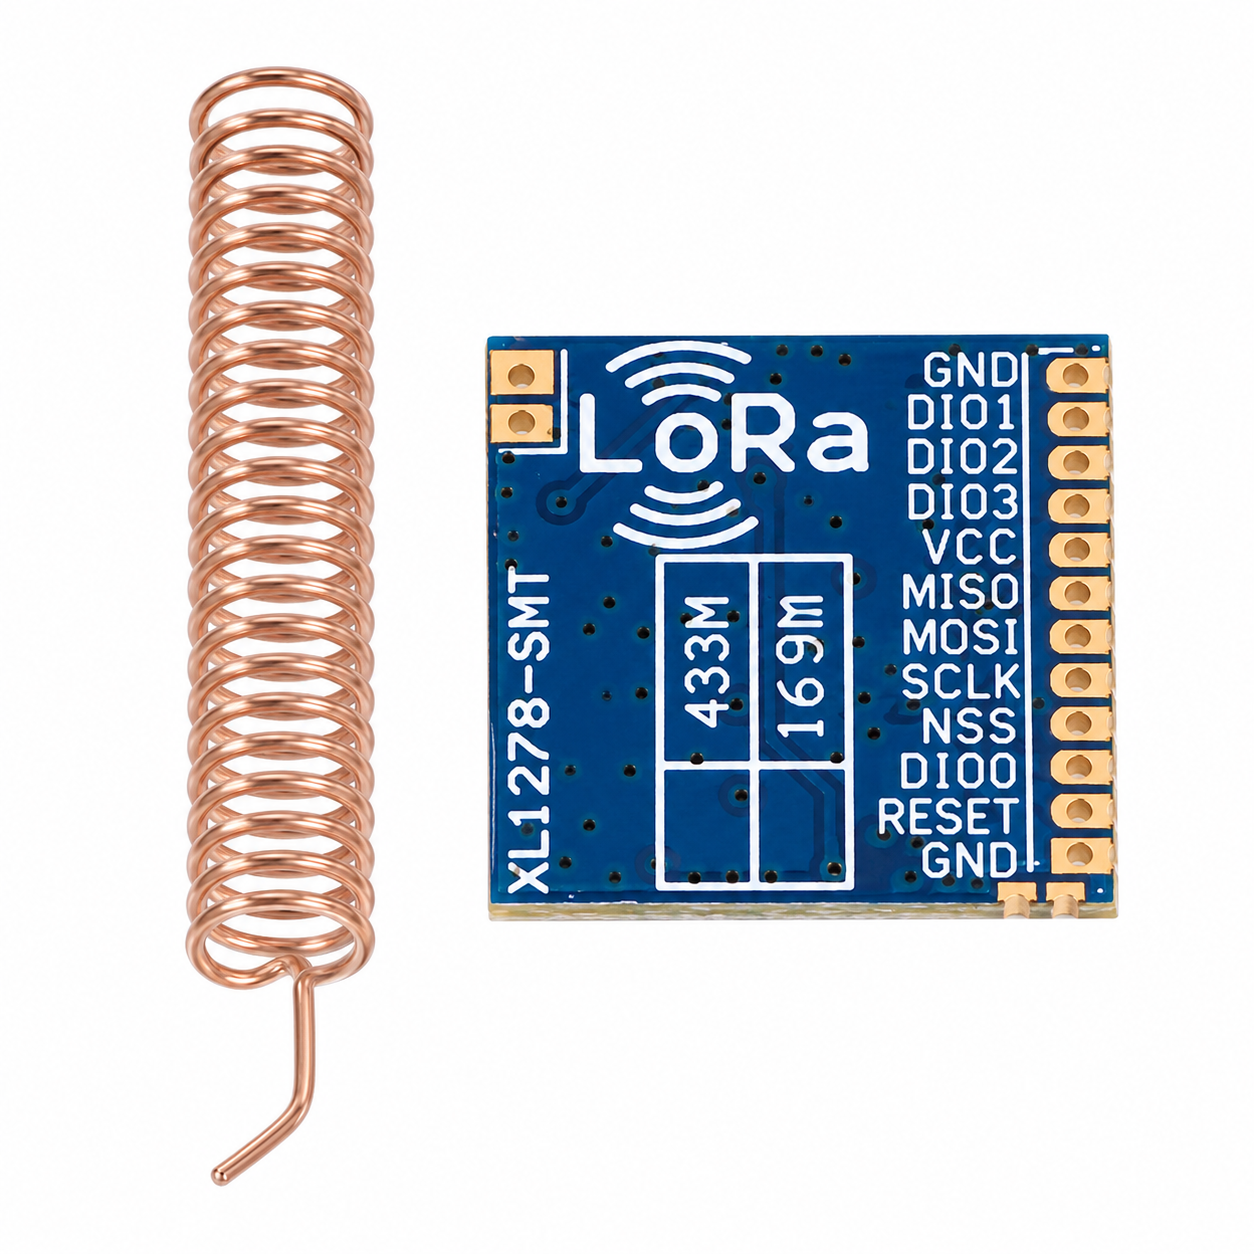
\includegraphics[width=0.45\textwidth]{figures/LoRa}
  \caption{LoRa transceiver module used for long-range wireless communication
           between distributed field nodes and the monitoring gateway.}
  \label{fig:lora-module-ch1}
\end{figure}

Table~\ref{tab:iot-communication-comparison} summarizes the main wireless
communication technologies considered for IoT agricultural field deployments,
comparing them on the criteria most relevant to outdoor, battery-powered, and
infrastructure-limited environments.

\begin{table}[H]
  \centering
  \caption{Comparison of wireless communication technologies for field IoT deployments.}
  \label{tab:iot-communication-comparison}
  \renewcommand{\arraystretch}{1.3}
  \begin{tabular}{|p{2.2cm}|p{2.2cm}|p{2.0cm}|p{2.4cm}|p{2.0cm}|p{2.2cm}|}
    \hline
    \textbf{Technology} & \textbf{Typical range} & \textbf{Power draw} &
    \textbf{Infrastructure} & \textbf{Cost} & \textbf{Field suitability} \\
    \hline
    Wi-Fi & 30–100\,m & Medium–High & Access points required & Low–Medium & Limited \\
    \hline
    Bluetooth/BLE & Up to 10\,m & Low & None & Low & Very limited \\
    \hline
    Zigbee & 100–300\,m per hop & Low & Coordinator node & Low & Moderate \\
    \hline
    GSM/4G & National coverage & High & Cellular network & High & High (where coverage exists) \\
    \hline
    LoRa & 1–15\,km & Very low & Gateway & Low & Very high \\
    \hline
  \end{tabular}
\end{table}

%---------------------------------------------------------------
\section{IoT Network Topologies}
\label{sec:topologies}
%---------------------------------------------------------------

Beyond the physical communication protocol, the arrangement of devices within a
network determines how data flows, where coordination occurs, and how the system
responds to individual node failures.

In a \textbf{point-to-point} topology, two devices communicate directly with each
other. This is the simplest arrangement and is adequate when a single sensor node
reports to a single receiver, but it does not scale to systems with multiple
sensing nodes.

A \textbf{star topology} places a central node, usually called a gateway or
coordinator, at the hub of the network. All sensing nodes communicate directly
with the gateway rather than with each other. The gateway aggregates incoming
measurements, manages acknowledgements, and handles the connection to any upstream
service. This topology is simple to implement, places minimal computational
demands on the sensing nodes, and provides a natural single point for data
collection and forwarding.

A \textbf{mesh topology} allows nodes to relay packets on behalf of each other,
enabling communication between nodes that are not within direct radio range of the
gateway. Mesh networks are more resilient to individual node failures but require
more complex routing protocols and firmware, which increases development effort
and power consumption on each node.

For distributed field monitoring with a small number of sensing nodes spread
across an agricultural site, the star topology is generally the most practical
choice. The gateway can be placed at a location with connectivity access, such as
a point where WiFi or mobile data is reachable for periodic uploads, while the
sensing nodes in the field require only enough radio range to reach it. This
matches the deployment scenario common in IoT agriculture
research~\cite{villa2020iot_arable_farming}.
% TODO: verify citation metadata for villa2020iot_arable_farming

The monitoring system described in this dissertation adopts a gateway-based star
topology using LoRa for field communication. The central gateway node coordinates
data reception from remote sensing nodes, manages local storage, and handles the
upload of collected measurements to the backend service. This organization aligns
with the topological principles described in this section and addresses the
practical constraints of field deployment outlined in
Section~\ref{sec:saharan-agriculture}.

%---------------------------------------------------------------
\section{Low-Power Operation in Field IoT Systems}
\label{sec:low-power}
%---------------------------------------------------------------

Battery-powered embedded nodes represent the practical reality of most distributed
agricultural deployments. Mains power is rarely accessible at precise sensor
placement locations within a field, and running power cables across dozens or
hundreds of metres introduces installation cost, maintenance burden, and the risk
of physical damage. The consequence is that the firmware design of a field node
must treat power consumption as a primary constraint rather than an afterthought.

The fundamental strategy in low-power embedded systems is to minimize the time
a device spends in high-power operating states. Modern microcontrollers support
deep sleep modes in which most internal peripherals are powered down and only
a timer or interrupt source remains active. During deep sleep, current draw can
fall several orders of magnitude below the active-mode consumption. A node that
wakes briefly to take a measurement, transmits a short packet, and returns to
sleep for several minutes or hours can operate for months on a modest battery.

\textbf{Duty cycling} is the general name for this wake-measure-sleep pattern.
Its effectiveness depends on keeping both the active period and the data volume
small. Sensor measurements are typically brief; the slower cost is often radio
communication, especially when retries or acknowledgement windows extend the
transmission period.

Peripheral power control is another dimension of low-power design. Sensors that
draw continuous current even when not being read can dominate the energy budget
of a sleeping device. Connecting such sensors through a relay or transistor switch
allows the microcontroller to power them only during measurement, eliminating
standby drain. Figure~\ref{fig:relay-power-control-ch1} shows the relay module
used in this project to control sensor power during low-power field operation.

\begin{figure}[H]
  \centering
  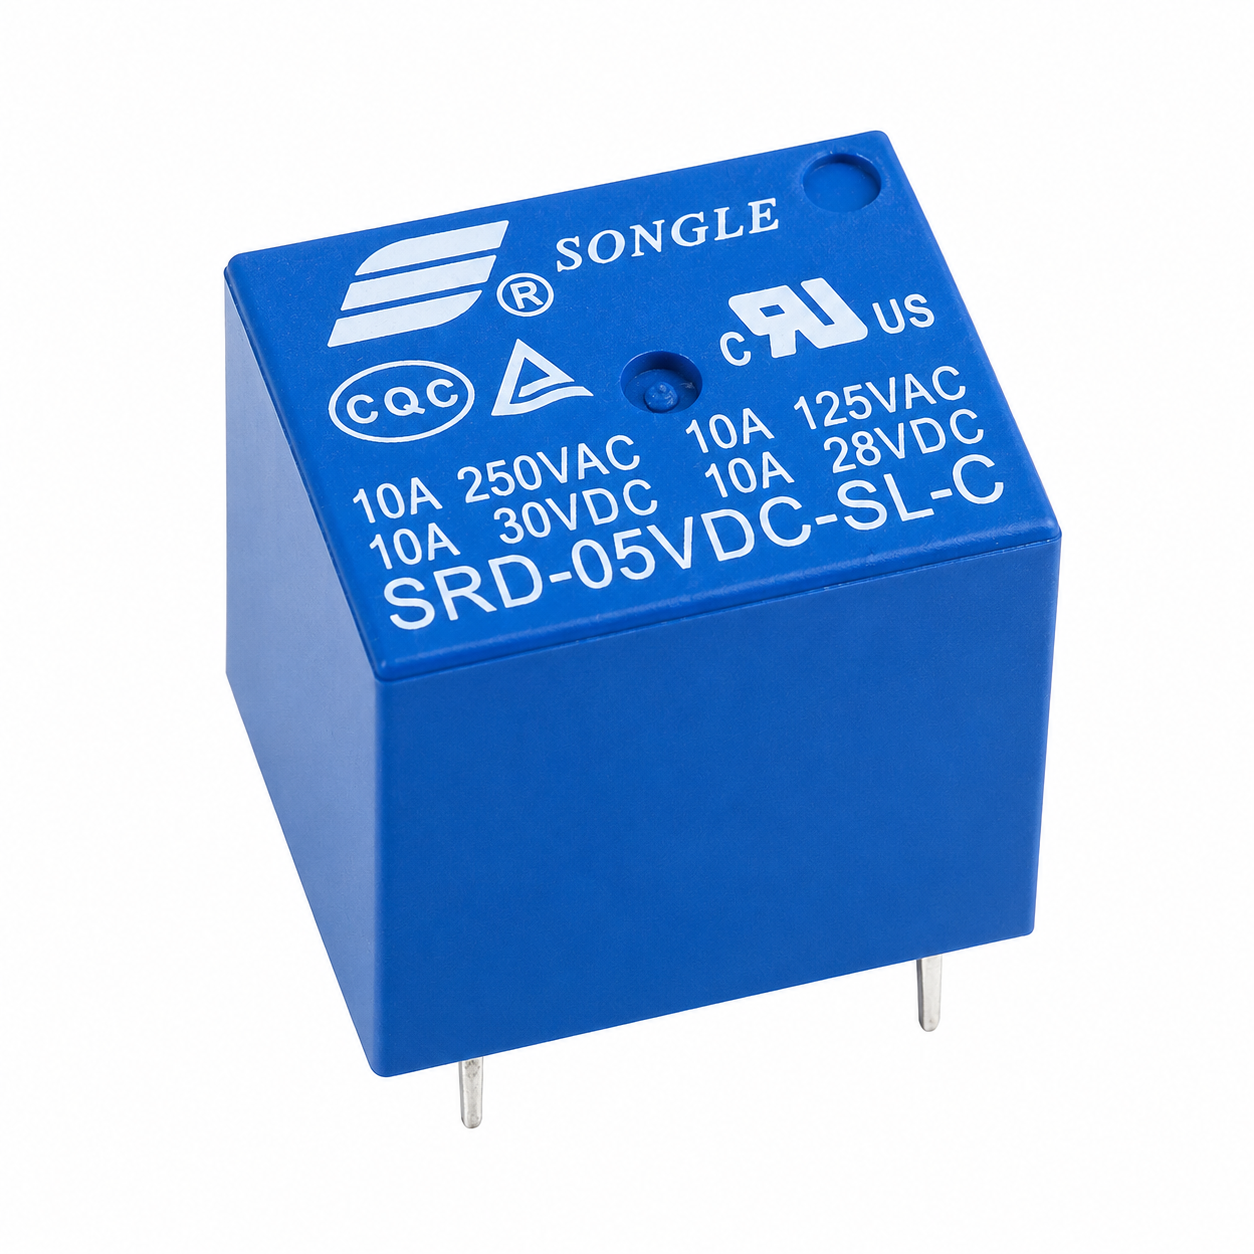
\includegraphics[width=0.35\textwidth]{figures/Relay}
  \caption{Relay module used to control sensor power, enabling measurement on
           demand while eliminating standby current consumption during sleep intervals.}
  \label{fig:relay-power-control-ch1}
\end{figure}

Environmental sensors present a specific case. The BME280 combined temperature,
humidity, and pressure sensor supports a \textit{forced mode} of operation in
which the sensor takes a single measurement triggered by the host microcontroller
and then returns to sleep automatically~\cite{bosch2024bme280_datasheet}. This
eliminates the need for the host to poll the sensor repeatedly or to manage its
active/sleep transitions manually, and it reduces both power consumption and the
risk of register-level programming errors. Figure~\ref{fig:bme280-sensor-ch1}
illustrates the BME280 module as used in the weather sensing node.

\begin{figure}[H]
  \centering
  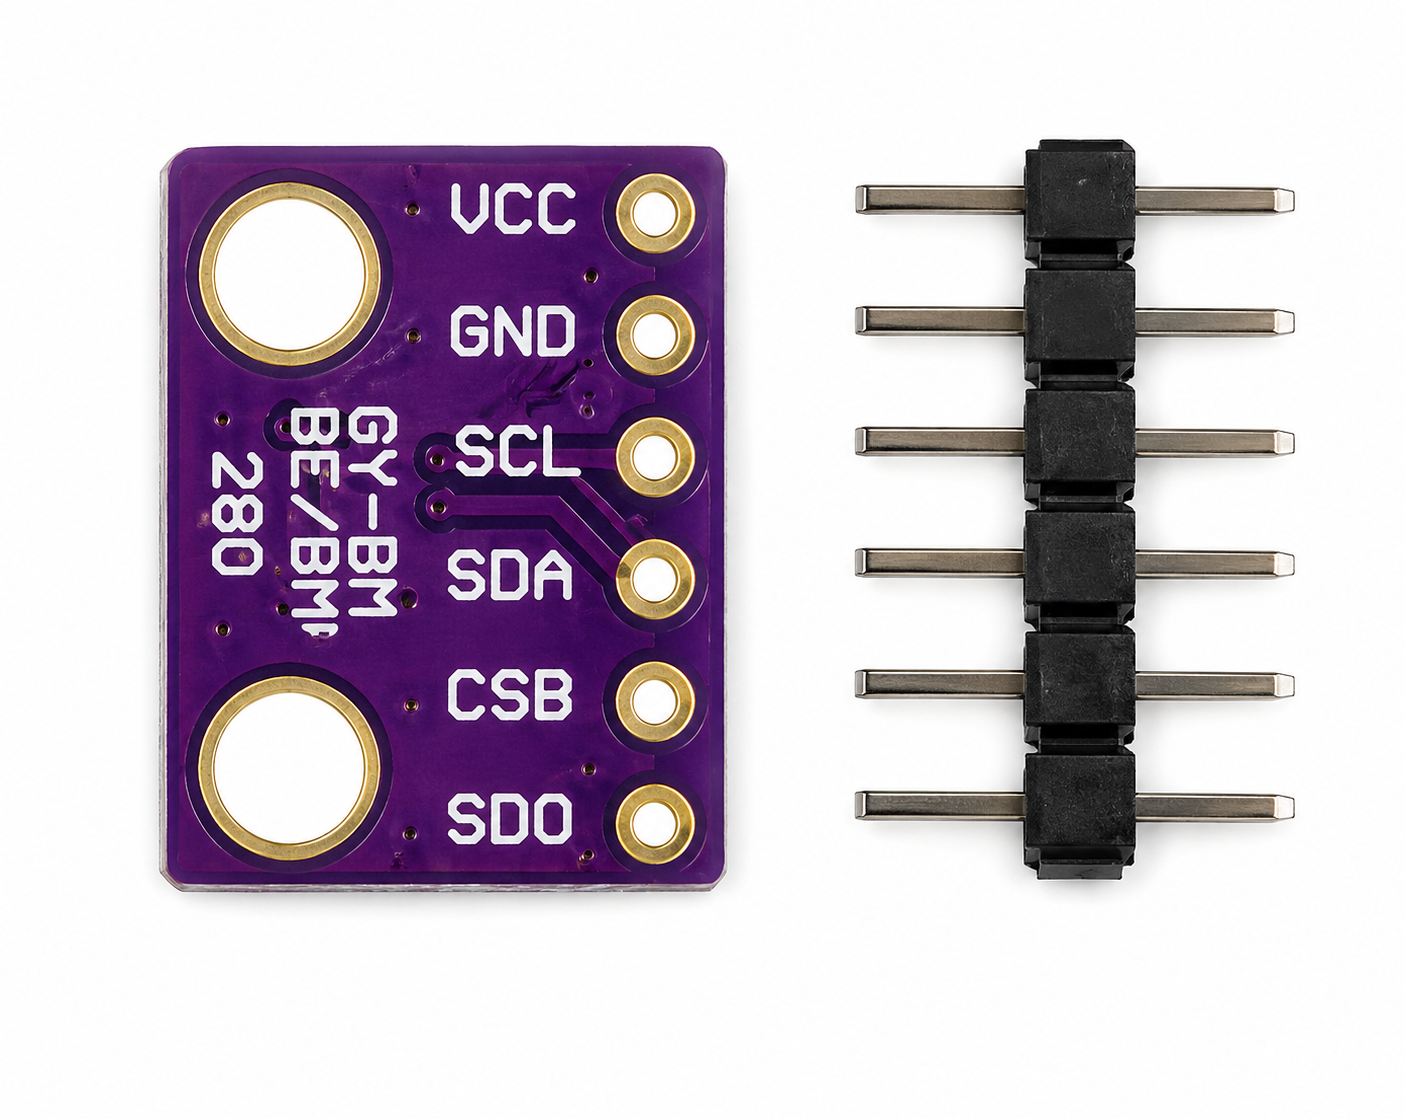
\includegraphics[width=0.40\textwidth]{figures/Bme280}
  \caption{BME280 environmental sensor module providing air temperature, relative
           humidity, and atmospheric pressure measurements in forced measurement mode.}
  \label{fig:bme280-sensor-ch1}
\end{figure}

The combination of deep sleep, duty cycling, relay-controlled sensor power, and
forced measurement mode allows a battery-powered field node to maintain a
meaningful measurement cycle over extended periods without requiring manual
intervention for battery replacement. The exact autonomy achievable depends on
battery capacity, cycle interval, and LoRa transmission parameters, and it
should be characterized experimentally for any specific deployment.

%---------------------------------------------------------------
\section{Reliability and Fault Recovery in IoT Systems}
\label{sec:reliability}
%---------------------------------------------------------------

The outdoor field environment is not a controlled laboratory. Radio signals are
subject to path loss, fading caused by vegetation or terrain, and interference
from other devices operating in the same frequency band. A packet that was
reliably received in bench testing may be lost when the gateway and node are
separated by a row of trees or when the antenna is positioned close to a metallic
surface. This variability is inherent to wireless communication and cannot be
eliminated entirely through hardware selection alone.

The practical consequence is that any field IoT system must be designed around
the assumption that some fraction of transmitted packets will not be received.
The question is how the system detects and responds to this situation.

An \textbf{acknowledgement} mechanism provides the most direct feedback. After
receiving a valid packet, the gateway transmits a short acknowledgement back to
the sender. If the sender does not receive the acknowledgement within a defined
window, it knows that the original packet may not have been received and can
attempt retransmission. This pattern reduces ambiguity and gives the sensing node
concrete information about whether its data reached the gateway.

Retransmission alone does not address a more subtle problem that can arise in
timed systems: \textbf{synchronization loss}. If a node operates on a fixed duty
cycle and misses several consecutive communication windows, the time offset
between the node's expected transmission window and the gateway's expected
reception window can grow. A node that wakes and transmits outside the gateway's
listening period will consistently fail to be received, even if the radio link is
technically functional. Recovery from this state requires a defined procedure
rather than simple retransmission.

Diagnostic event logging provides another layer of reliability management. When
a node misses its expected window, when the gateway fails to receive a packet it
expected, or when a recovery procedure is triggered, recording these events
creates an observable history of system behaviour. This history is valuable both
for real-time diagnostics and for post-hoc analysis of deployment conditions.
A reliability indicator derived from the ratio of received to expected packets is
one way to translate this event history into a metric that appears in dashboard
visualizations and analytics outputs.

%---------------------------------------------------------------
\section{Alfalfa Crop Background}
\label{sec:alfalfa-background}
%---------------------------------------------------------------

Alfalfa (\textit{Medicago sativa} L.) is a perennial leguminous forage crop grown
across a wide range of temperate, semi-arid, and arid environments. Its primary
agricultural role is as a high-quality animal feed: its leaf and stem biomass
provides a nutritionally dense fodder for cattle, sheep, and other livestock, and
its nitrogen-fixing root systems can contribute to long-term soil
fertility~\cite{fao_alflafa_crop_water}.

\subsection{Growth Cycle and Harvest Management}
\label{subsec:alfalfa-growth}

A distinguishing feature of alfalfa compared to annual crops is its perennial
regrowth habit. After an initial establishment period, the crop can be harvested
repeatedly throughout the growing season. Mueller and Teuber
\cite{mueller2007alfalfa_growth_development} describe typical cut cycles ranging
from four to twelve per year depending on climate, irrigation, and variety,
with each cycle proceeding through vegetative recovery, stem elongation, bud
initiation, and first-flower stages before harvest. The timing of each cut affects
both yield and forage quality: harvesting too early reduces biomass, while
delaying beyond the early flower stage lowers digestibility.

This repeated harvest cycle makes continuous monitoring practically beneficial.
Changes in soil moisture and temperature between cuts influence regrowth speed and
the timing of the next harvest decision. An operator who can observe the trend of
soil moisture following irrigation has better information for adjusting the next
irrigation event and for deciding when conditions are suitable for the next cut.

\subsection{Water and Irrigation Requirements}
\label{subsec:alfalfa-water}

Alfalfa is one of the more water-demanding forage crops, with seasonal
evapotranspiration requirements that vary by climate and
variety~\cite{irmak2007irrigation_alfalfa}. In arid and semi-arid environments,
where rainfall is insufficient to meet this demand, supplemental irrigation is
necessary throughout the growing season. Orloff et
al.~\cite{orloff2015drought_strategies_alfalfa} discuss the consequences of water
deficit at different growth stages and the options available to managers when
water supply is constrained, noting that strategic stress, which allows limited
moisture reduction between cuts, is more tolerable than severe deficit during
early regrowth.

For the monitoring system, these irrigation dynamics translate into a practical
need: soil moisture observations must be available before and after irrigation
events to support timing decisions and to document the effect of each irrigation
on the soil profile. Without this data, irrigation management relies on experience
and fixed schedules rather than observed soil conditions.

\subsection{Temperature Sensitivity and Heat Stress}
\label{subsec:alfalfa-heat}

Alfalfa growth is sensitive to thermal conditions. Wassie et
al.~\cite{wassie2019heat_stress_alfalfa} investigated the effects of elevated
temperatures on alfalfa physiology and observed reductions in photosynthetic rate,
leaf area, and shoot biomass under heat stress conditions. In Saharan regions
where summer temperatures regularly exceed 40°C, heat stress is a realistic
seasonal constraint rather than an exceptional event.

Air temperature monitoring therefore provides agronomically relevant context
beyond simple weather records. Observations of high air temperature during a
sensitive growth stage, cross-referenced with soil moisture and agronomic event
records, can help explain unexpected yield reductions or crop recovery patterns.

\subsection{Soil Conditions and Electrical Conductivity}
\label{subsec:alfalfa-soil}

Alfalfa establishes best in well-drained, slightly alkaline soils. It is
moderately tolerant of salinity but shows yield reductions as soil electrical
conductivity increases beyond threshold
levels~\cite{nrcs1999soil_electrical_conductivity}. In irrigated Saharan soils,
where repeated application of groundwater with variable mineral content can
gradually increase soil salinity, monitoring EC trends over time may reveal
deteriorating conditions before they become visible in plant symptoms.

Benabdelouahab et al.~\cite{benabdelouahab2019sensor_calibration_5te} examined the
laboratory calibration and field validation of a multi-parameter soil sensor
measuring moisture, temperature, and EC, and noted that raw in-situ EC values
depend on water content, temperature, and soil texture. This dependency means
that raw EC readings cannot be directly converted to saturated-paste ECe or to
official salinity classifications without appropriate calibration procedures
and reference soil samples. In the context of this project, soil EC is therefore
treated as a relative trend indicator rather than a diagnostic measurement.

\subsection{Summary of Monitoring Requirements}
\label{subsec:alfalfa-monitoring-summary}

Table~\ref{tab:alfalfa-monitoring-needs} summarizes the key agronomic variables
relevant to alfalfa cultivation and their monitoring significance in the context
of a field IoT platform.

\begin{table}[H]
  \centering
  \caption{Key monitoring variables for alfalfa cultivation and their agronomic
           significance in field IoT deployments.}
  \label{tab:alfalfa-monitoring-needs}
  \renewcommand{\arraystretch}{1.3}
  \begin{tabular}{|p{3.2cm}|p{5.0cm}|p{5.8cm}|}
    \hline
    \textbf{Variable} & \textbf{Agronomic relevance} & \textbf{Monitoring role} \\
    \hline
    Soil moisture & Irrigation scheduling; drought stress assessment;
                    cut-cycle timing & Track trends before and after irrigation;
                    compare pivot zones; support operator decisions \\
    \hline
    Soil temperature & Root zone activity; germination conditions;
                       freeze risk at depth & Contextual complement to air
                       temperature; interpretation of soil moisture trends \\
    \hline
    Soil electrical conductivity & Soil salinity trend; potential mineral
                                   accumulation from irrigation water &
                                   Relative trend indicator only; not a
                                   calibrated salinity diagnosis \\
    \hline
    Air temperature & Heat stress risk; growing-degree accumulation;
                      frost risk monitoring & Shared environmental context
                      for both pivot zones \\
    \hline
    Relative humidity & Vapour pressure deficit estimation; atmospheric
                        demand context & Weather context supporting
                        interpretation of soil moisture trends \\
    \hline
    Atmospheric pressure & General weather context; pressure trend
                           monitoring & Supporting environmental variable \\
    \hline
  \end{tabular}
\end{table}

%---------------------------------------------------------------
\section{Why Alfalfa Was Selected}
\label{sec:why-alfalfa}
%---------------------------------------------------------------

The selection of alfalfa as the target crop for this monitoring platform was not
arbitrary. It reflects a combination of regional economic relevance, practical
monitoring need, and a gap in the existing literature.

\subsection{Regional Importance and Demand}
\label{subsec:alfalfa-regional-importance}

Livestock production in Algeria and across the Maghreb region depends heavily on
cultivated fodder crops. Alfalfa is among the most productive and nutritionally
valuable options available, and its perennial nature means that a single
establishment investment supports multiple years of harvest. In the El Oued
region, alfalfa is cultivated in irrigated plots alongside other Saharan
agricultural products, and its contribution to local livestock feed supply gives
it direct economic significance.

The combination of high water demand, repeated cutting cycles, and sensitivity to
temperature and soil conditions makes alfalfa a crop where the benefits of
continuous automated monitoring are especially clear. A farmer managing several
pivot irrigation zones cannot practically visit each one after every cutting event
to assess soil recovery conditions. Remotely accessible, structured field data
fills this gap.

\subsection{The Crop-Specific Monitoring Gap}
\label{subsec:alfalfa-gap}

Reviewing the published literature on IoT-based agricultural monitoring reveals
that the majority of existing systems target general crops, greenhouse environments,
or irrigation automation without specifying the crop or focusing on its particular
monitoring requirements. Soil moisture sensing, LoRa communication, and web-based
dashboards appear frequently in the reviewed works, but alfalfa as a named target
crop is conspicuously absent from the systems encountered in this
review~\cite{ahmed2022lora_agriculture_chile,pereira2023esp32_drip_irrigation,saban2023smart_agricultural_lora_cloud}.

Within Algerian and Saharan agricultural research, some work has addressed desert
agriculture digitalization and smart agriculture applications at a general
level~\cite{iot_enhancements_algerian_desert_agriculture}.
% TODO: verify citation metadata for iot_enhancements_algerian_desert_agriculture
However, the combination of alfalfa crop focus, Saharan field conditions,
offline-first data collection, and deterministic analytics has not been
explicitly addressed in the works identified during the literature review
process. This gap is not stated as a universal absolute; it reflects the scope
of the works reviewed. It is nonetheless a meaningful observation that justifies
the specific framing of this project.

\subsection{Multiple Cutting Cycles as a Monitoring Driver}
\label{subsec:alfalfa-cycles}

The repeated-harvest nature of alfalfa distinguishes it from annual crops in a
way that is particularly relevant to monitoring system design. Each cutting event
resets the soil moisture dynamic: root zone activity temporarily declines, water
uptake slows, and the soil dries differently than during active vegetative growth.
Post-cut irrigation and its effect on soil moisture recovery are therefore
observable events that a time-series monitoring system can capture and document.

For a monitoring platform that separates manual agronomic event records from
automatic sensor measurements, this cycle provides a natural opportunity for
contextual alignment. Recorded irrigation events can be compared with observed
soil moisture trends, and the time between cutting and regrowth can be tracked
against environmental conditions. These are the kinds of relationships that
structured agricultural data makes possible — not as automatic agronomic
decisions, but as information that supports better-informed human decisions.

%---------------------------------------------------------------
\section{Chapter Summary}
\label{sec:ch1-summary}
%---------------------------------------------------------------

This chapter established the theoretical and contextual foundations on which the
proposed monitoring platform is built. The starting point was the Saharan
agricultural environment: harsh temperatures, scarce rainfall, unstable power
supply, and remote field locations that make continuous manual monitoring both
impractical and insufficient.

The discussion of agricultural data collection highlighted that sensor readings
alone are not enough. Traceability, timestamp integrity, and domain separation
between measurements, events, transfer records, and agronomic context are
necessary conditions for data that can be reliably analysed and interpreted.
The smart agriculture and IoT background showed that effective monitoring systems
are organized in layers, with clear responsibilities at each stage of the data
lifecycle, and that the distinction between monitoring and autonomous control has
practical consequences for what a system can and cannot claim.

The communication technology comparison demonstrated why LoRa is well-suited to
distributed field monitoring over distances typical of agricultural sites, given
its combination of range, low power consumption, and freedom from cellular
infrastructure. The network topology discussion reinforced the suitability of
a gateway-based star arrangement for coordinating a small number of sensing nodes
with a central collection point.

Low-power operation and fault recovery were presented as two constraints that
every field IoT design must address explicitly. Deep sleep, duty cycling,
peripheral power control, acknowledgement-based communication, and diagnostic
event logging are not optional refinements; they are design requirements for
systems intended to operate reliably in environments where power is limited and
radio communication is imperfect.

Finally, the alfalfa agronomic background connected the technical infrastructure
to its intended purpose. Soil moisture, soil temperature, soil electrical
conductivity, air temperature, humidity, and atmospheric pressure are the
variables that matter for the crop. The repeated harvest cycle creates natural
opportunities for structured observation, and the absence of dedicated alfalfa
monitoring studies in local Saharan contexts provides a specific motivation for
this work.

The following chapter examines how related works have approached agricultural IoT
monitoring, identifies what they contribute and where their limitations lie, and
uses this comparative analysis to position the proposed system within the broader
field of smart agriculture research.

\clearpage

%===============================================================
% Chapter 2 — Related Works and Comparative Analysis
% Part A: Sections 2.1–2.10
% Thesis: A Smart Farm IoT Monitoring and Deterministic Agronomic
%         Analytics Platform for Alfalfa Cultivation
% Authors: Abderrahmane Henna · Nacer Eddine Aouissi
% Supervisor: Mohib Eddine KHEBBACHE
% University of El Oued – Echahid Hamma Lakhdar, 2025/2026
%===============================================================

\chapter{Related Works and Comparative Analysis}
\label{chap:related-works}

%---------------------------------------------------------------
\section{Chapter Introduction}
\label{sec:ch2-intro}
%---------------------------------------------------------------

The previous chapter established the theoretical and contextual foundations of
this work: the constraints of Saharan field environments, the data collection
principles that govern a reliable monitoring system, the communication and
topology choices relevant to distributed IoT deployments, and the agronomic
requirements of alfalfa cultivation. Those foundations were drawn from general
literature and technical standards. This chapter moves from general principles to
the specific: it examines how previous research has addressed agricultural IoT
monitoring, what these works have achieved, and where meaningful gaps remain.

The analysis is organized thematically rather than as a sequential list of papers.
Seven dimensions guide the comparison: system architecture and monitoring scope,
wireless communication strategies, soil and environmental data collection,
energy management and field reliability, offline storage and upload handling,
timestamp semantics and data integrity, and dashboard plus analytics design.
A dedicated section then surveys the crop contexts addressed by the reviewed
works, leading to an explicit identification of the alfalfa monitoring gap that
motivates this project.

The chapter draws primarily on three peer-reviewed works that are close enough
to this project to support meaningful comparison: Ahmed et al.
(2022)~\cite{ahmed2022lora_agriculture_chile}, Pereira et al.
(2023)~\cite{pereira2023esp32_drip_irrigation}, and Saban et al.
(2023)~\cite{saban2023smart_agricultural_lora_cloud}. Supporting references
from survey works~\cite{ayaz2019iot_smart_agriculture_survey,farooq2019iot_smart_agriculture_review}
and data quality literature~\cite{teh2020sensor_data_quality,dandrifosse2024weather_qc_agriculture}
provide broader context. Where additional works are referenced and their
bibliographic metadata requires verification, this is noted explicitly.

%---------------------------------------------------------------
\section{IoT-Based Agricultural Monitoring Systems}
\label{sec:iot-monitoring-systems}
%---------------------------------------------------------------

Field-oriented IoT monitoring systems have converged on a recognizable pattern
over the past decade: embedded sensing nodes collect environmental or soil
measurements, a wireless link carries those measurements to a receiver or
gateway, and a web-based interface makes the data accessible to users.
Surveys of the field confirm that this three-layer structure is the dominant
approach~\cite{ayaz2019iot_smart_agriculture_survey,farooq2019iot_smart_agriculture_review}.
Within this shared architecture, individual systems differ significantly in
the variables they monitor, the embedded hardware they use, and the
infrastructure they assume.

ESP32-based nodes appear frequently across recent implementations. Pereira et
al.~\cite{pereira2023esp32_drip_irrigation} present an IoT system built around
the ESP32 microcontroller for smart drip irrigation, integrating soil and
environmental sensing with a cloud-connected dashboard for visualization and
control. The system's primary objective is irrigation automation: the ESP32
measures soil conditions, evaluates them against thresholds, and triggers the
irrigation mechanism accordingly. This is a coherent design for its intended
purpose, and the use of ESP32 as the embedded platform reflects its practical
balance of processing capability, wireless connectivity, and cost. The
limitation relative to this project's goals is one of scope rather than
technical error: the system is designed for irrigation control of a general
crop, not for multi-node field monitoring with multi-domain data governance,
manual agronomic event recording, and an explicit analytical layer targeted at
a specific crop.

Ahmed et al.~\cite{ahmed2022lora_agriculture_chile} approach the monitoring
problem at a different scale. Their LoRa-based platform is deployed across a
large commercial farm in Chile and focuses on remote sensing, LoRa network
behavior, and multi-point data collection. The platform demonstrates that LoRa
communication can sustain reliable data delivery across agricultural field
distances, and the multi-layer system architecture covers sensor nodes, a
gateway, and a server-side monitoring interface. What the work foregrounds is
the feasibility of LoRa as a field communication technology. What it does not
foreground is the data governance layer: the distinction between measurement
time and upload time, the handling of the data record during connectivity
outages, or the reliability of individual readings relative to a quality
control standard.

Saban et al.~\cite{saban2023smart_agricultural_lora_cloud} combine PLC-based
field control with a LoRa/LoRaWAN communication infrastructure and a
cloud-hosted web application for monitoring and device management. The system
extends the monitoring concept toward active agricultural management, and the
cloud web interface provides a relatively complete view of connected devices
and their states. The architecture, however, is fundamentally cloud-first:
field data is expected to reach the server promptly, and the system's
monitoring and control functions operate on this assumption. The treatment of
offline periods, local data persistence, or upload audit trails is not the
central contribution of the work.

Across these systems, the sensing and visualization layers are the primary
technical contributions. The data infrastructure connecting them --- how
measurements are timestamped at the moment of collection, how the local record
is preserved when the network is unavailable, and how uploaded data is
validated against expected structure and timing --- receives comparatively
limited attention. This is not a deficiency in individual papers; it reflects
where the research effort has been directed. It does, however, identify a
space in which the system proposed in this dissertation makes a specific
contribution.

%---------------------------------------------------------------
\section{Wireless Communication in Agricultural IoT}
\label{sec:wireless-communication}
%---------------------------------------------------------------

The appropriateness of LoRa as a field communication technology was established
in Chapter~\ref{chap:background} through a comparison of wireless protocol
characteristics. The reviewed works confirm this choice empirically: both Ahmed
et al.~\cite{ahmed2022lora_agriculture_chile} and Saban et
al.~\cite{saban2023smart_agricultural_lora_cloud} deploy LoRa in agricultural
environments and demonstrate that the technology can sustain data delivery
across field-scale distances with acceptable power budgets.

The practical question that emerges from these works is not whether LoRa can
carry data across a field, but what guarantees accompany delivery. Ahmed et
al.\ demonstrate multi-point remote monitoring with LoRa and discuss network
behavior at the farm scale, including link quality observations. Saban et al.\
use LoRaWAN infrastructure, which adds a network server layer that handles
some aspects of device management and downlink communication. In both cases,
the communication architecture is the subject of design attention. What is less
discussed is the upstream consequence of communication uncertainty: when a
field node fails to transmit successfully, how does the system detect this, log
it, and recover?

Communication feasibility and communication reliability are related but not
identical. A LoRa link that works ninety percent of the time is highly
functional for many monitoring purposes, but the ten percent of missed packets
creates gaps in the server-side record that may not be distinguishable from
periods of genuine field inactivity. If the only signal of a problem is a gap
in the database, an operator looking at a dashboard chart cannot easily
determine whether the crop conditions were stable and unreported, or whether
the node failed and the sensor data was never acquired.

Addressing this requires more than the communication layer alone. An
acknowledgement mechanism at the application level, a diagnostic event log
that records missed transmissions and recovery attempts, and a recovery
procedure for nodes that have drifted out of synchronization with the gateway's
receive window all contribute to turning communication feasibility into
operational reliability. The works reviewed here lay a strong foundation for
the communication design; the proposed system builds on that foundation by
adding the reliability and logging infrastructure on top of the communication
layer.

Regarding outdoor protocol selection more broadly, work on the effects of
communication protocols in precision agriculture outdoor
environments~\cite{iot_protocols_precision_agriculture_outdoor} offers
additional empirical context for understanding how environmental conditions
affect protocol
performance.
% TODO: verify bibliographic metadata for iot_protocols_precision_agriculture_outdoor before final submission

%---------------------------------------------------------------
\section{Soil and Environmental Data Collection Systems}
\label{sec:soil-environmental}
%---------------------------------------------------------------

Soil moisture is the most frequently monitored variable in agricultural IoT
systems, and with good reason: it is the primary determinant of irrigation
timing, a sensitive indicator of crop water status, and a variable that changes
on timescales short enough to make periodic automated measurement practically
useful~\cite{ayaz2019iot_smart_agriculture_survey}. Environmental variables
--- air temperature, humidity, and atmospheric pressure --- appear alongside
soil measurements in many systems as contextual information that helps
interpret the soil data.

The design of the data collection pipeline receives varying degrees of
attention across the reviewed works. Most systems describe the sensing hardware
and the dashboard interface in detail, with the data pathway between them
treated as a solved problem of wireless transmission and database storage.
Wireless sensor network deployments focused specifically on soil moisture
monitoring~\cite{lloret2021soil_moisture_wsn} address aspects of sensor
placement, network topology, and data reliability in that
context.
% TODO: verify bibliographic metadata for lloret2021soil_moisture_wsn before final submission
Studies on practical, low-cost IoT solutions for agricultural data
monitoring~\cite{cheap_practical_iot_agri_monitoring} address deployment
feasibility in resource-constrained
settings.
% TODO: verify bibliographic metadata for cheap_practical_iot_agri_monitoring before final submission

What these systems share is a primary focus on the measurement itself: which
sensor to use, where to place it, and how to transmit its reading. Less
consistently addressed is the organization of the collected data once it
arrives at the server: whether soil and weather data are stored in separate
structured domains, whether individual readings carry quality indicators, and
whether the collection pipeline distinguishes between data that represents a
valid measurement and data that represents a recovered or estimated value.

A related challenge is the multi-source nature of agricultural monitoring
data. Even a relatively simple field setup produces at least two categories of
information: automatic sensor readings and human-entered agronomic records such
as irrigation events and cutting dates. Keeping these categories separate, with
appropriate timestamps for each, allows later analysis to use both without
conflating machine-generated and human-entered information. Teh et
al.~\cite{teh2020sensor_data_quality} identify data completeness and
consistency as critical quality dimensions that must be managed across the full
data lifecycle, not only at the sensor interface. In most reviewed systems,
this lifecycle management is implicit rather than a named design objective.

Pereira et al.~\cite{pereira2023esp32_drip_irrigation} combine soil sensing
with irrigation control in a system that uses sensor measurements to drive
direct actuation. The monitoring and control functions are tightly coupled,
which is appropriate for an irrigation automation system. For a system focused
on monitoring and decision support for a specific crop, however, the separation
between what the system measures and what the operator decides remains
important. Coupling measurement to automatic action blurs this distinction.

%---------------------------------------------------------------
\section{Energy Management and Field Reliability}
\label{sec:energy-reliability}
%---------------------------------------------------------------

Battery-powered field nodes are a practical reality in distributed agricultural
monitoring, and managing power consumption is a standard design challenge. The
reviewed works acknowledge this constraint at different levels of depth.

At the hardware selection level, the choice of microcontroller, radio module,
and sensor type all affect the power budget. ESP32-based systems, as used by
Pereira et al.~\cite{pereira2023esp32_drip_irrigation}, benefit from the
availability of deep sleep modes that reduce current draw significantly during
idle periods. LoRa radios, as used by both Ahmed et
al.~\cite{ahmed2022lora_agriculture_chile} and Saban et
al.~\cite{saban2023smart_agricultural_lora_cloud}, are selected partly for
their low transmission power relative to cellular alternatives.

Energy-aware firmware design is less consistently detailed in the reviewed
works. Duty cycling --- the pattern of wake, measure, transmit, sleep --- is
implied by most field node designs but is not always described in terms of its
effect on measurement continuity or its interaction with the communication
window. The relationship between the node's sleep interval, the gateway's
receive window, and the risk of timing drift between the two is a specific
firmware engineering concern that is rarely foregrounded as a primary design
topic.

A related aspect of field reliability is the system's ability to recover from
communication failures without manual intervention. Pereira et
al.~\cite{pereira2023esp32_drip_irrigation} address retry mechanisms at the
sensor-actuator level. Ahmed et al.~\cite{ahmed2022lora_agriculture_chile}
discuss network performance and link quality. Neither work centers on the
problem of a node that has lost synchronization with the gateway's receive
window and must execute a defined recovery procedure before normal operation
can resume. This distinction between temporary packet loss and timing
desynchronization is subtle but consequential in systems that depend on
coordinated duty cycles.

A broader review of data collection architectures in IoT
networks~\cite{abbaari2024data_collection_iot_networks} discusses reliability
challenges at the network and protocol level, confirming that reliability is a
recognized concern in the IoT literature, even when specific firmware-level
recovery procedures are not detailed in individual
systems.
% TODO: verify bibliographic metadata for abbaari2024data_collection_iot_networks before final submission
A review of smart sensors and their deployment challenges in agricultural
contexts~\cite{rajak2023iot_smart_sensors_agriculture} similarly identifies
reliability and energy as ongoing concerns without providing field-level
recovery
procedures.
% TODO: verify bibliographic metadata for rajak2023iot_smart_sensors_agriculture before final submission

Diagnostic event logging complements energy and reliability design. When a
node misses its expected window, when a recovery attempt is made, or when a
communication failure is resolved, recording these events creates an auditable
history that can inform both real-time dashboard diagnostics and retrospective
reliability analysis. In most reviewed systems, such logging is either absent
or described as a debugging tool rather than a primary feature of the data
model.

%---------------------------------------------------------------
\section{Offline Storage and Upload Strategies}
\label{sec:offline-storage}
%---------------------------------------------------------------

Many agricultural IoT systems are designed with the implicit assumption that
a network connection is available for data forwarding on a timescale
comparable to the measurement interval. Cloud-first architectures, in which
sensor readings are transmitted to a remote server shortly after collection,
are practical when connectivity is reliable. In Saharan and remote field
environments of the kind described in Section~\ref{sec:saharan-agriculture},
this assumption is not always valid.

Ahmed et al.~\cite{ahmed2022lora_agriculture_chile} deploy their platform
across a large commercial farm with LoRa gateways and server-side
infrastructure in place. The architecture assumes that the gateway has
connectivity to forward data to the cloud server. Saban et
al.~\cite{saban2023smart_agricultural_lora_cloud} use a LoRaWAN network server
and a cloud-hosted web application, again assuming that the gateway is
continuously connected to the upstream service. Pereira et
al.~\cite{pereira2023esp32_drip_irrigation} connect the ESP32 to a cloud
service for dashboard access. In each case, the data path leads promptly from
field to cloud.

The consequence of this design is that the server-side record is only as
complete as the connectivity allows. A period of network unavailability
produces a gap in the database that may be indistinguishable from a period
where no field data existed. An offline-first design inverts this priority:
measurements are stored locally before any upload attempt, and the upload
is an explicit, operator-controlled action rather than an automatic background
process. Under this model, the local record is always complete; the server-side
record is a subset of the local record determined by when uploads occurred.

The distinction between when data is uploaded and when it was measured is
therefore not merely a technical detail. It is the design choice that
determines whether a gap in the server database represents an absence of
field data or a delay in its transfer. Treated differently in analytics, these
two interpretations lead to different conclusions about field conditions and
system reliability.

%---------------------------------------------------------------
\section{Time Synchronization and Data Integrity}
\label{sec:time-sync}
%---------------------------------------------------------------

Every data record in a time-series monitoring system carries a timestamp, and
the meaning of that timestamp determines what the record represents. Whether
the timestamp records the moment of measurement, the moment of local storage,
the moment of transmission, or the moment of server-side ingestion is not
always explicitly defined in the reviewed works. In systems with low latency
between measurement and cloud arrival, the difference is small enough to be
negligible. In systems where data can rest on local storage for hours or days
before upload, the distinction becomes analytically significant.

Dandrifosse et al.~\cite{dandrifosse2024weather_qc_agriculture} illustrate
this in the context of agricultural weather data: quality control algorithms
that rely on observation timestamps produce incorrect results when those
timestamps reflect processing time rather than measurement time. The point
applies equally to soil sensor data. A soil moisture reading labelled with the
upload timestamp rather than the measurement timestamp will appear on a chart
at the wrong point in time, potentially misrepresenting the relationship
between soil conditions and agronomic events such as irrigation.

The reviewed works address timestamp handling with varying degrees of
explicitness. Ahmed et al.~\cite{ahmed2022lora_agriculture_chile} focus on the
communication layer and the monitoring platform; the question of which
timestamp propagates through the system and serves as the chart time axis is
not a primary discussion topic. Saban et
al.~\cite{saban2023smart_agricultural_lora_cloud} focus on control and
monitoring through the cloud interface; timestamp semantics at the field node
level are similarly not foregrounded. Pereira et
al.~\cite{pereira2023esp32_drip_irrigation} focus on the irrigation control
logic; the time axis of the sensor readings is not the central concern.

In a system where offline storage and batch upload are by design, timestamp
integrity requires an active approach. The field node must assign measurement
timestamps at the moment of sensing, using a time source that does not depend
on network availability. A dedicated real-time clock module, synchronized
periodically to a reference source and used consistently as the timestamp for
every measurement, provides this guarantee. The clock synchronization
procedure itself must be explicit and auditable, so that an operator can
confirm when the clock was last synchronized and what the expected drift is
between synchronization events.

This approach --- authoritative field-assigned measurement timestamps,
preserved through local storage and batch upload, and used as the sole time
axis for analytics --- is the design choice this dissertation makes and that
the reviewed works do not explicitly address.

%---------------------------------------------------------------
\section{Dashboards, Analytics, and AI Interpretation}
\label{sec:dashboards-analytics-ai}
%---------------------------------------------------------------

Web-based dashboard interfaces appear in all three primary reference systems
as the final layer of user interaction. Ahmed et
al.~\cite{ahmed2022lora_agriculture_chile} provide a monitoring platform with
sensor data visualization. Saban et
al.~\cite{saban2023smart_agricultural_lora_cloud} include a cloud-hosted web
interface for monitoring and device control. Pereira et
al.~\cite{pereira2023esp32_drip_irrigation} implement a dashboard for
visualizing sensor readings and managing irrigation parameters.

These interfaces fulfill the primary function of a monitoring dashboard:
making field data visible to the operator through charts, status indicators,
and historical views. Where they differ from the dashboard proposed in this
work is in the depth of the analytics layer between raw data and displayed
information. A typical monitoring dashboard passes measurements from the
database to the chart directly, possibly with basic filtering and
aggregation. A dashboard backed by a deterministic analytics layer first
applies quality control rules to identify anomalous or unreliable readings,
computes reliability indicators based on the completeness and consistency of
the data record, and makes the results of both the raw and the processed data
visible to the user.

The distinction between raw measurement display and processed data
transparency matters for two reasons. First, an operator looking at a soil
moisture chart cannot easily distinguish a genuine measurement from one that
is the result of a sensor glitch, a duplicate upload, or a timestamp anomaly
--- unless the dashboard makes this distinction explicit. Second, when
analytics outputs are derived from cleaned and quality-controlled data, the
chain from raw reading to displayed result should be traceable, so that a
discrepancy between a sensor reading and an analytics indicator can be
investigated rather than simply accepted.

Regarding artificial intelligence: some recent agricultural systems have
explored machine learning components for prediction, anomaly detection, or
crop state estimation. This is a legitimate research direction, but it
introduces an important boundary question. When AI generates a result ---
whether a prediction, a recommendation, or a summary --- the basis for that
result should be distinguishable from the basis for deterministic metrics
computed by rule-based or statistical methods. Treating AI output as
equivalent to a sensor reading or a reliability score conflates two
fundamentally different types of information.

The approach adopted in this project positions the AI component strictly as
an interpretation layer. Deterministic analytics --- quality control,
reliability scoring, and trend metrics --- are computed independently of any
AI model. The AI component receives the outputs of these deterministic steps
and provides a narrative explanation. It does not compute primary metrics,
fill missing measurements, or override reliability assessments. This boundary
is intentional and is reflected throughout the system architecture.

%---------------------------------------------------------------
\section{Previous Crop Targets in Existing Works}
\label{sec:crop-targets}
%---------------------------------------------------------------

Reviewing the agricultural context of the selected related works reveals a
consistent pattern. Most systems target general irrigation applications,
unspecified crop environments, or broad smart agriculture goals. None of the
primary works reviewed for this chapter targets alfalfa as the principal
monitored crop. Table~\ref{tab:related-work-crop-focus} summarizes the crop
focus and main technical contribution of each reviewed work.

\begin{table}[H]
  \centering
  \caption{Crop context and primary technical focus of selected related works
           reviewed in this chapter.}
  \label{tab:related-work-crop-focus}
  \renewcommand{\arraystretch}{1.3}
  \begin{tabular}{|p{3.8cm}|p{2.4cm}|p{3.6cm}|p{1.4cm}|p{2.0cm}|}
    \hline
    \textbf{Work} & \textbf{Crop / context} & \textbf{Main technical focus} &
    \textbf{Alfalfa target?} & \textbf{Thesis relevance} \\
    \hline
    Ahmed et al.~\cite{ahmed2022lora_agriculture_chile} (2022) &
    Large-scale farms, Chile &
    LoRa IoT monitoring platform &
    No & LoRa architecture comparison \\
    \hline
    Pereira et al.~\cite{pereira2023esp32_drip_irrigation} (2023) &
    General irrigation &
    ESP32 smart drip irrigation &
    No & Embedded sensing comparison \\
    \hline
    Saban et al.~\cite{saban2023smart_agricultural_lora_cloud} (2023) &
    General smart agriculture &
    PLC + LoRa/LoRaWAN + cloud web app &
    No & Cloud dashboard comparison \\
    \hline
    Ayaz et al.~\cite{ayaz2019iot_smart_agriculture_survey} (2019) &
    Multiple crops (survey) &
    IoT smart agriculture survey &
    No & Smart agriculture background \\
    \hline
    Farooq et al.~\cite{farooq2019iot_smart_agriculture_review} (2019) &
    Multiple crops (review) &
    IoT smart farming review &
    No & Smart farming context \\
    \hline
    Rajak et al.~\cite{rajak2023iot_smart_sensors_agriculture} &
    % TODO: verify bibliographic metadata for rajak2023iot_smart_sensors_agriculture before final submission
    Generic IoT agriculture &
    Smart sensors review &
    No & Sensor deployment context \\
    \hline
    Villa-Henriksen et al.~\cite{villa2020iot_arable_farming} &
    % TODO: verify bibliographic metadata for villa2020iot_arable_farming before final submission
    Arable farming (general) &
    IoT challenges and opportunities &
    No & Broad IoT farming review \\
    \hline
    Abbaari et al.~\cite{abbaari2024data_collection_iot_networks} &
    % TODO: verify bibliographic metadata for abbaari2024data_collection_iot_networks before final submission
    IoT networks (general) &
    Data collection architecture &
    No & Data collection theory \\
    \hline
    Cheap practical IoT~\cite{cheap_practical_iot_agri_monitoring} &
    % TODO: verify bibliographic metadata for cheap_practical_iot_agri_monitoring before final submission
    Generic agricultural &
    Low-cost IoT monitoring &
    No & Practical IoT context \\
    \hline
    Lloret et al.~\cite{lloret2021soil_moisture_wsn} &
    % TODO: verify bibliographic metadata for lloret2021soil_moisture_wsn before final submission
    Soil moisture monitoring &
    Wireless soil moisture WSN &
    No & Soil sensing comparison \\
    \hline
  \end{tabular}
\end{table}

The observation that none of the reviewed works targets alfalfa is not in
itself a gap; most monitoring systems are intentionally general and their
value does not depend on crop specificity. The gap emerges when considered
alongside the monitoring requirements established in
Section~\ref{subsec:alfalfa-monitoring-summary}: the repeated cutting cycle,
the soil moisture dynamics between cuts, the need for contextual alignment
between sensor trends and agronomic events, and the specific field conditions
of Saharan oasis cultivation.

%---------------------------------------------------------------
\section{The Alfalfa Monitoring Gap}
\label{sec:alfalfa-gap}
%---------------------------------------------------------------

The practical significance of a monitoring system depends partly on whether
its design reflects the specific requirements of the crop it serves. A system
built for general irrigation scheduling imposes no particular structure on how
field data should be organized around cutting events, how soil moisture trends
before and after an irrigation event should be captured and compared across
different irrigated zones, or how the monitoring timeline aligns with the
biological cycle of the crop. For alfalfa, these are not abstract concerns ---
they are the questions that a monitoring platform must help an operator answer.

Alfalfa's repeated harvest pattern means that the monitoring cycle is not
seasonal in the conventional sense. Multiple cut events occur within a single
growing season, each resetting the soil moisture dynamic and creating a new
period of vegetative regrowth that must be monitored for irrigation timing.
Chapter~\ref{chap:background} established that alfalfa is sensitive to soil
moisture deficit, heat stress, and soil electrical conductivity changes, and
that each of these variables can be monitored with appropriate field sensors.
What the background chapter could not establish from the literature is whether
any existing IoT monitoring system has been designed around this crop in a
Saharan or Algerian context.

Within the works reviewed for this thesis, no selected related work
explicitly targets alfalfa as the monitored crop. The works reviewed focus on
general irrigation systems, unspecified commercial crops, or broad smart
agriculture goals in geographic and climatic settings different from the
Saharan oasis environment. Some work on IoT enhancements specific to Algerian
desert agriculture~\cite{iot_enhancements_algerian_desert_agriculture} touches
on the regional context,
% TODO: verify bibliographic metadata for iot_enhancements_algerian_desert_agriculture before final submission
but does not address alfalfa monitoring as a specific design target. This
observation is stated with care: it reflects the scope of this literature
review, not a claim about all published work globally.

The gap is not only agronomic. Several technical characteristics of the
proposed system respond to limitations identified across the reviewed works:
the assumption of continuous connectivity, the limited treatment of offline
storage and batch upload, the absence of explicit timestamp semantics
distinguishing measurement from transfer, the lack of a diagnostics layer for
recovery and reliability, and the absence of a structured analytics pipeline
with AI bounded to interpretation. Together, these gaps define the space in
which the proposed system makes its contribution.

The combination --- alfalfa as the target crop, Saharan field conditions as
the deployment context, offline-first data collection, RTC-governed measurement
timestamps, deterministic analytics, and a transparent processed-data layer ---
has not been addressed in the reviewed works. The following sections of this
chapter develop the comparative analysis that positions the proposed system
relative to these identified gaps, and the subsequent chapter presents its
design and implementation in detail.

%---------------------------------------------------------------
\section{Proposed System Improvements}
\label{sec:proposed-improvements}
%---------------------------------------------------------------

The gaps identified across the preceding sections --- connectivity assumptions,
limited local persistence, undefined timestamp semantics, absent recovery
procedures, simple analytics, undefined AI boundaries, and no alfalfa-specific
design target --- collectively map the design space that the system proposed in
this dissertation occupies. Each gap corresponds to a deliberate design
decision. This section summarizes those decisions at the level appropriate to
a comparative analysis; their implementation is presented in detail in
Chapter~\ref{chap:implementation}.

The field architecture of the proposed system is organized around three nodes
connected through a LoRa node-to-gateway topology. A MAIN gateway node
coordinates communication, local storage, and upload operations. A dedicated
soil monitoring node (Node~2) acquires soil moisture, soil temperature, and
soil electrical conductivity independently from each irrigated zone. A
dedicated weather node (Node~3) acquires air temperature, relative humidity,
and atmospheric pressure, providing environmental context shared across the
monitored areas. This three-node design, with the gateway coordinating rather
than all nodes communicating as peers, reflects both the field geometry of the
deployment site and the need to configure each node's power budget and duty
cycle independently. A LoRa link with an application-level acknowledgement
mechanism connects the remote nodes to the MAIN gateway; a node that does not
receive an acknowledgement within its expected window enters a defined recovery
procedure rather than failing silently.

Offline-first data acquisition addresses the connectivity constraint that
cloud-first systems cannot resolve by design. All sensor readings are stored
locally on an SD card, in structured CSV format, before any upload is
initiated. System diagnostic events are stored in parallel as JSONL records.
The upload pathway is operator-controlled: a long continuous push-button press
enters Upload Mode, initiating a batch transfer of locally stored records to
the backend server. This design choice carries a direct consequence for time
semantics: the upload timestamp records when the transfer occurred, not when
the measurements were made. Upload time is treated throughout the system as
transfer and audit metadata. It is recorded and available for operational
diagnosis, but it does not function as the time axis for any sensor chart or
analytics output.

The temporal integrity of measurement timestamps requires a reliable time
source that is independent of network availability. A DS3231 real-time clock
module, integrated into the MAIN gateway node, provides this source. The
DS3231 maintains time across power cycles without requiring a network
connection. Clock synchronization to an external reference is performed
explicitly: pressing the field push-button four consecutive times enters RTC
Sync Mode, during which the clock is updated and the synchronization event is
logged. The \texttt{measured\_at} field derived from this clock is the
canonical timestamp for every sensor record stored on SD, transferred in batch
uploads, and used in the database for all chart time axes, analytics
computations, and alert threshold evaluations.

Firmware operation is structured around four explicit modes in addition to the
normal measurement cycle: Upload Mode for batch data transfer, Recovery Mode
for nodes that have lost synchronization with the gateway's receive window, RTC
Sync Mode for clock maintenance, and Power Saving Mode for battery-constrained
periods. Power Saving Mode employs configured deep sleep intervals between
measurement cycles and uses relay-controlled switching to cut power to the
soil sensor between readings, reducing quiescent current draw. Every mode
transition, communication failure, recovery attempt, and synchronization event
is written to the JSONL diagnostic event log on the SD card. This log is
uploaded alongside sensor readings and made available to the dashboard
diagnostics interface, producing an auditable history of system behavior that
operators can examine alongside sensor trends.

The analytics layer is structured as a deterministic pipeline executed on the
backend after each upload is processed. Quality control rules identify
anomalous readings, structural inconsistencies, and timestamp irregularities
within the uploaded batch. A cleaning step separates accepted records from
flagged ones without modifying the raw data. Reliability scoring evaluates the
completeness and internal consistency of the data record within each analysis
window. Alert rules flag readings that cross configured threshold values.
Analytics snapshots consolidate these outputs into structured representations
consumed by the dashboard. A dedicated Processed Data Viewer exposes the full
traceability chain: the raw reading, the quality-control result, and the
processed representation are all accessible to the operator. No raw data is
mutated at any stage of this pipeline, so any discrepancy between a sensor
reading and an analytics output can be investigated and explained.

The AI component of the system operates as a bounded interpretation layer.
The Gemini model is accessed exclusively through a backend proxy and is never
given raw sensor data directly. It does not execute database queries, compute
reliability scores, or evaluate quality control rules. The input to the AI
component is a structured snapshot prepared from the deterministic analytics
outputs, applied after quality control and reliability assessment have been
completed. From this snapshot, the AI generates a narrative interpretation.
Deterministic metrics, quality control flags, and reliability scores remain the
authoritative outputs; AI-generated text is supplementary and is presented
distinctly in the dashboard interface. This boundary is an architectural
decision, not a limitation, and it ensures that the interpretive layer cannot
override or substitute for the computed layer. Agronomic decisions remain with the human operator; AI-generated narratives function as decision-support information, not as agronomic prescriptions.

Crop specificity is embedded in the monitoring design at the level of sensor
variable selection, agronomic event structure, and analytics parameterization.
Alfalfa (\textit{Medicago sativa}) is the target crop for the deployment field
in the El Oued region of Algeria. The monitoring requirements established in
Chapter~\ref{chap:background} --- cut-cycle tracking, soil moisture dynamics
between irrigation events, soil electrical conductivity as a relative trend
indicator, and sensitivity to heat and water deficit during regrowth --- guided
the selection of monitored variables and the design of the agronomic event log.
Within the works selected for review in this chapter, no comparable system
addresses these requirements for alfalfa in a Saharan field environment. The
proposed system provides a field-oriented prototype that responds to this
combined crop and technical gap.

%---------------------------------------------------------------
\section{Comparative Analysis}
\label{sec:comparative-analysis}
%---------------------------------------------------------------

The comparison between the selected related works and the proposed system is
developed across three complementary views: a grouped crop-focus summary that
extends the survey in Section~\ref{sec:crop-targets} by positioning the
proposed system alongside the reviewed works, a criterion-based table that
examines twelve specific design dimensions where the proposed system diverges
from prior approaches, and a binary feature matrix that enables direct
comparison across fifteen system-level features.

\subsection*{Crop Focus and Agricultural Context}

Table~\ref{tab:crop-focus-summary} extends the per-work crop survey of
Section~\ref{sec:crop-targets} by grouping the reviewed works into categories
and adding the proposed system as a final row, making explicit the aggregate
gap: within the selected works reviewed for this thesis, no prior system
explicitly targets alfalfa as the main monitored crop.

% NOTE: This table uses label tab:crop-focus-summary to avoid duplication
% with tab:related-work-crop-focus (already defined in Section 2.9).
% Both tables address crop context; this one groups works and adds the
% proposed system row for comparative positioning.
\begin{table}[H]
  \centering
  \caption{Grouped crop focus and agricultural context of reviewed works compared
           with the proposed system.}
  \label{tab:crop-focus-summary}
  \renewcommand{\arraystretch}{1.3}
  \begin{tabular}{|p{3.5cm}|p{2.8cm}|p{2.8cm}|p{1.5cm}|p{2.0cm}|}
    \hline
    \textbf{Work} & \textbf{Agricultural context} &
    \textbf{Crop focus} & \textbf{Alfalfa target?} & \textbf{Thesis relevance} \\
    \hline
    Ahmed et al.~\cite{ahmed2022lora_agriculture_chile} (2022) &
    Large commercial farms, Chile &
    General farm monitoring &
    No & LoRa architecture comparison \\
    \hline
    Pereira et al.~\cite{pereira2023esp32_drip_irrigation} (2023) &
    Irrigated field, unspecified crop &
    Drip irrigation application &
    No & Embedded sensing comparison \\
    \hline
    Saban et al.~\cite{saban2023smart_agricultural_lora_cloud} (2023) &
    General smart agriculture &
    Unspecified crop context &
    No & Cloud monitoring comparison \\
    \hline
    Survey works~\cite{ayaz2019iot_smart_agriculture_survey,farooq2019iot_smart_agriculture_review} &
    Multiple regions and crops &
    Broad IoT agriculture &
    No & Background and framing \\
    \hline
    Other reviewed works [TODO] &
    Various regional or general contexts &
    Generic or unspecified crops &
    No & Contextual support \\
    \hline
    \textbf{Proposed system} &
    Saharan field, El Oued, Algeria &
    Alfalfa (\textit{Medicago sativa}) &
    \textbf{Yes} & --- \\
    \hline
  \end{tabular}
\end{table}

Within the reviewed works used in this thesis, no selected work explicitly
targets alfalfa as the main monitored crop. The proposed system is distinctive
in this respect: alfalfa cultivation defines not only the deployment crop but
also the sensor variable selection, the structure of the agronomic event log,
and the analytics parameterization applied to the field data.

\subsection*{Criterion Comparison}

Table~\ref{tab:related-work-comparison} examines the reviewed works against the
proposed system across twelve design dimensions. Each dimension corresponds to
a thematic gap identified in Sections~\ref{sec:iot-monitoring-systems}
through~\ref{sec:dashboards-analytics-ai}.

\begin{table}[H]
  \centering
  \caption{Criterion-based comparison of selected related works and the proposed
           system across twelve design dimensions.}
  \label{tab:related-work-comparison}
  \renewcommand{\arraystretch}{1.3}
  \begin{tabular}{|p{2.5cm}|p{3.0cm}|p{3.3cm}|p{3.3cm}|}
    \hline
    \textbf{Criterion} & \textbf{Selected related works} &
    \textbf{Observed limitation} & \textbf{Proposed system response} \\
    \hline
    Target crop &
    General irrigation, mixed or unspecified crops &
    No alfalfa-specific design, event model, or agronomic context &
    Alfalfa target; cut-cycle-aware agronomic event log \\
    \hline
    Deployment context &
    Commercial farms, general agricultural settings &
    Limited attention to Saharan constraints: unstable power, limited connectivity &
    Field-oriented prototype, El Oued oasis environment \\
    \hline
    Communication &
    LoRa/LoRaWAN (Ahmed, Saban); cloud Wi-Fi path (Pereira) &
    Feasibility demonstrated; application-level recovery not foregrounded &
    LoRa node-to-gateway with ACK; defined Recovery Mode for desynchronization \\
    \hline
    Offline operation &
    Cloud-first or continuously connected architectures assumed &
    Database gaps indistinguishable from absent field data &
    SD-first storage; server record is an explicit subset of local record \\
    \hline
    Upload strategy &
    Automated or continuous cloud upload &
    Upload time conflated with measurement time in downstream analysis &
    Manual batch upload (long button press); upload time = transfer metadata only \\
    \hline
    Time policy &
    Timestamp semantics not explicitly defined &
    Risk of charting data against processing or arrival time &
    DS3231 RTC; \texttt{measured\_at} = canonical time axis for all analytics \\
    \hline
    Power management &
    Hardware selected for low power; firmware duty cycle often implicit &
    Desynchronization consequence of duty-cycle drift not addressed &
    Power Saving Mode: deep sleep intervals + relay-controlled sensor power \\
    \hline
    Recovery &
    Link-layer packet retries; no application-level recovery procedure &
    Missed windows accumulate; node timing state not explicitly recoverable &
    Recovery Mode: defined firmware procedure for timing desynchronization \\
    \hline
    Data domains &
    Single or undifferentiated data stores &
    Sensor readings, events, and uploads may be mixed or conflated &
    Four-domain schema: sensor readings, system events, uploads, agronomic events \\
    \hline
    Dashboard scope &
    Sensor reading visualization; device status in some systems &
    Raw chart display; processing steps not visible to operator &
    Processed Data Viewer: raw, cleaned, and processed lineage accessible \\
    \hline
    Analytics &
    Basic aggregation or threshold alerts in some systems &
    No explicit quality control, reliability scoring, or data-quality visibility &
    Deterministic QC, reliability scoring, alert rules, analytics snapshots \\
    \hline
    AI role &
    Not addressed, or general AI potential noted &
    Risk of conflating AI output with sensor or metric authority &
    Gemini via backend proxy; interpretation only; deterministic metrics authoritative \\
    \hline
  \end{tabular}
\end{table}

\subsection*{Feature Matrix}

Table~\ref{tab:feature-matrix} provides a feature-level summary comparing the
three primary reviewed works and the proposed system across fifteen
system-level capabilities. Survey and unverified works are grouped as
``Other reviewed'' and assessed where feature evidence is clearly available.

\begin{table}[H]
  \centering
  \caption{System feature comparison across selected related works and the
           proposed system. \checkmark~= present; \texttt{--}~= absent;
           Partial~= partially addressed; Not specified~= feature not discussed
           in the published work; [TODO]~= metadata unverified.}
  \label{tab:feature-matrix}
  \resizebox{\textwidth}{!}{%
  \renewcommand{\arraystretch}{1.35}
  \begin{tabular}{|p{5.2cm}|c|c|c|c|c|}
    \hline
    \textbf{Feature} &
    \textbf{Ahmed et al.} &
    \textbf{Pereira et al.} &
    \textbf{Saban et al.} &
    \textbf{Other reviewed} &
    \textbf{Proposed} \\
    \hline
    LoRa communication &
    \checkmark & -- & \checkmark & Partial & \checkmark \\
    \hline
    Multi-node field architecture &
    \checkmark & -- & \checkmark & Partial & \checkmark \\
    \hline
    Soil sensing &
    \checkmark & \checkmark & \checkmark & \checkmark & \checkmark \\
    \hline
    Weather sensing &
    \checkmark & Partial & \checkmark & Partial & \checkmark \\
    \hline
    SD local storage &
    -- & -- & -- & -- & \checkmark \\
    \hline
    Manual batch upload &
    -- & -- & -- & -- & \checkmark \\
    \hline
    RTC-based measurement timestamp &
    -- & -- & -- & Not specified & \checkmark \\
    \hline
    Firmware Recovery Mode &
    -- & -- & -- & -- & \checkmark \\
    \hline
    Power Saving Mode (deep sleep + relay) &
    -- & Not specified & -- & -- & \checkmark \\
    \hline
    Diagnostic event logging &
    -- & -- & -- & -- & \checkmark \\
    \hline
    Deterministic QC and data cleaning &
    -- & -- & -- & -- & \checkmark \\
    \hline
    Reliability scoring &
    -- & -- & -- & -- & \checkmark \\
    \hline
    Processed Data Viewer (lineage) &
    -- & -- & -- & -- & \checkmark \\
    \hline
    AI interpretation boundary &
    -- & -- & -- & -- & \checkmark \\
    \hline
    Alfalfa-specific monitoring &
    -- & -- & -- & -- & \checkmark \\
    \hline
  \end{tabular}%
  }
\end{table}

The matrix illustrates that the primary reviewed works demonstrate strong
capability in field communication infrastructure, embedded sensing, and
dashboard visualization, dimensions on which the proposed system also builds.
The proposed system's extension lies in the data governance and analytics layers
that sit between sensor acquisition and operator display: SD-based offline
storage and manual batch upload as a connectivity-resilient pipeline;
RTC-authoritative measurement timestamps preserved through local storage and
batch transfer; a defined firmware procedure for recovery from timing
desynchronization; diagnostic event logging as a first-class data domain;
a deterministic analytics pipeline with quality control, reliability scoring,
and processed-data transparency; a constrained AI interpretation layer; and
alfalfa as an explicit crop target with Saharan deployment context. These are
absent from all three primary comparisons and, to the extent observable, from
the broader reviewed literature.

%---------------------------------------------------------------
\section{Chapter Summary}
\label{sec:ch2-summary}
%---------------------------------------------------------------

This chapter has examined published agricultural IoT monitoring systems
through seven thematic dimensions: monitoring architecture and scope, wireless
communication, soil and environmental data collection, energy management and
field reliability, offline storage and upload strategies, time synchronization
and data integrity, and dashboard with analytics design. Three peer-reviewed
works provided the primary comparison
basis~\cite{ahmed2022lora_agriculture_chile,pereira2023esp32_drip_irrigation,saban2023smart_agricultural_lora_cloud},
supported by survey
literature~\cite{ayaz2019iot_smart_agriculture_survey,farooq2019iot_smart_agriculture_review}
and data quality
references~\cite{teh2020sensor_data_quality,dandrifosse2024weather_qc_agriculture}.
Additional works referenced in the thematic sections carry pending metadata
verification and are not cited as primary evidence.

The reviewed works represent substantive contributions to agricultural IoT
research. LoRa has been demonstrated as a suitable communication medium for
large-scale field monitoring. ESP32-based embedded nodes have been deployed
effectively for irrigation-oriented sensing. Cloud-connected web applications
give agricultural operators remote visibility over their field installations.
These results are established, and the proposed system builds on them rather
than contesting them.

The thematic analysis reveals that the layers between sensor acquisition and
operator display receive comparatively less attention in the reviewed works.
Local persistence strategies that sustain data collection through connectivity
outages are not the central design objective of the primary works, which assume
prompt or near-prompt cloud delivery. Timestamp discipline --- the practice of
assigning measurement time at the sensor and carrying that timestamp
unchanged through storage, upload, and analytics --- is not explicitly
addressed in any of the primary works. Recovery procedures that return a field
node to synchronized operation after a timing desynchronization event, as
opposed to link-layer packet retries, are absent. Quality control and
reliability scoring are not presented as distinct pipeline stages, and the
chain from raw reading to displayed result is not exposed to the operator as
a traceable artefact. The AI boundary question, concerning what an AI component
may and may not do within a data-driven monitoring system, is not addressed in
the primary works. Alongside these technical dimensions, no reviewed work
targets alfalfa cultivation in a Saharan field environment, leaving both a crop
and a deployment context unaddressed.

The proposed system is not positioned as a universal improvement over all prior
work. Its contribution is specific: stronger data governance through
offline-first acquisition, authoritative field-assigned measurement timestamps,
domain-separated storage, a deterministic quality control and reliability
pipeline, processed-data traceability, and a bounded AI interpretation layer,
applied to alfalfa cultivation in the El Oued region of Algeria. Chapter~\ref{chap:implementation}
presents the design and implementation of the system components that realize
these contributions, from the distributed field hardware and firmware
operational modes through the backend analytics pipeline and the dashboard
interface that makes the results accessible to the operator.

% End of Chapter 2. Chapter 3 follows in chapters/chapter3_implementation.tex.

\clearpage

% ============================================================
%  Chapter 3 — System Design, Implementation, and Evaluation
%  Sections 3.1–3.17 (complete)
% ============================================================

\chapter{System Design, Implementation, and Evaluation}
\label{chap:implementation}

% ============================================================
\section{Chapter Introduction}
\label{sec:ch3-introduction}
% ============================================================

The analysis conducted in Chapter~\ref{chap:related-works} identified several recurring limitations in existing agricultural IoT monitoring systems: an absence of crop-specific design for alfalfa cultivation, inadequate handling of offline operation and SD-based local storage, the conflation of upload timestamp with measurement timestamp in stored records, and a lack of a deterministic analytics layer that operates independently of connectivity. The present chapter describes a system designed explicitly to address these gaps within the constraints of a Saharan field deployment.

The system is named the Smart Farm IoT Monitoring and Deterministic Agronomic Analytics Platform. Its architecture spans three hardware nodes, a LoRa wireless backbone, a local SD-based storage mechanism, a cloud backend, and an analytics-enabled web dashboard. Each design decision documented in this chapter originates from a concrete field constraint or from a limitation identified during the review of related work.

Part~A of this chapter covers the foundational layers of the system. Section~\ref{sec:requirements} defines the functional and non-functional requirements that governed design decisions. Section~\ref{sec:architecture} describes the overall system architecture and data flow. Section~\ref{sec:hardware} details the hardware architecture of each node. Section~\ref{sec:firmware} explains the firmware operating modes, their motivations, and their roles in maintaining reliability under field conditions. Section~\ref{sec:communication} examines the communication design, including the LoRa packet flow and acknowledgement mechanism. Section~\ref{sec:storage-time} establishes the data storage model and the timestamp policy that ensures measurement traceability. Section~\ref{sec:backend} covers the backend implementation, including the database schema and API endpoints.

The second part of this chapter, covering the dashboard, analytics layer, AI interpretation boundary, deployment evidence, validation, and system limitations, will be presented in Part~B.

% ============================================================
\section{System Requirements}
\label{sec:requirements}
% ============================================================

The requirements were derived from three sources: the constraints of Saharan field deployments as described in Chapter~\ref{chap:background}, the gaps identified in Chapter~\ref{chap:related-works}, and the operational realities observed during prototype testing in the El~Oued agricultural context. Requirements are classified as functional, governing what the system must do, and non-functional, governing the conditions under which it must operate.

\begin{table}[H]
\centering
\caption{Functional and non-functional requirements of the proposed system.}
\label{tab:system-requirements}
\small
\begin{tabular}{p{2.8cm} p{6.2cm} p{5.0cm}}
\hline
\textbf{Type} & \textbf{Requirement} & \textbf{Design response} \\
\hline
\multicolumn{3}{l}{\textit{Functional requirements}} \\
\hline
Soil monitoring & Collect soil moisture, temperature, and EC at Pivot~1 (MAIN local) and Pivot~2 (Node2 remote). & Two independent RS485/Modbus soil measurement streams; one local, one LoRa-relayed. \\
\hline
Weather monitoring & Collect air temperature, air humidity, and barometric pressure from a dedicated weather node. & Node3 BME280 sensor; LoRa transmission to MAIN. \\
\hline
Local storage & Persist all readings and system events on SD card independently of network availability. & CSV/JSONL files on MAIN SD; written every measurement cycle before upload mode is triggered. \\
\hline
Timestamp traceability & Each reading must carry the time of measurement, not the time of upload. & DS3231 RTC-derived \texttt{measured\_at} field stamped by MAIN at packet reception; upload time stored as separate metadata only. \\
\hline
Offline-first upload & Transfer stored data to the backend on demand, not continuously. & Upload Mode triggered by a sustained button press; batch transmission from SD to WebService. \\
\hline
RTC synchronisation & Maintain accurate real-time clock for measurement timestamping. & RTC Synchronisation Mode triggered by four consecutive button presses; MAIN synchronises DS3231 from server-returned time. \\
\hline
Agronomic event support & Allow operators to record irrigation, harvesting, and fertilisation events. & Agronomic events stored in dedicated PostgreSQL table with \texttt{started\_at} / \texttt{ended\_at} fields. \\
\hline
Deterministic analytics & Produce data-quality scores, threshold-based alerts, and aggregated analytics without AI involvement. & A deterministic pipeline: quality checking $\rightarrow$ cleaning $\rightarrow$ reliability scoring $\rightarrow$ alert evaluation $\rightarrow$ analytics snapshots. \\
\hline
AI-assisted interpretation & Provide contextual narrative to support operator decision-making. & Gemini accessed through a backend proxy; receives deterministic snapshot only; does not compute analytics. \\
\hline
\multicolumn{3}{l}{\textit{Non-functional requirements}} \\
\hline
Offline-first operation & System must function without Internet access during measurement cycles. & All sensing, local storage, and LoRa communication operate independently of network availability. \\
\hline
Low-power consumption & Battery-powered nodes must operate for extended periods without replacement. & Deep sleep between cycles; relay-controlled sensor power; BME280 forced measurement mode; limited radio activity. \\
\hline
Field reliability & Communication failures must not cause permanent data loss or desynchronisation. & Recovery Mode with adaptive retry intervals; MAIN extends receive window when a node is missed. \\
\hline
Data integrity & Measurements must not be altered after acquisition. & RTC-derived \texttt{measured\_at} is set once at packet reception and never overwritten by upload metadata. \\
\hline
Modular architecture & Each node must be independently deployable and replaceable. & Three self-contained nodes; MAIN continues operating if a remote node is temporarily absent. \\
\hline
Safe AI boundary & AI-generated narratives must not be presented as computed facts or agronomic prescriptions. & Backend proxy enforces scope; dashboard labels AI output as interpretive narrative; deterministic layer is visually separated. \\
\hline
\end{tabular}
\end{table}

% ============================================================
\section{General System Architecture}
\label{sec:architecture}
% ============================================================

The proposed system follows a three-tier architecture. The field tier comprises three embedded sensor nodes that acquire environmental and agronomic measurements and communicate over a LoRa wireless link. The storage and communication tier encompasses SD-based local persistence on the MAIN gateway node, followed by batch upload to a cloud-hosted backend. The application tier consists of a web dashboard that presents visualised readings, agronomic events, deterministic analytics, and AI-assisted interpretation to the operator.

\begin{figure}[H]
\centering
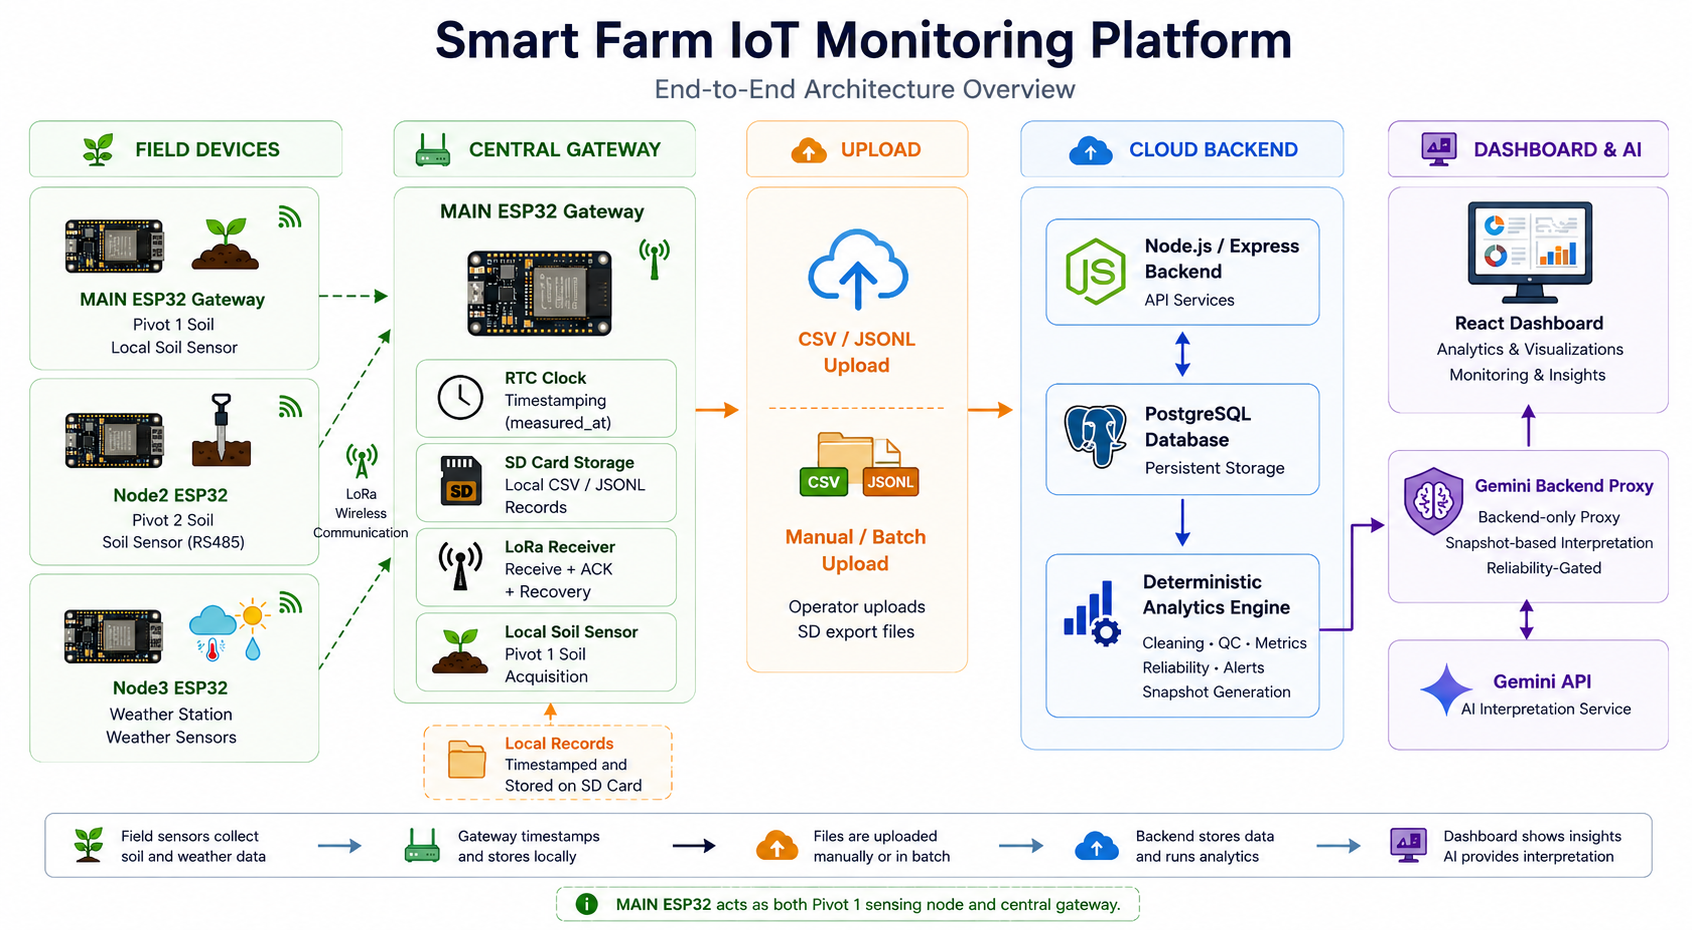
\includegraphics[width=\textwidth]{figures/overall-diagram}
% TODO: copy Academic-Thesis/Diagrams/overall diagram.png to figures/overall-diagram.png before compiling
\caption{Overall system architecture showing the three hardware nodes, LoRa wireless communication, SD-based local storage, and the cloud backend and dashboard layers.}
\label{fig:overall-system-architecture}
\end{figure}

The MAIN gateway node is the operational centre of the field tier. It coordinates the measurement cycle of all three nodes, maintains the authoritative real-time clock, manages SD card storage, and orchestrates data upload. Node2, a remote soil sensing unit deployed at the second irrigation pivot, acquires soil measurements and transmits them to MAIN via LoRa. Node3, a dedicated weather node, collects atmospheric parameters and transmits them independently over the same LoRa link. The three nodes operate within a structured superframe of ten-minute duration, during which each node executes its sensing task, transmits its packet, and returns to a low-power state.

When an Internet connection is made available, the operator activates Upload Mode by holding the MAIN gateway button. Stored SD records are transmitted in batch to the WebService backend, where they are ingested into a PostgreSQL database. The upload process preserves the RTC-derived measurement timestamp for every reading; the upload timestamp is stored separately as transfer audit metadata and is never used in place of the measurement time for any analytical purpose. This distinction, identified as a gap in related works reviewed in Chapter~\ref{chap:related-works}, is enforced at every layer of the implementation.

\begin{figure}[H]
\centering
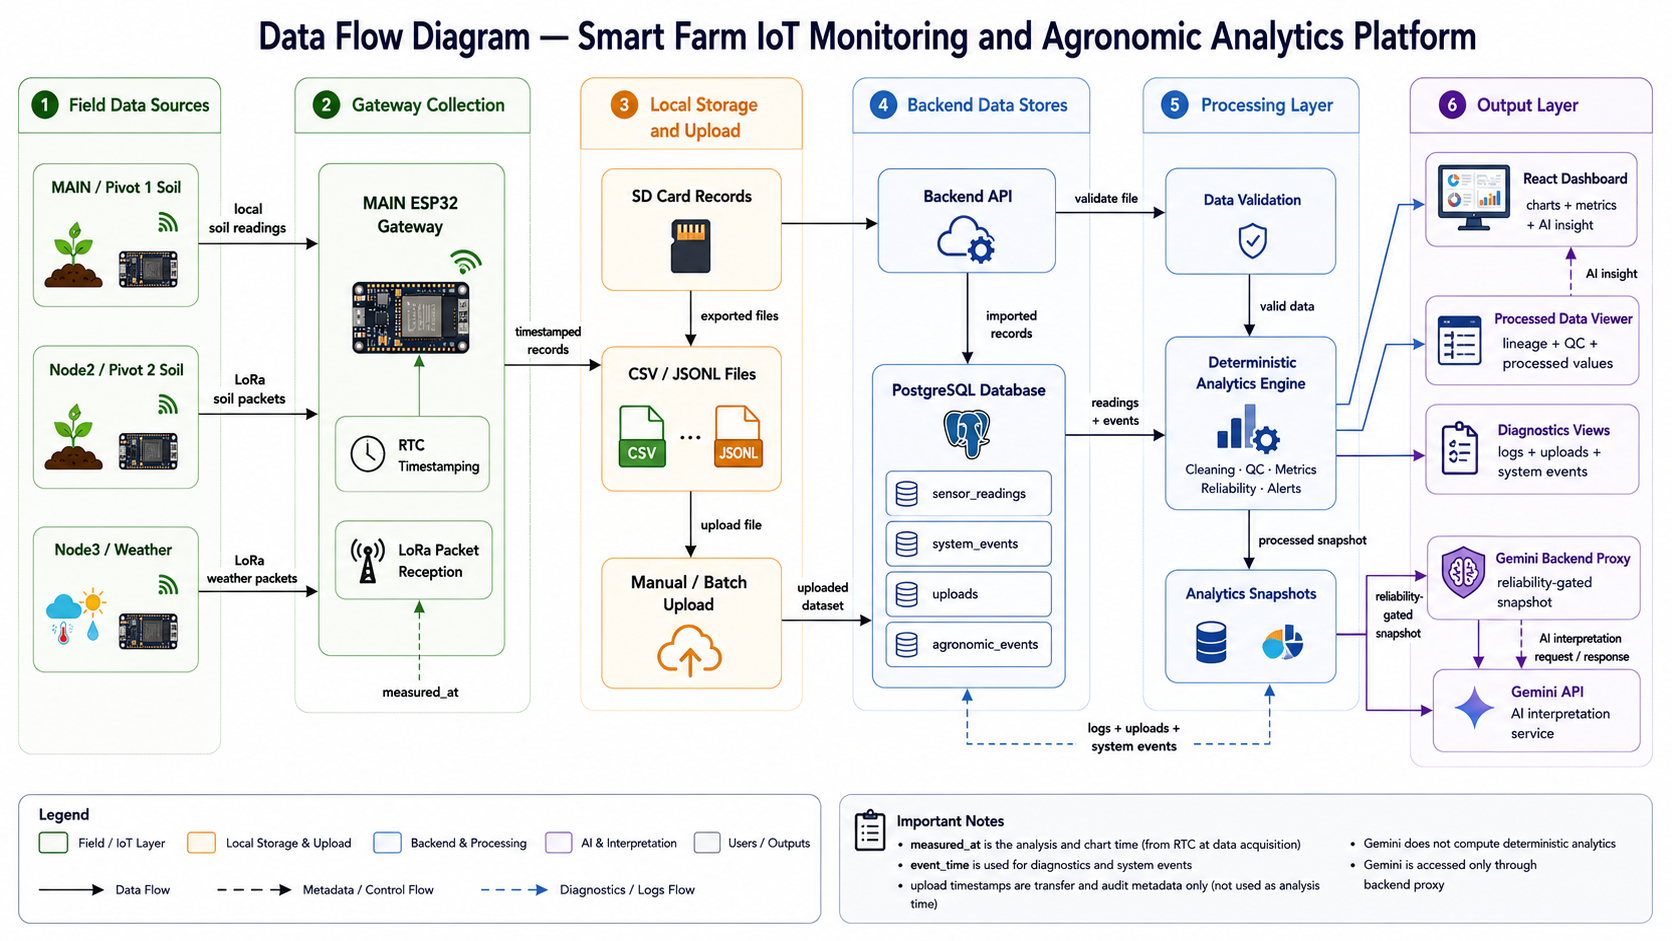
\includegraphics[width=\textwidth]{figures/data-flow-diagram}
% TODO: copy Academic-Thesis/Diagrams/Data Flow Diagram.png to figures/data-flow-diagram.png before compiling
\caption{Data flow diagram illustrating the movement of sensor readings from field acquisition through local storage, batch upload, backend ingestion, and dashboard presentation.}
\label{fig:data-flow-diagram}
\end{figure}

Figure~\ref{fig:data-flow-diagram} traces the complete data path from sensor to dashboard. All measurement data flows from sensors through the MAIN gateway, where it is timestamped and stored locally. Upload transfers SD content to the backend; the backend performs ingestion, validation, and analytics snapshot computation. The dashboard retrieves data through the backend API and presents readings, events, diagnostics, and analytics to the operator. At no stage in this flow does the upload timestamp overwrite or substitute for the RTC-derived measurement timestamp.

% ============================================================
\section{Hardware Architecture}
\label{sec:hardware}
% ============================================================

The system is composed of three hardware nodes, each serving a distinct role in the field monitoring architecture. Table~\ref{tab:node-roles} summarises the roles and primary responsibilities of each node.

\begin{table}[H]
\centering
\caption{Summary of node roles in the system architecture.}
\label{tab:node-roles}
\small
\begin{tabular}{p{2.5cm} p{3.0cm} p{4.0cm} p{4.5cm}}
\hline
\textbf{Node} & \textbf{Microcontroller} & \textbf{Primary function} & \textbf{Location} \\
\hline
MAIN gateway & ESP32 38-pin & Coordination, Pivot~1 soil sensing, RTC, SD storage, upload & Field base station (Pivot~1 location) \\
\hline
Node2 & ESP32-C3 Super Mini & Pivot~2 soil sensing, LoRa transmission & Pivot~2 location (remote) \\
\hline
Node3 & ESP32-C3 Super Mini & Weather monitoring, LoRa transmission & Field weather station position \\
\hline
\end{tabular}
\end{table}

% ----------------------------------------------------------
\subsection{MAIN ESP32 Gateway Node}
\label{sec:main-node}
% ----------------------------------------------------------

The MAIN node is an ESP32 38-pin development board that serves as the operational centre of the field sensing network. It performs four distinct functions within each measurement cycle: it opens a LoRa receive window to collect packets from Node2 and Node3, it reads the local soil sensor at Pivot~1 via RS485/Modbus, it writes all acquired readings and events to the SD card, and it manages upload and RTC synchronisation when requested by the operator.

\begin{figure}[H]
\centering
\begin{minipage}[b]{0.48\textwidth}
\centering
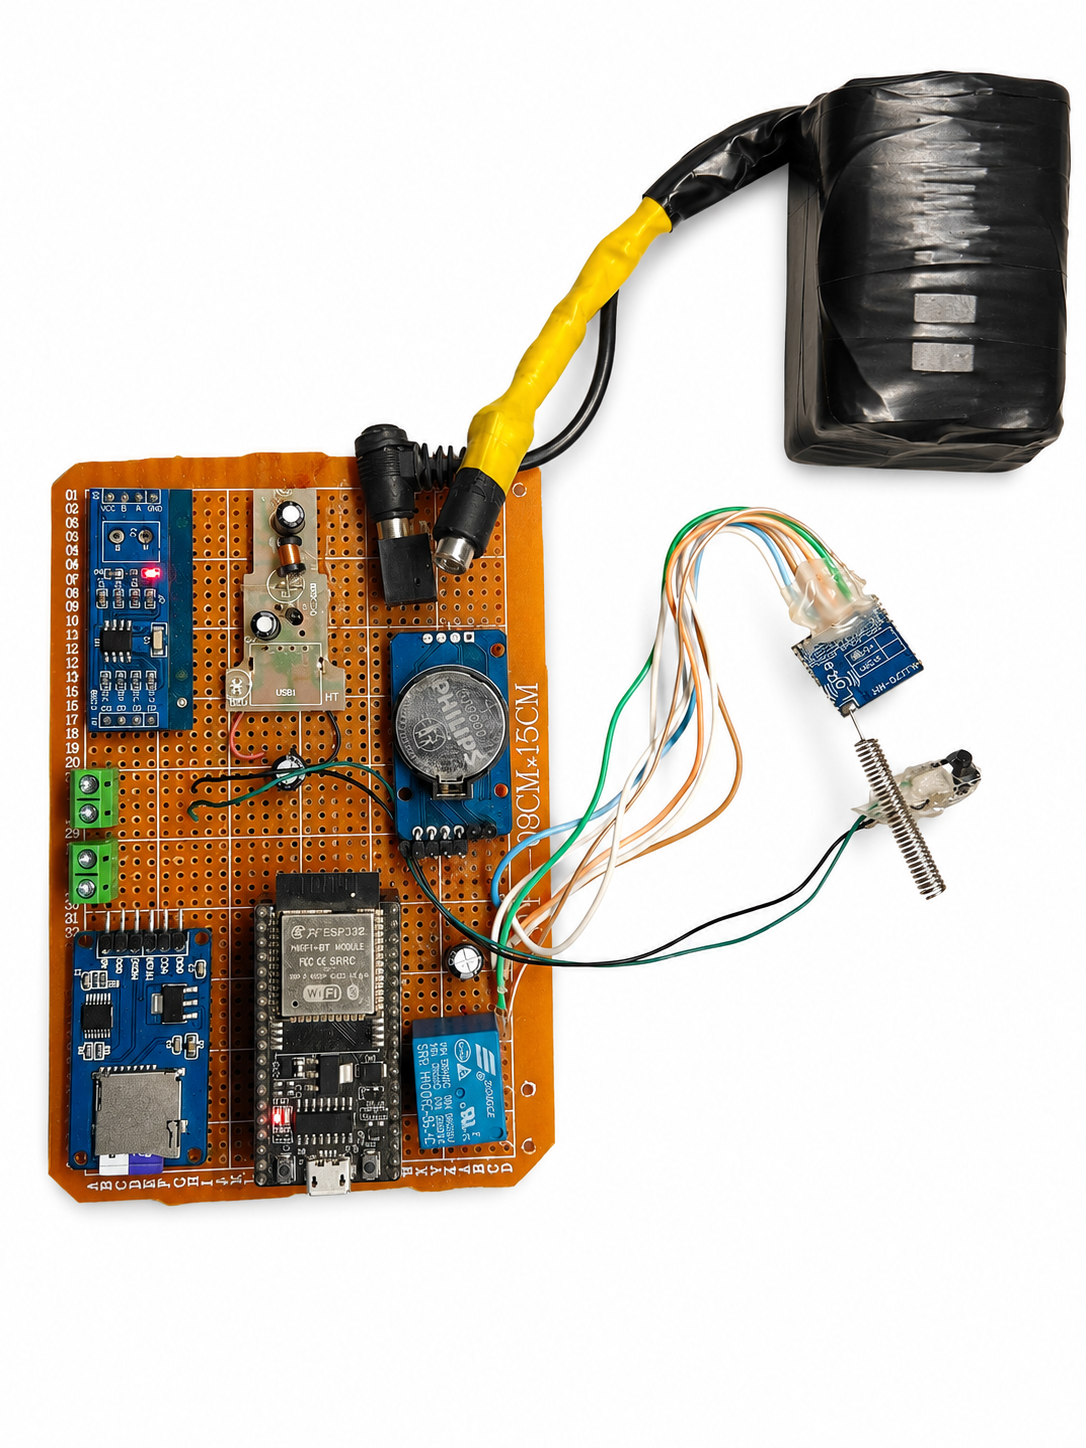
\includegraphics[width=\textwidth]{figures/MainNodeFront}
% TODO: copy Academic-Thesis/SystemImage/MainNodeFront.png to figures/MainNodeFront.png before compiling
\caption{MAIN gateway node — front view showing the ESP32 board, RTC module, and LoRa transceiver.}
\label{fig:main-node-front}
\end{minipage}
\hfill
\begin{minipage}[b]{0.48\textwidth}
\centering
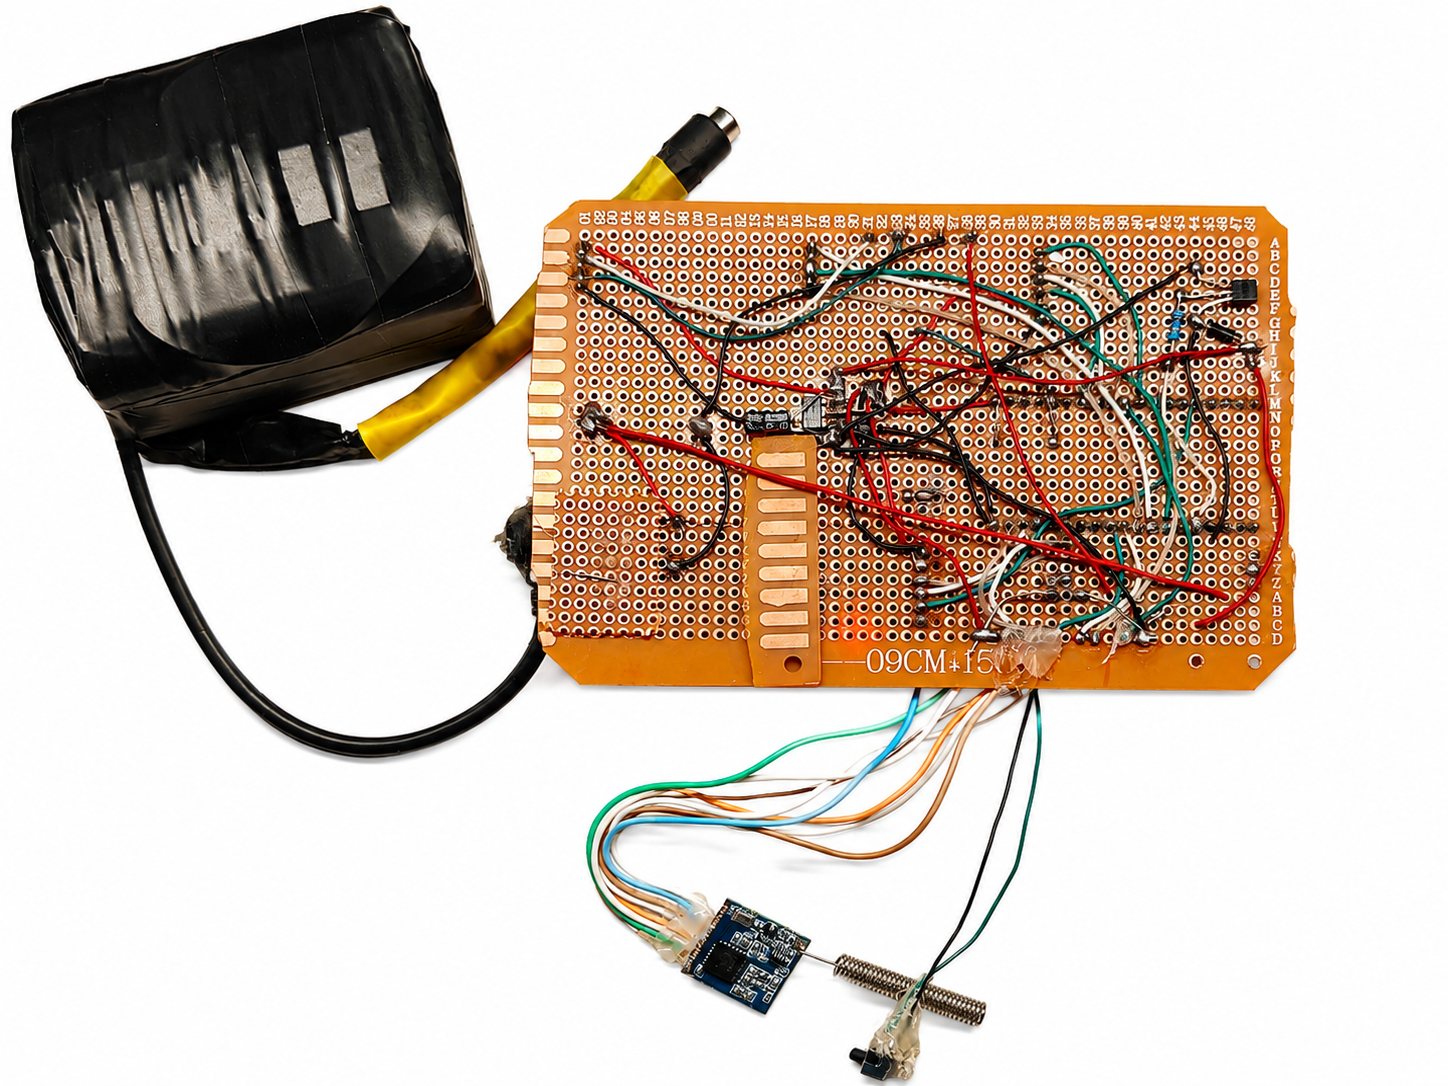
\includegraphics[width=\textwidth]{figures/MainNodeBack}
% TODO: copy Academic-Thesis/SystemImage/MainNodeBack.png to figures/MainNodeBack.png before compiling
\caption{MAIN gateway node — rear view showing the SD card module and wiring connections.}
\label{fig:main-node-back}
\end{minipage}
\end{figure}

\begin{figure}[H]
\centering
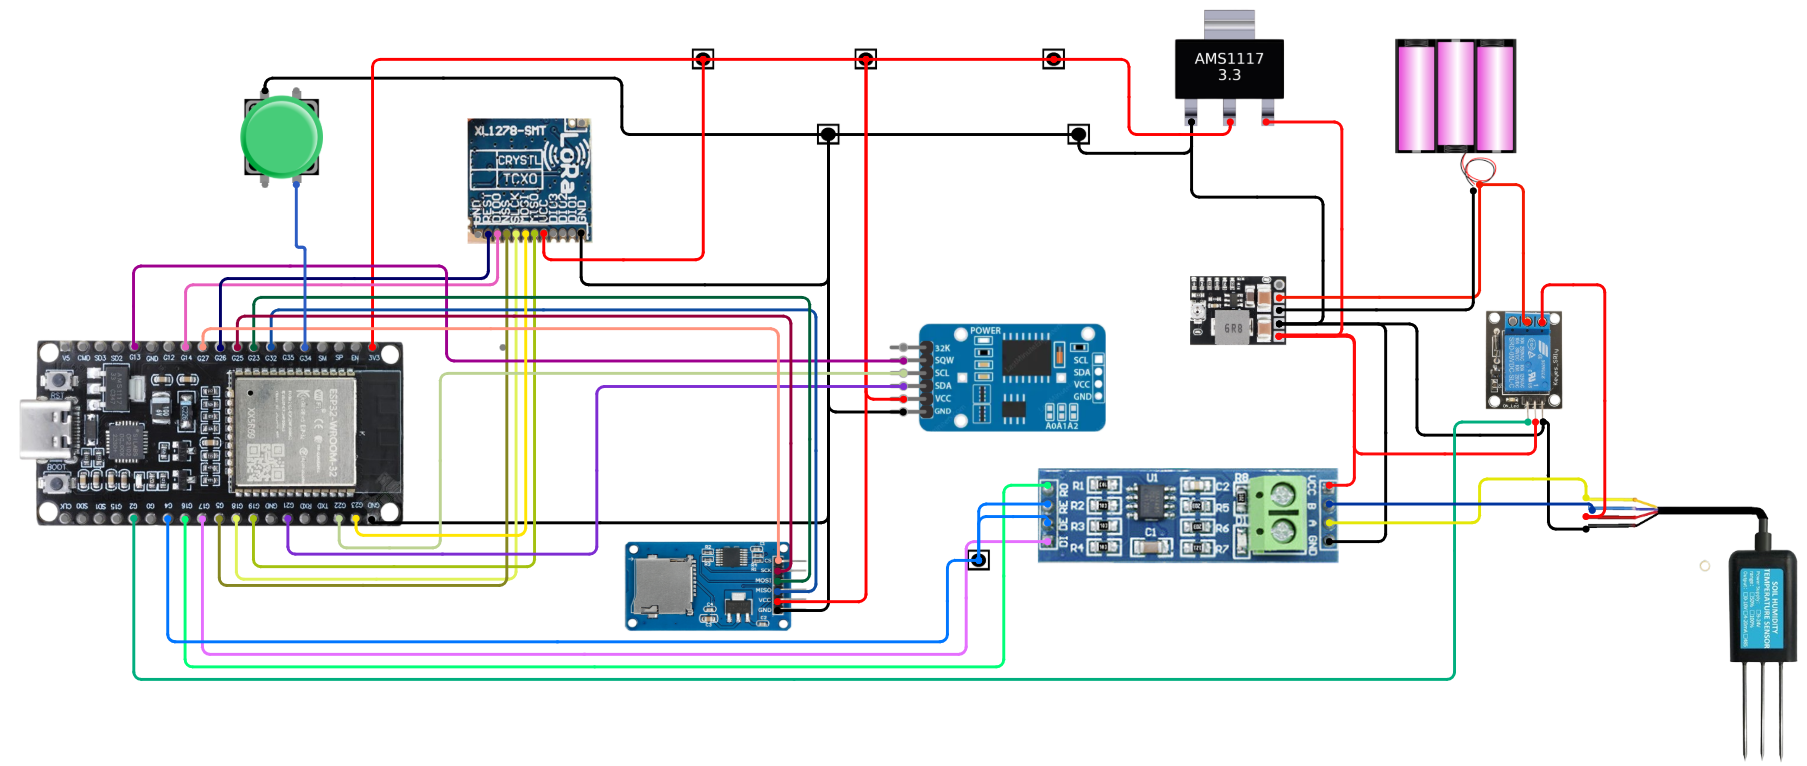
\includegraphics[width=0.85\textwidth]{figures/MainNodeWiringDiagram}
% TODO: copy Academic-Thesis/Diagrams/MainNodeWiringDiagram.png to figures/MainNodeWiringDiagram.png before compiling
\caption{MAIN gateway node wiring diagram showing pin connections between the ESP32, DS3231 RTC, SD card module, SX127x LoRa transceiver, MAX485 RS485 interface, and relay module.}
\label{fig:main-node-wiring}
\end{figure}

The MAIN node integrates five hardware subsystems. The DS3231 RTC module, connected over I2C (SDA\,=\,GPIO21, SCL\,=\,GPIO22), provides the authoritative measurement timestamp. A dedicated SPI bus (VSPI: MISO\,=\,GPIO19, MOSI\,=\,GPIO23, SCK\,=\,GPIO18, CS\,=\,GPIO5, RST\,=\,GPIO26, DIO0\,=\,GPIO14) connects the SX127x LoRa transceiver for wireless reception from remote nodes. A second SPI bus (HSPI: MISO\,=\,GPIO32, MOSI\,=\,GPIO33, SCK\,=\,GPIO25, CS\,=\,GPIO27) connects the SD card module for local data persistence. A MAX485 RS485 transceiver and relay module serve the local Pivot~1 soil sensor; the relay is used to control sensor power and is switched on immediately before a measurement and switched off immediately after, regardless of whether the read succeeds.

\begin{figure}[H]
\centering
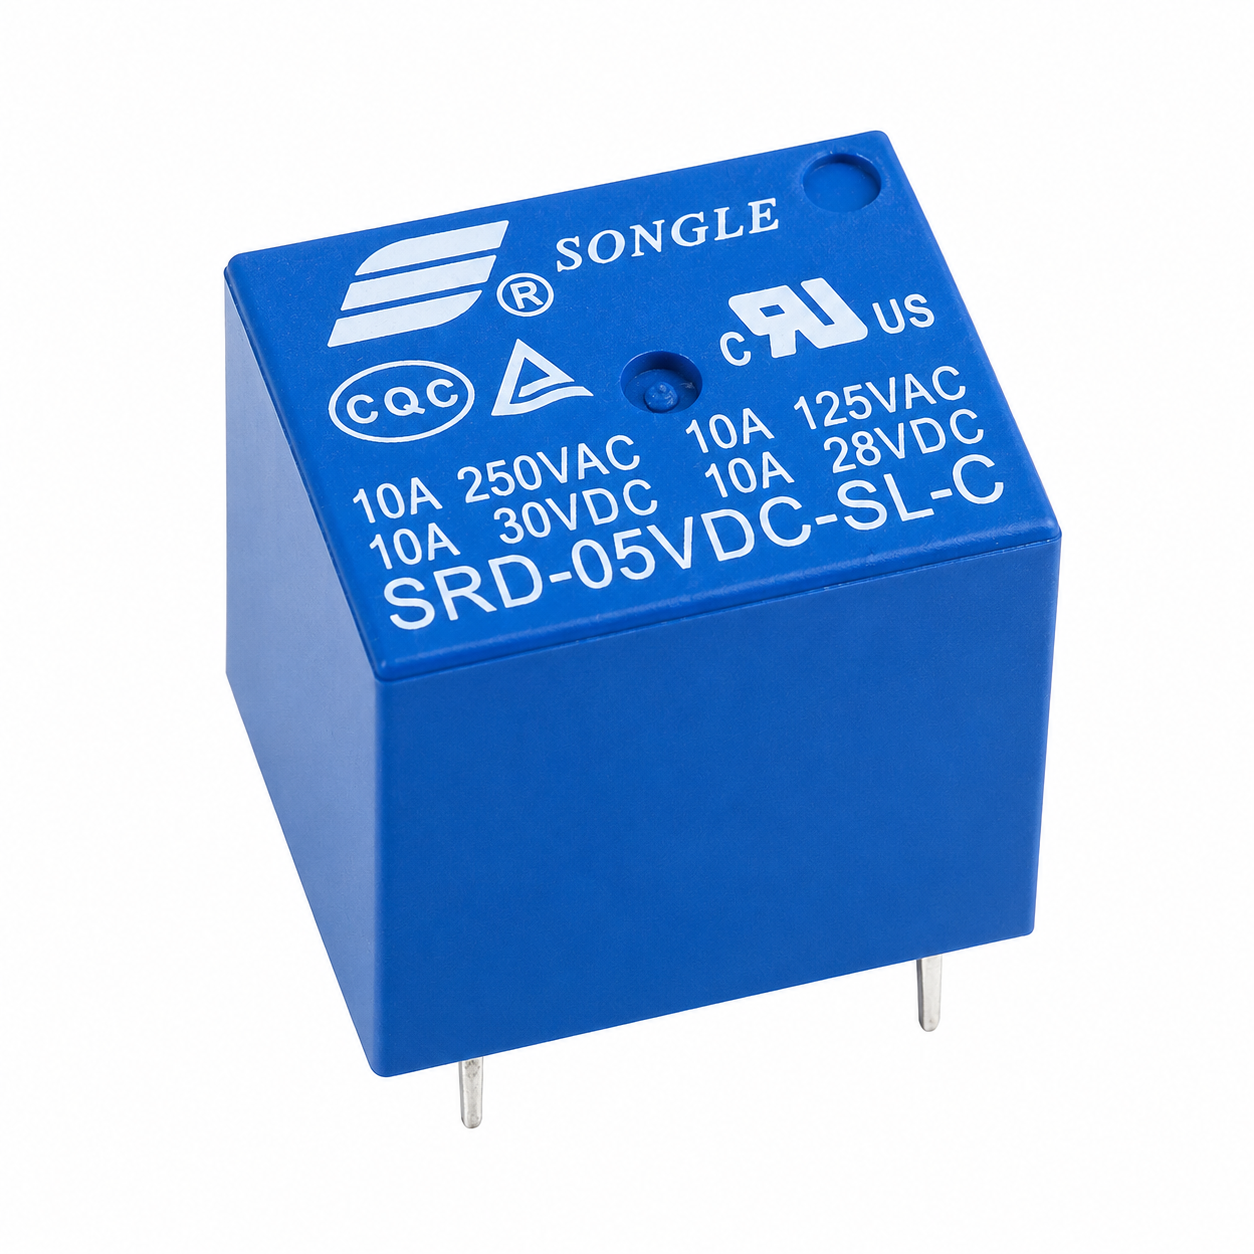
\includegraphics[width=0.35\textwidth]{figures/Relay}
% TODO: copy Academic-Thesis/SystemImage/Relay.png to figures/Relay.png before compiling
\caption{Relay module used on the MAIN node and Node2 to control RS485 soil sensor power. The relay is activated for the duration of the sensor warmup and read sequence and deactivated immediately after to minimise continuous current draw.}
\label{fig:relay-module-ch3}
\end{figure}

The Pivot~1 local soil sensor is interfaced over RS485 using Modbus RTU at 4800~baud, 8N1, with slave address 0x01, function code 0x03, and three registers beginning at address 0x0000, yielding soil moisture (tenths of a percent), soil temperature (tenths of a degree Celsius), and soil EC (integer, µS/cm). The firmware activates the relay, waits 15~seconds for sensor warm-up, issues the Modbus query, then deactivates the relay. During the validation period documented in Part~B, the Modbus register map for the Pivot~1 sensor was not yet finalised in the firmware; the \texttt{performLocalSoilMeasurement()} routine completes the relay control sequence on each cycle, but the register read returns a \texttt{LOCAL\_SOIL\_REGISTER\_MAP\_MISSING} diagnostic code rather than measured values. This state is reflected accurately in the validation evidence. The Pivot~1 hardware path is fully wired and the firmware structure is in place; the register map will be confirmed when the sensor's Modbus documentation is verified against the installed unit.

A push-button on GPIO34 provides the operator interface for Upload Mode and RTC Synchronisation Mode. A long press (sustained contact of one second or more) triggers batch upload of SD content. Four consecutive short presses trigger RTC synchronisation. The MAIN node does not expose a network interface during normal sensing cycles; network activity occurs only during Upload Mode.

% ----------------------------------------------------------
\subsection{Node2 Remote Soil Node}
\label{sec:node2}
% ----------------------------------------------------------

Node2 is an ESP32-C3 Super Mini development board deployed at the Pivot~2 location, physically separated from the MAIN gateway. Its sole sensing responsibility is the acquisition of soil moisture, temperature, and EC from the soil sensor installed at Pivot~2. Because Pivot~1 and Pivot~2 represent distinct irrigation zones with independent soil conditions, the two soil data streams are complementary rather than redundant.

\begin{figure}[H]
\centering
\begin{minipage}[b]{0.48\textwidth}
\centering
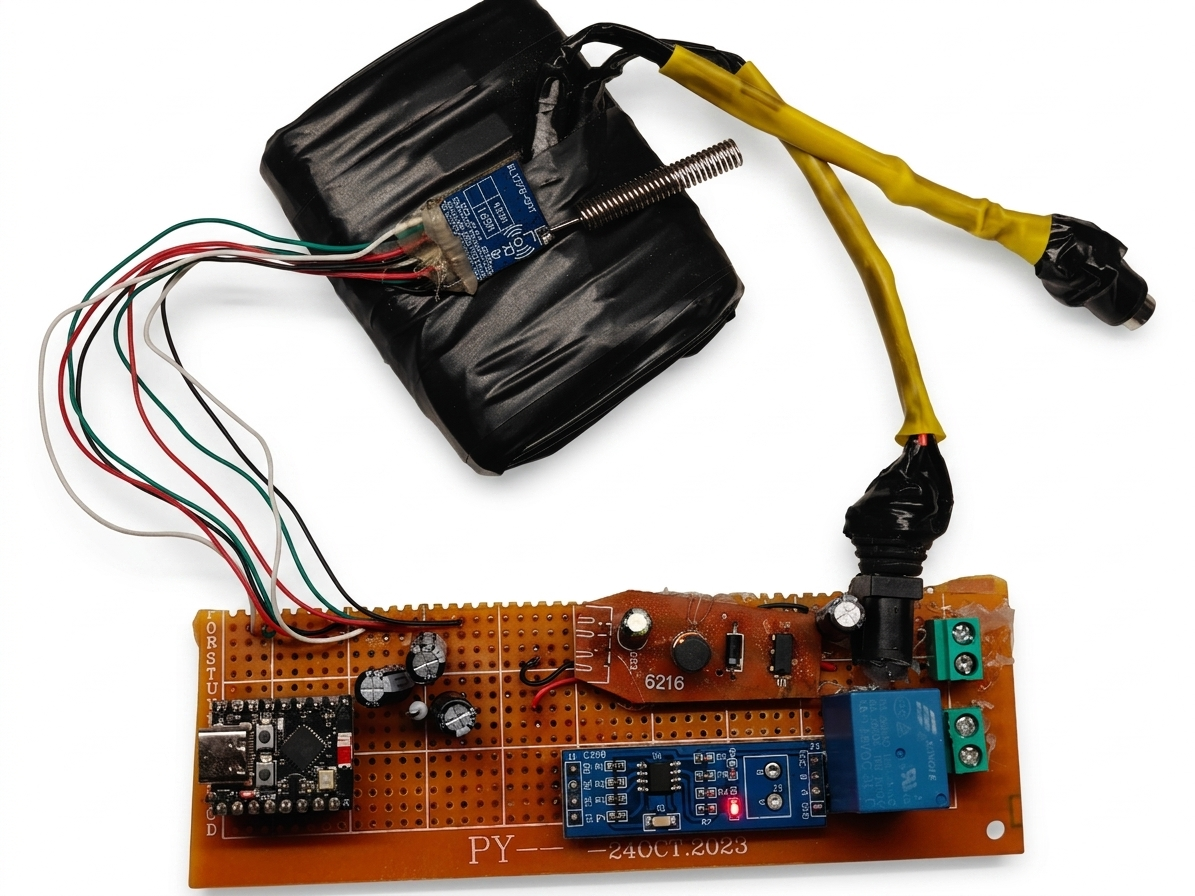
\includegraphics[width=\textwidth]{figures/SecondNodeFront}
% TODO: copy Academic-Thesis/SystemImage/SecondNodeFront.png to figures/SecondNodeFront.png before compiling
\caption{Node2 soil node — front view showing the ESP32-C3 board and LoRa module.}
\label{fig:node2-front}
\end{minipage}
\hfill
\begin{minipage}[b]{0.48\textwidth}
\centering
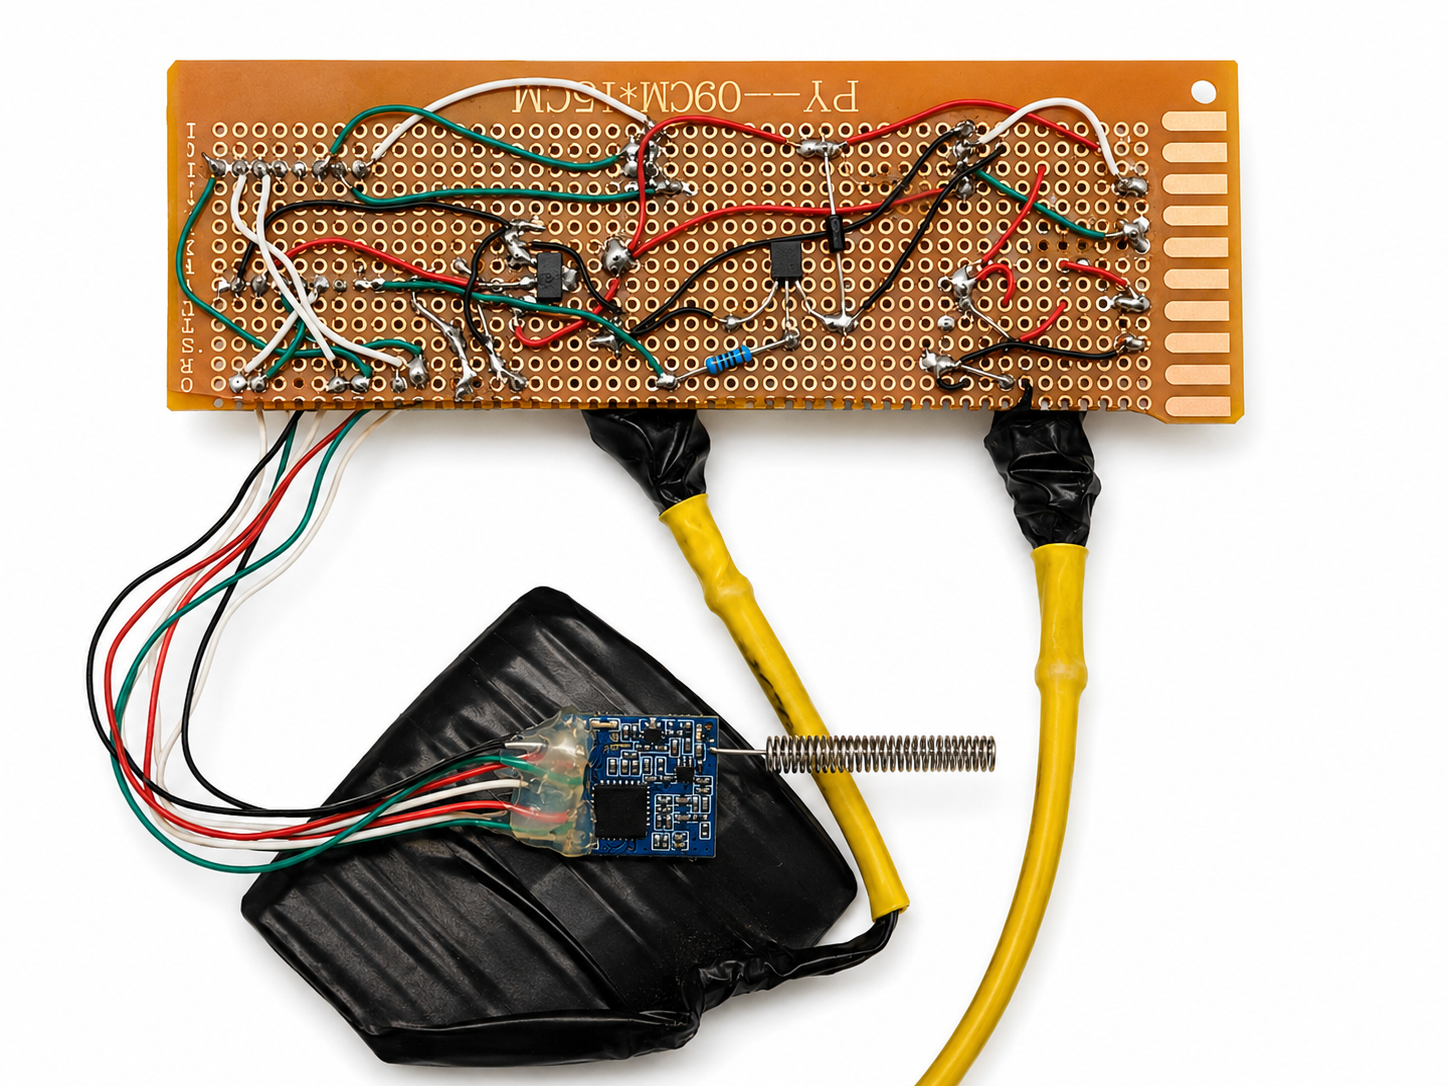
\includegraphics[width=\textwidth]{figures/SecondNodeBack}
% TODO: copy Academic-Thesis/SystemImage/SecondNodeBack.png to figures/SecondNodeBack.png before compiling
\caption{Node2 soil node — rear view showing the MAX485 interface and relay wiring.}
\label{fig:node2-back}
\end{minipage}
\end{figure}

\begin{figure}[H]
\centering
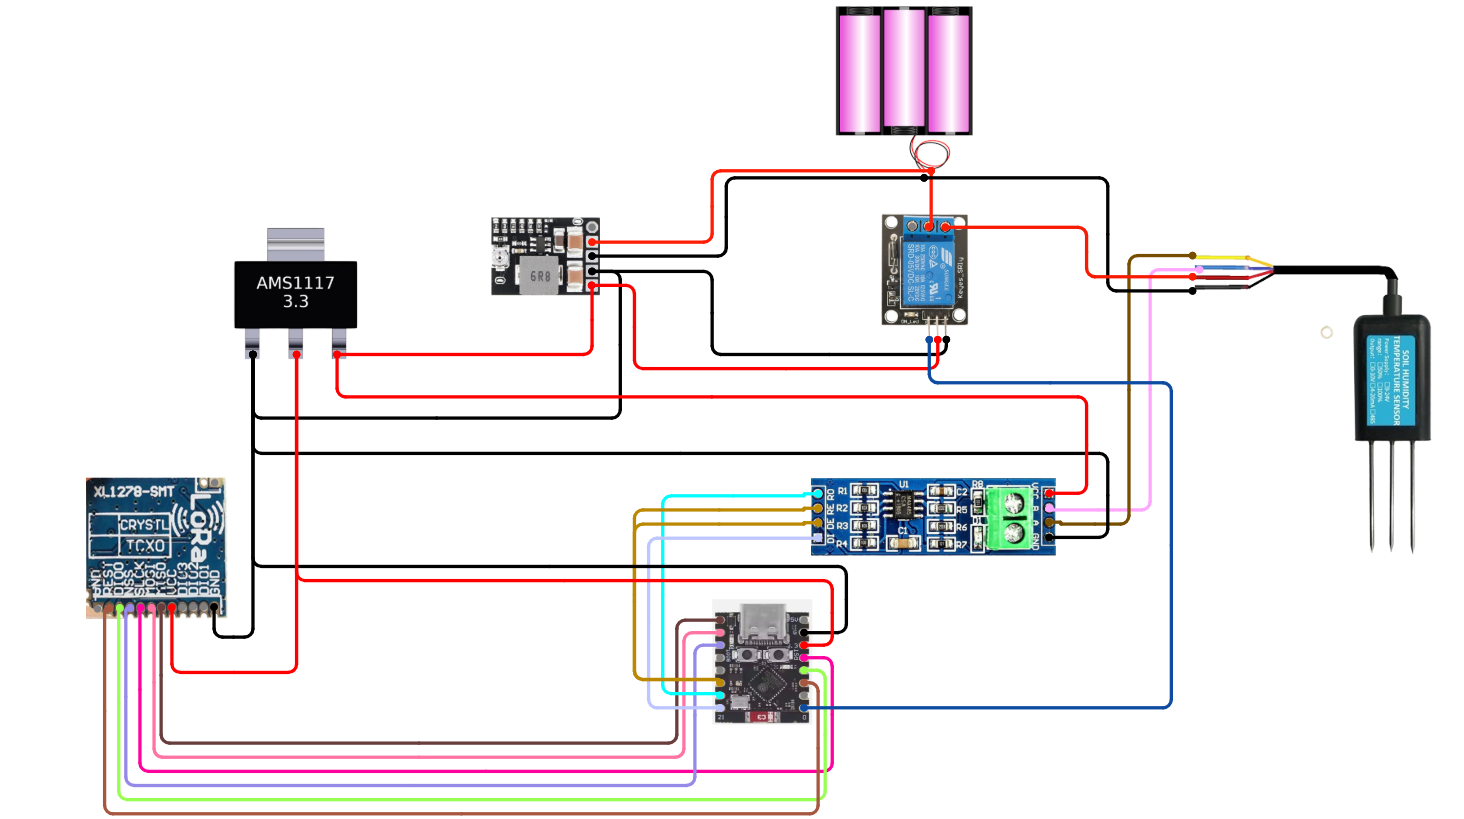
\includegraphics[width=0.85\textwidth]{figures/Node2WiringDiagram}
% TODO: copy Academic-Thesis/Diagrams/Node2WiringDiagram.png to figures/Node2WiringDiagram.png before compiling
\caption{Node2 wiring diagram showing pin connections between the ESP32-C3, SX127x LoRa transceiver, MAX485 RS485 interface, relay module, and RS485 soil sensor.}
\label{fig:node2-wiring}
\end{figure}

The LoRa transceiver is connected to the ESP32-C3 SPI bus (SCK\,=\,GPIO4, MISO\,=\,GPIO5, MOSI\,=\,GPIO6, CS\,=\,GPIO7, RST\,=\,GPIO2, DIO0\,=\,GPIO3). The MAX485 RS485 transceiver uses GPIO10 for the direction control (DE/RE combined), GPIO20 for the receive line (RO), and GPIO21 for the transmit line (DI). A relay on GPIO0 controls power to the RS485 soil sensor, applying the same relay-on, warm-up, read, relay-off sequence used on the MAIN node.

\begin{figure}[H]
\centering
\begin{minipage}[b]{0.45\textwidth}
\centering
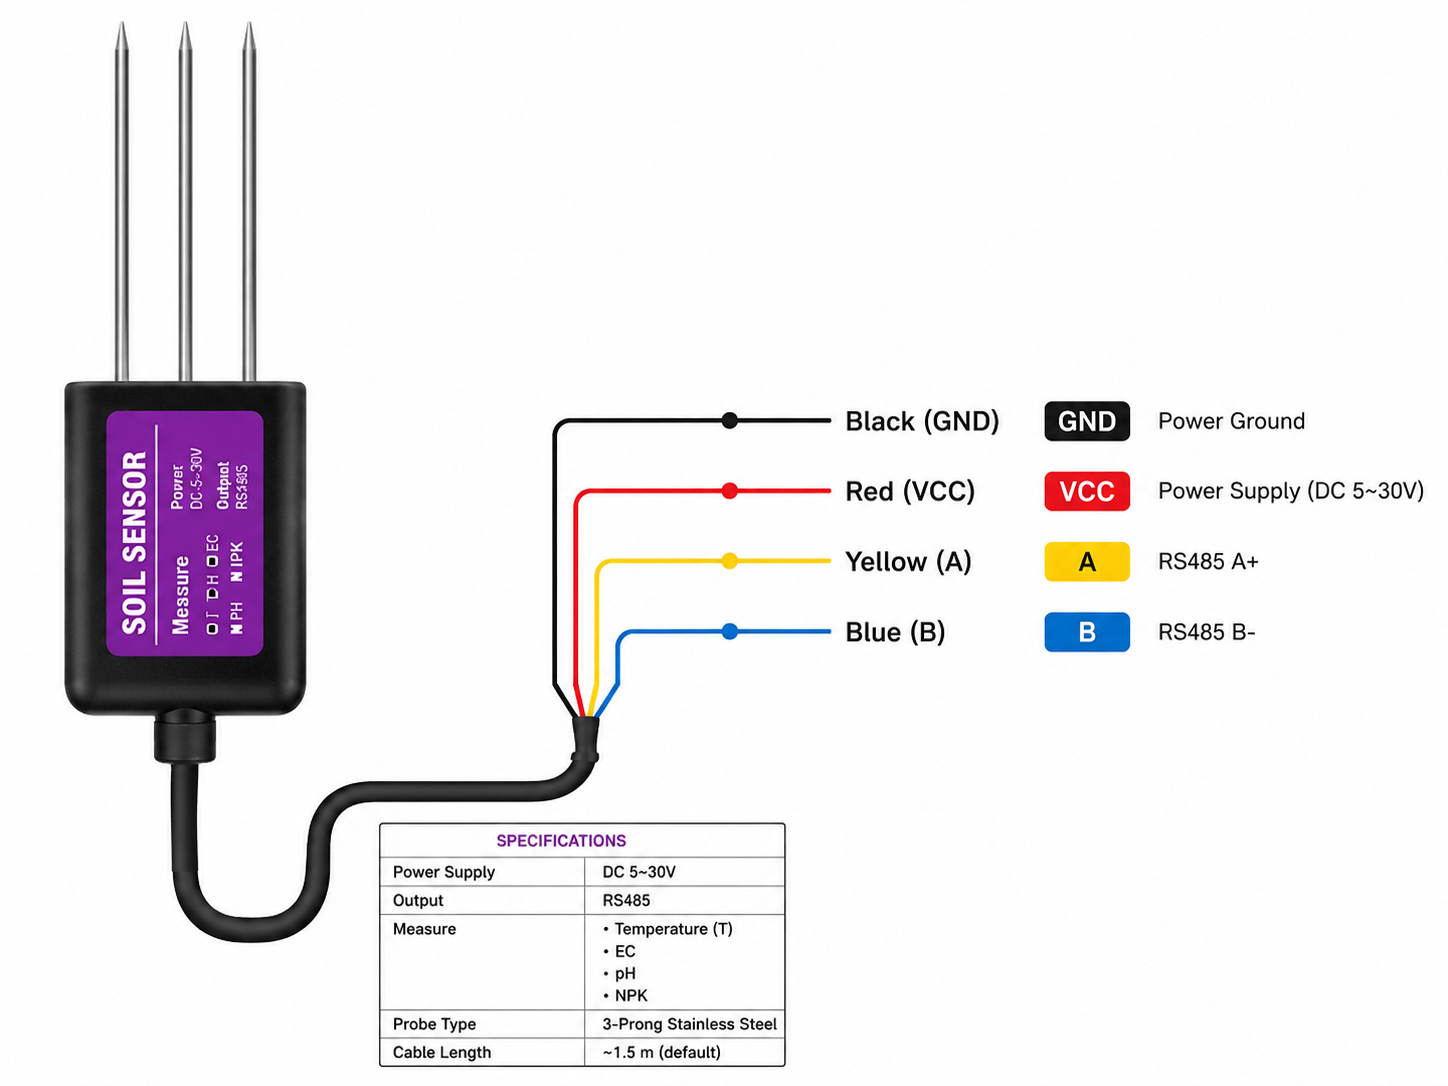
\includegraphics[width=\textwidth]{figures/SoilSensor}
% TODO: copy Academic-Thesis/SystemImage/SoilSensor.png to figures/SoilSensor.png before compiling
\caption{RS485 soil sensor measuring moisture, temperature, and EC. The sensor is shared in design between the MAIN local (Pivot~1) and Node2 remote (Pivot~2) installations.}
\label{fig:soil-sensor}
\end{minipage}
\hfill
\begin{minipage}[b]{0.45\textwidth}
\centering
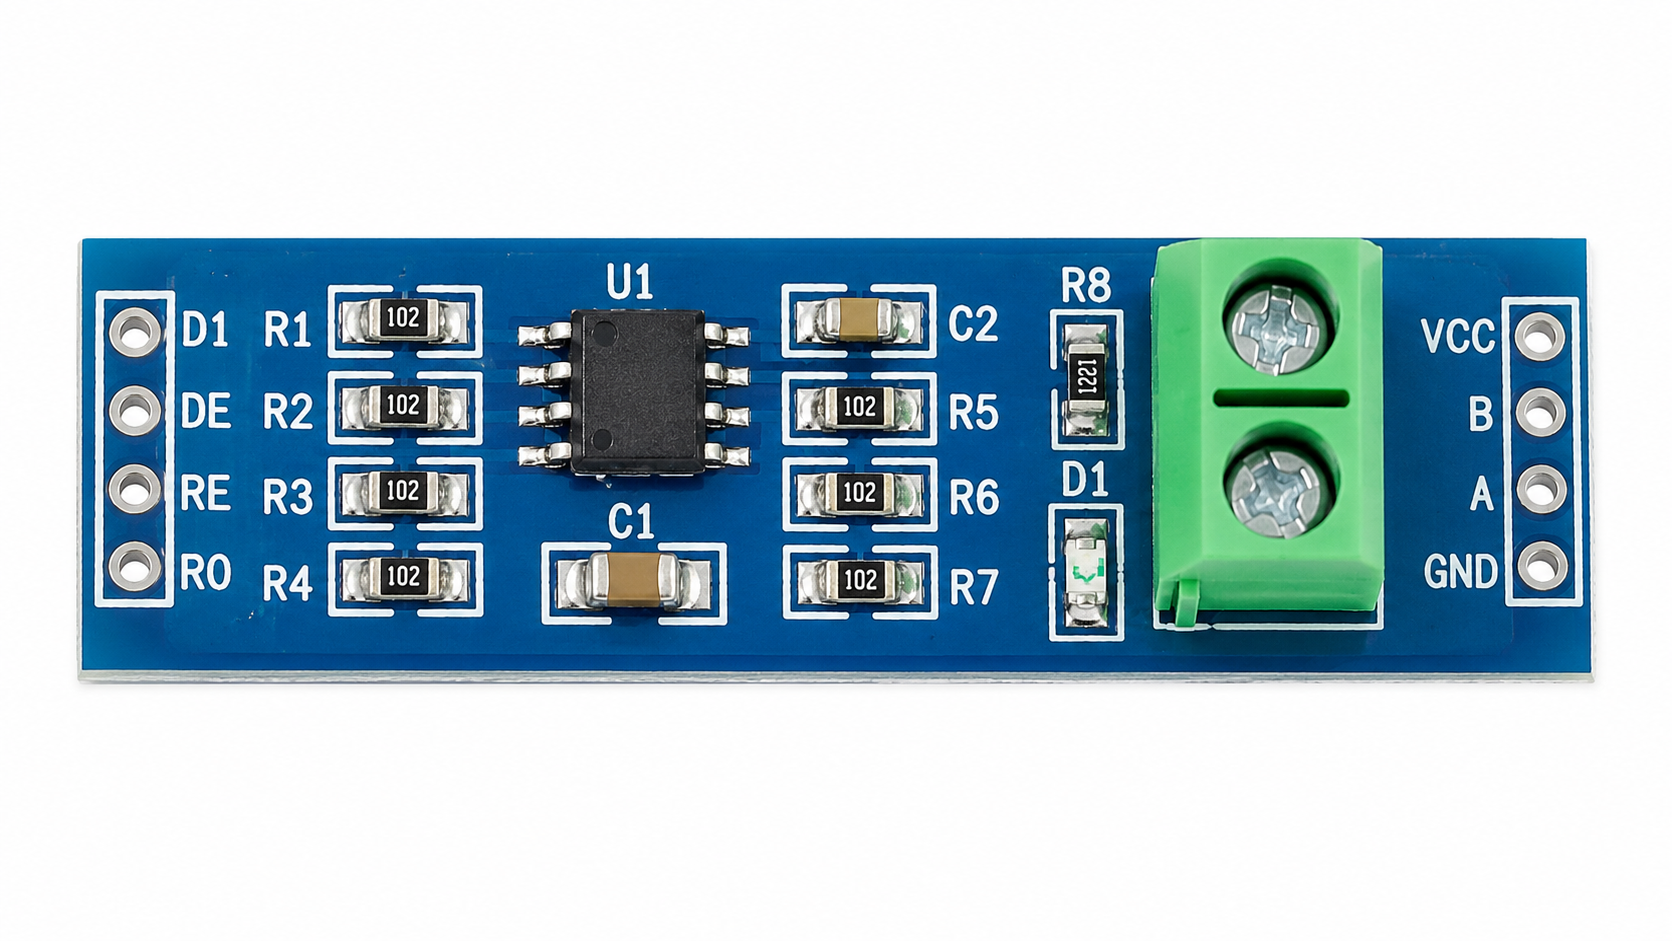
\includegraphics[width=\textwidth]{figures/Max485}
% TODO: copy Academic-Thesis/SystemImage/Max485.png to figures/Max485.png before compiling
\caption{MAX485 RS485 transceiver module used on both the MAIN node and Node2 for half-duplex serial communication with the Modbus soil sensor.}
\label{fig:max485}
\end{minipage}
\end{figure}

After completing its measurement, Node2 encodes the three sensor values into a LoRa packet and transmits at 433~MHz, spreading factor SF7, bandwidth 125~kHz, coding rate 4/5, with CRC enabled and a transmit power of 14~dBm. Node2 then enters deep sleep, with an interrupt scheduled to fire at the next transmission slot within the ten-minute superframe. The deep sleep interval is the primary mechanism by which Node2 conserves battery energy between measurement cycles.

% ----------------------------------------------------------
\subsection{Node3 Weather Node}
\label{sec:node3}
% ----------------------------------------------------------

Node3 is a second ESP32-C3 Super Mini, deployed as a dedicated atmospheric monitoring station. It measures air temperature, relative humidity, and barometric pressure using a BME280 sensor connected over I2C (SDA\,=\,GPIO8, SCL\,=\,GPIO9). The LoRa transceiver uses the same SPI pin assignment as Node2 (SCK\,=\,GPIO4, MISO\,=\,GPIO5, MOSI\,=\,GPIO6, CS\,=\,GPIO7, RST\,=\,GPIO2, DIO0\,=\,GPIO3).

\begin{figure}[H]
\centering
\begin{minipage}[b]{0.48\textwidth}
\centering
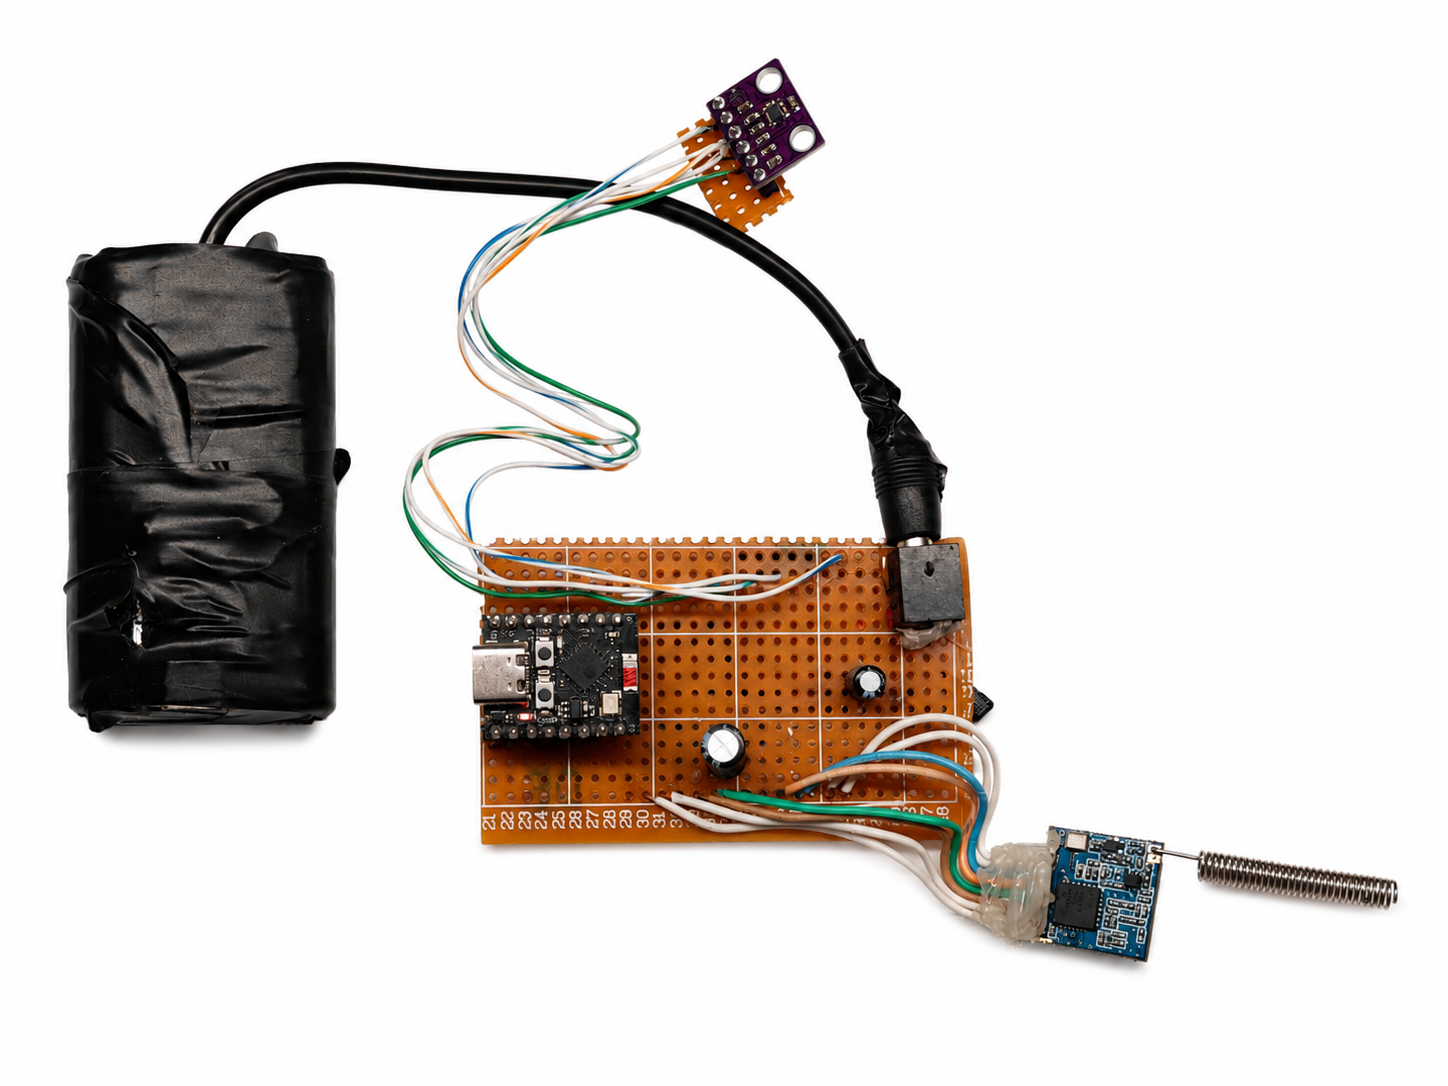
\includegraphics[width=\textwidth]{figures/WatherNodeFront}
% TODO: rename WatherNodeFront.png to WeatherNodeFront.png in Academic-Thesis/SystemImage/ for consistency; copy to figures/WatherNodeFront.png before compiling
\caption{Node3 weather node — front view showing the ESP32-C3 board, BME280 sensor, and LoRa module.}
\label{fig:node3-front}
\end{minipage}
\hfill
\begin{minipage}[b]{0.48\textwidth}
\centering
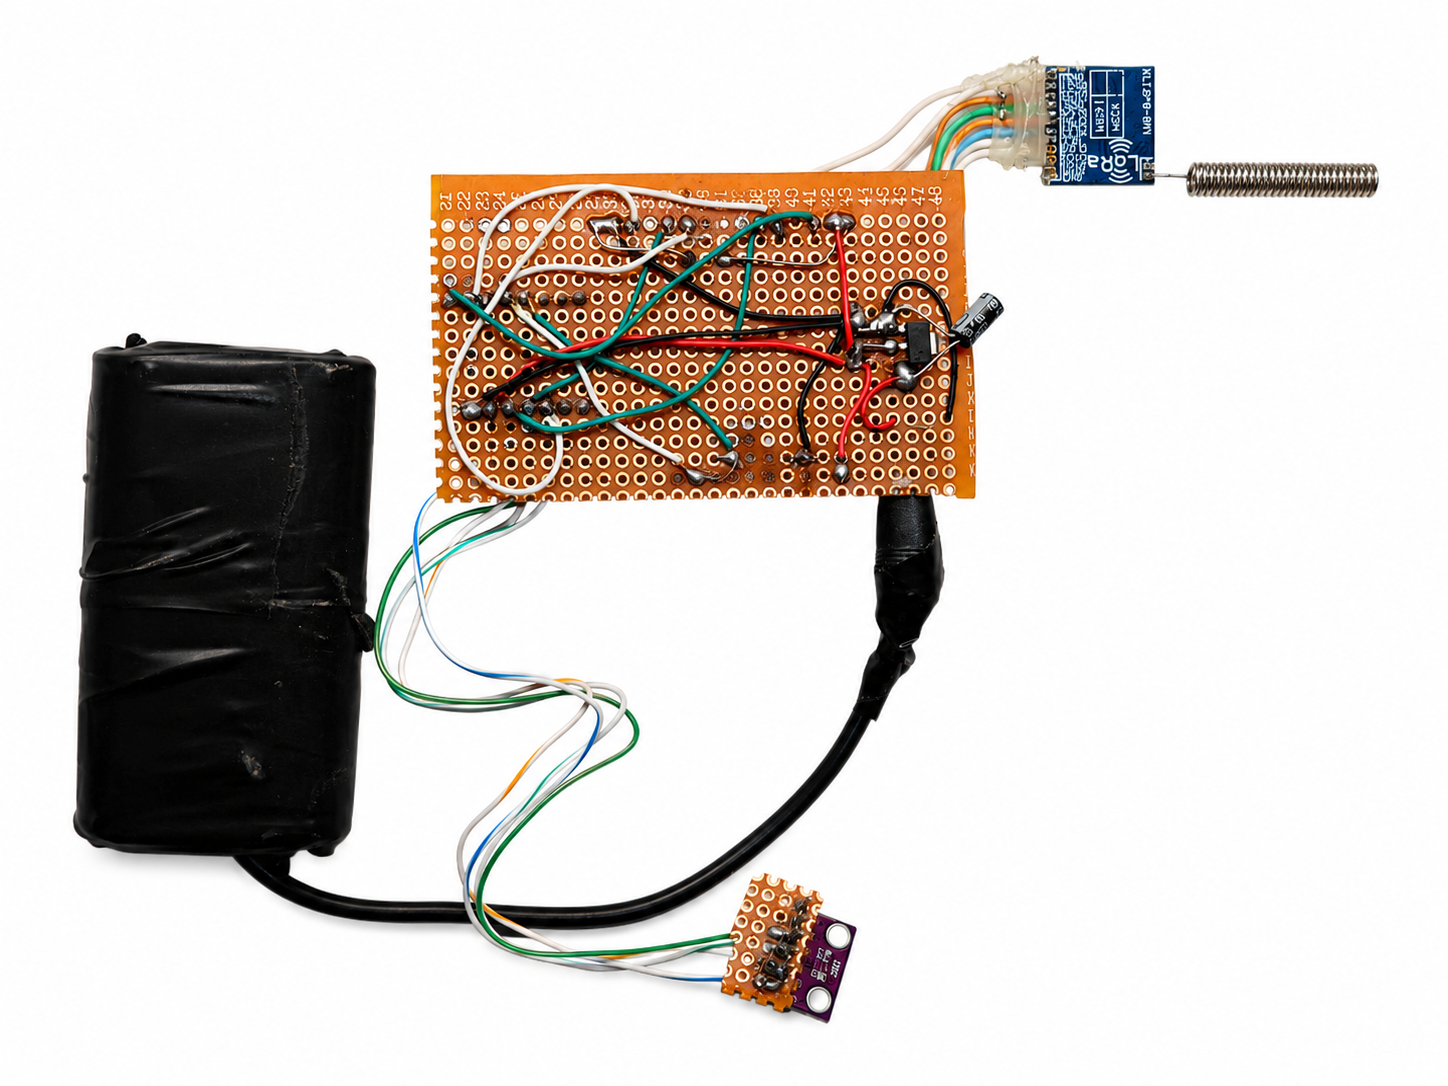
\includegraphics[width=\textwidth]{figures/WatherNodeBack}
% TODO: rename WatherNodeBack.png to WeatherNodeBack.png in Academic-Thesis/SystemImage/ for consistency; copy to figures/WatherNodeBack.png before compiling
\caption{Node3 weather node — rear view showing the I2C connections to the BME280 module.}
\label{fig:node3-back}
\end{minipage}
\end{figure}

\begin{figure}[H]
\centering
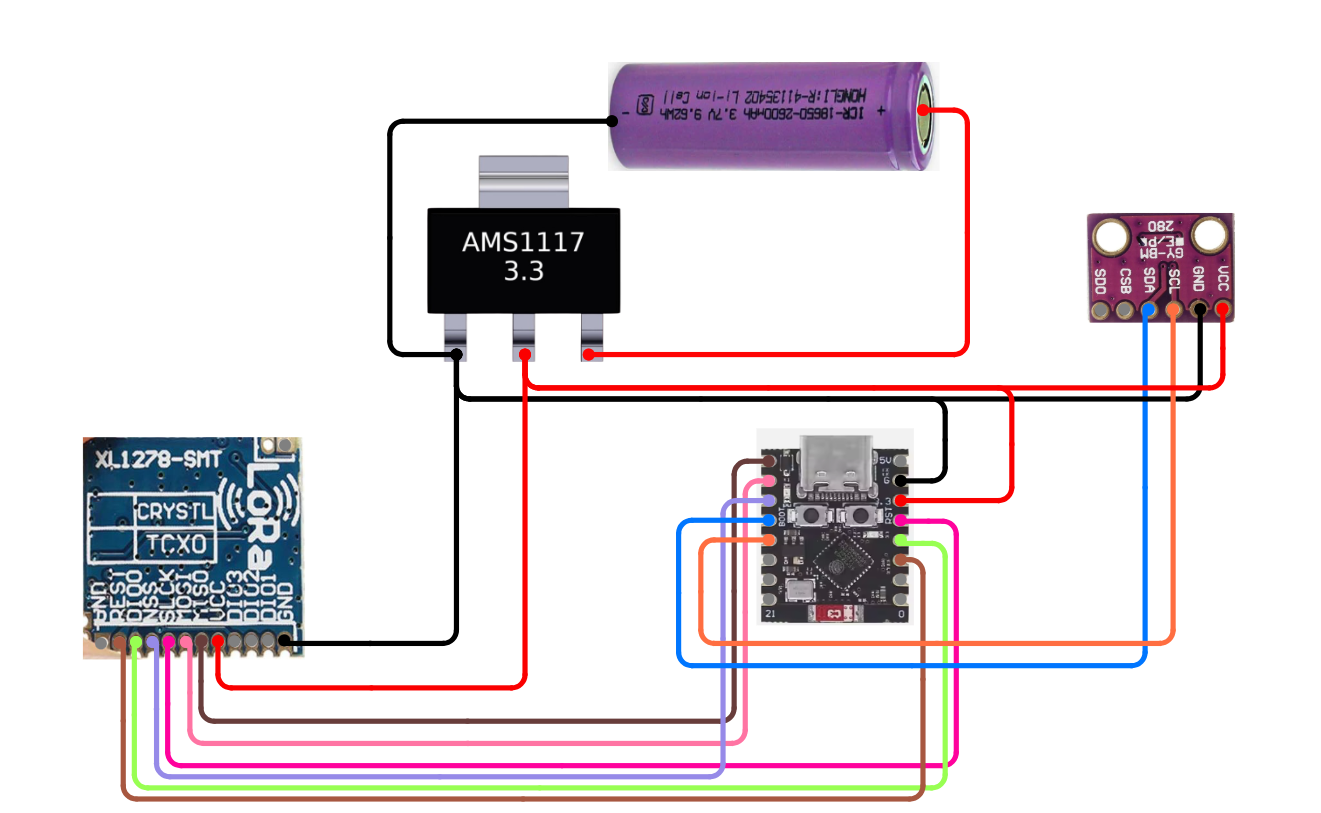
\includegraphics[width=0.85\textwidth]{figures/WatherNodeWiringDiagram}
% TODO: rename WatherNodeWiringDiagram.png to WeatherNodeWiringDiagram.png in Academic-Thesis/Diagrams/ for consistency; copy to figures/WatherNodeWiringDiagram.png before compiling
\caption{Node3 weather node wiring diagram showing connections between the ESP32-C3, BME280 environmental sensor (I2C), and SX127x LoRa transceiver (SPI).}
\label{fig:node3-wiring}
\end{figure}

The BME280 is operated in forced measurement mode, a single-shot acquisition pattern in which the sensor is commanded to take one reading, delivers the result, and returns to sleep mode automatically. This eliminates the continuous power draw that would result from leaving the sensor in normal (continuous) mode. The active measurement window per cycle is under two seconds, after which Node3 encodes its three atmospheric values, transmits the LoRa packet, and returns to deep sleep. No relay is required for Node3 because the BME280's own forced-mode power management is sufficient.

\begin{figure}[H]
\centering
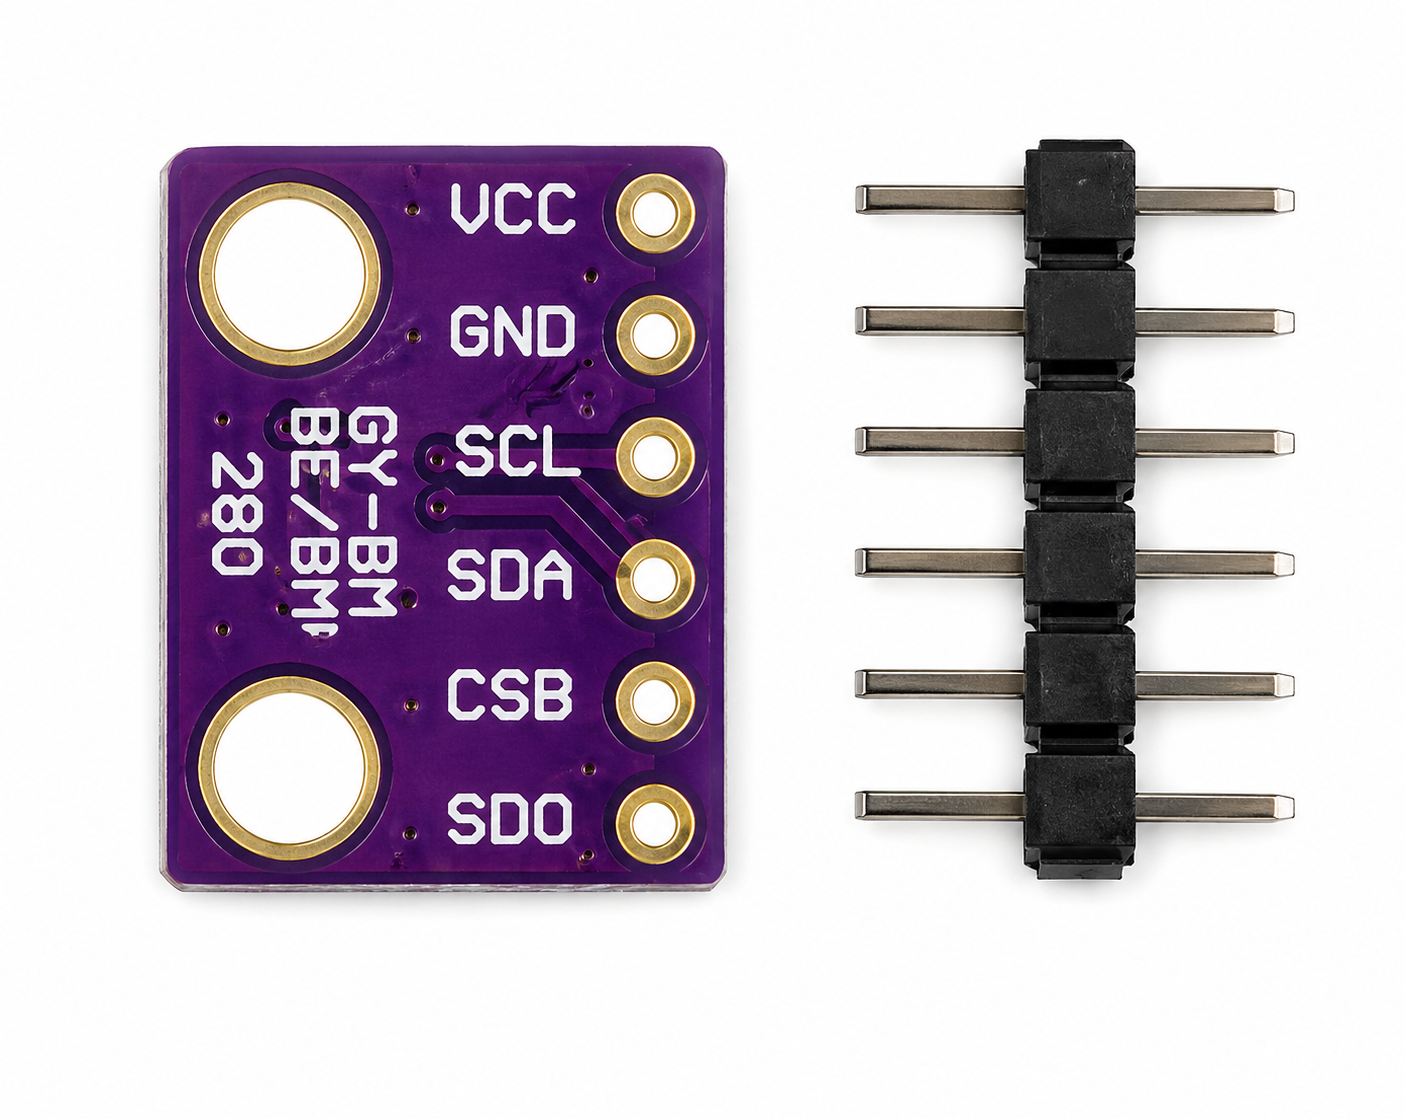
\includegraphics[width=0.35\textwidth]{figures/Bme280}
% TODO: copy Academic-Thesis/SystemImage/Bme280.png to figures/Bme280.png before compiling
\caption{BME280 environmental sensor module measuring air temperature, relative humidity, and barometric pressure. The sensor is operated in forced measurement mode to eliminate continuous current draw between measurement cycles.}
\label{fig:bme280-ch3}
\end{figure}

Table~\ref{tab:hardware-components} provides a consolidated reference of the hardware components used across all three nodes.

\begin{table}[H]
\centering
\caption{Hardware components used across the three system nodes.}
\label{tab:hardware-components}
\small
\begin{tabular}{p{3.5cm} p{2.5cm} p{3.5cm} p{4.5cm}}
\hline
\textbf{Component} & \textbf{Node(s)} & \textbf{Interface} & \textbf{Function} \\
\hline
ESP32 38-pin & MAIN & — & Gateway microcontroller; host for all subsystems \\
\hline
ESP32-C3 Super Mini & Node2, Node3 & — & Remote node microcontroller \\
\hline
SX127x LoRa module & All & SPI & 433~MHz long-range wireless communication \\
\hline
DS3231 RTC & MAIN & I2C & Authoritative real-time clock; \texttt{measured\_at} source \\
\hline
SD card module & MAIN & SPI & Local storage of readings and events in CSV/JSONL \\
\hline
MAX485 RS485 & MAIN, Node2 & UART & Half-duplex Modbus RTU interface to soil sensor \\
\hline
RS485 soil sensor & MAIN (Pivot~1), Node2 (Pivot~2) & RS485 & Soil moisture~(\%), temperature~(°C), EC~(µS/cm) \\
\hline
Relay module & MAIN, Node2 & GPIO & Sensor power control; eliminates standby current draw \\
\hline
BME280 & Node3 & I2C & Air temperature, humidity, barometric pressure \\
\hline
Push-button & MAIN & GPIO34 & Upload Mode and RTC Synchronisation trigger \\
\hline
\end{tabular}
\end{table}

% ============================================================
\section{Firmware Operating Modes: Motivation and Design}
\label{sec:firmware}
% ============================================================

The firmware architecture is structured around eight distinct operating modes, each introduced to address a specific constraint or failure pattern observed during field prototype testing. The modes are not alternative operating states that exclude one another; several activate and deactivate within a single ten-minute cycle. The state machine governing transitions between modes is illustrated in Figure~\ref{fig:firmware-state-machine}.

\begin{figure}[H]
\centering
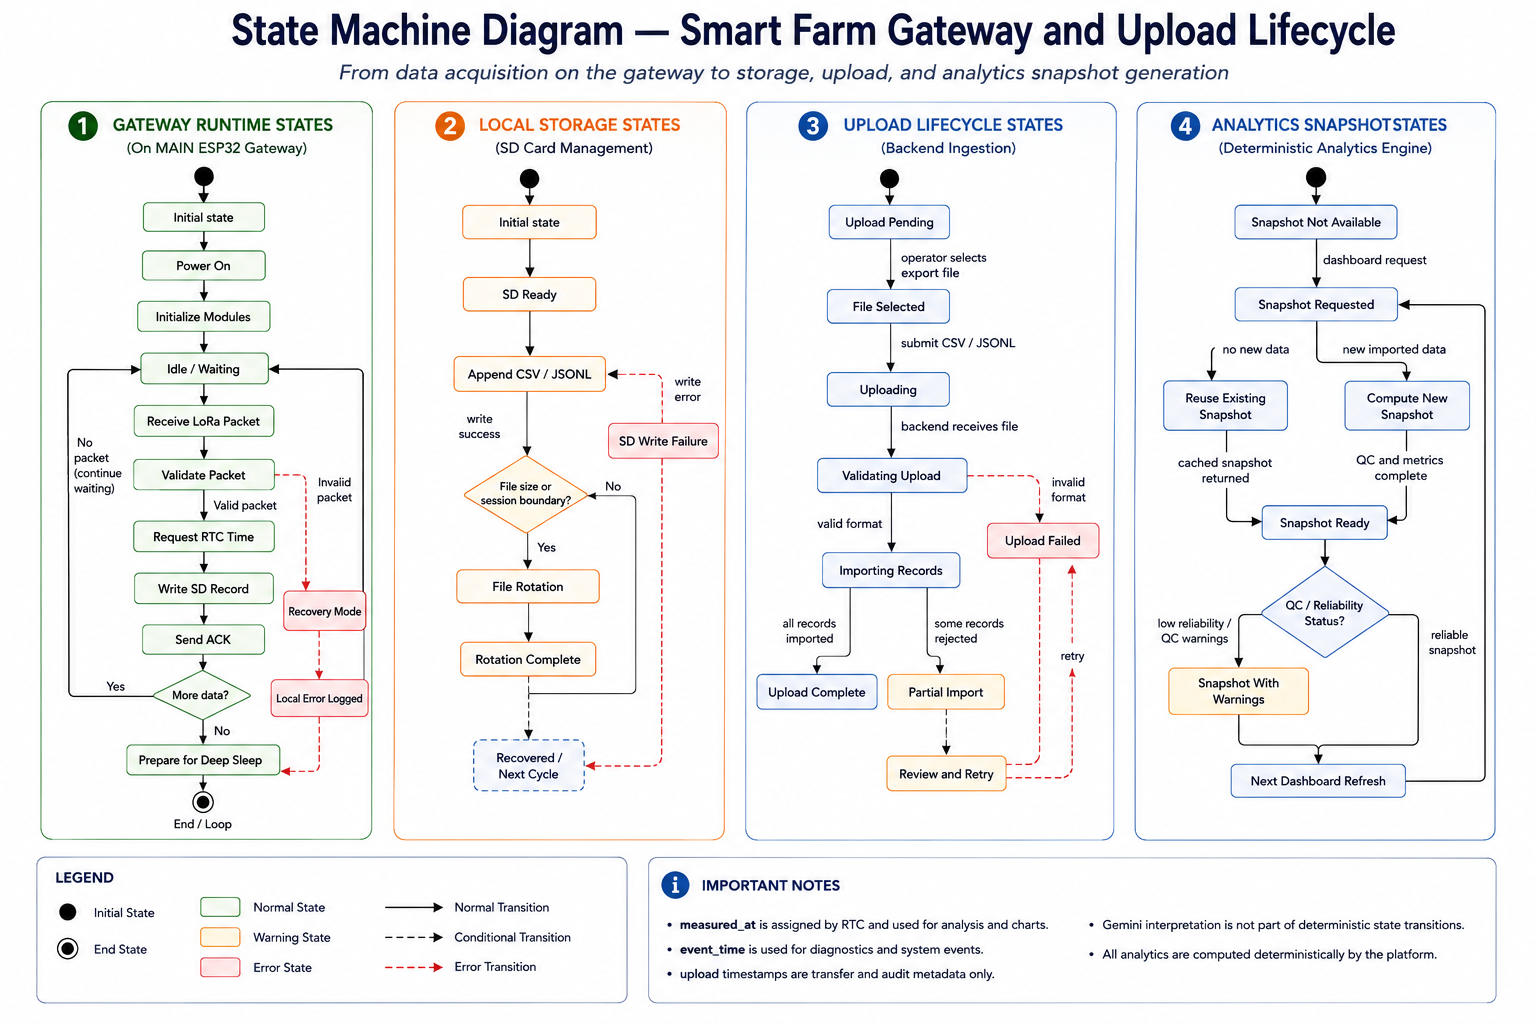
\includegraphics[width=0.85\textwidth]{figures/StateMachineDiagram}
% TODO: copy Academic-Thesis/Diagrams/State Machine Diagram.png to figures/StateMachineDiagram.png before compiling
\caption{Firmware state machine diagram showing the operating modes of the MAIN gateway node, their trigger conditions, and the transitions between them during normal operation, recovery, upload, and RTC synchronisation sequences.}
\label{fig:firmware-state-machine}
\end{figure}

% ----------------------------------------------------------
\subsection{Normal Sensing Mode}
\label{sec:mode-normal}
% ----------------------------------------------------------

Normal Sensing Mode is the default operating state, activated at the start of each ten-minute superframe. During this mode, the MAIN node opens its LoRa receive window to collect packets from Node2 and Node3, performs the Pivot~1 local soil reading, and writes all acquired data to the SD card before entering deep sleep.

The mode is not an always-on polling loop. Rather, it follows a scheduled sequence derived from the superframe timing. Node2 wakes at frame onset, powers its relay, performs its measurement, and transmits within the first 30~seconds of the frame. Node3 wakes independently and transmits shortly after. MAIN's receive window spans 70~seconds from frame start, providing sufficient margin to capture both remote transmissions before executing the local soil read. After SD writing, MAIN sleeps for the remainder of the ten-minute period.

% ----------------------------------------------------------
\subsection{Power Saving Mode}
\label{sec:mode-power-saving}
% ----------------------------------------------------------

Power Saving Mode was introduced in response to a fundamental constraint of the deployment environment: the three nodes are battery-powered, and the agricultural site does not provide stable mains electricity. Continuous sensor polling, continuous radio listening, and always-on sensor power would drain a battery within hours, rendering the system impractical.

The mode operates through four coordinated strategies. Deep sleep is the primary mechanism: the ESP32 and ESP32-C3 microcontrollers are placed in their lowest-power sleep state between measurement windows, with a timer interrupt as the sole wake source. Sensor power is controlled by the relay module; the relay is activated only for the warm-up and read interval and deactivated immediately after, preventing the RS485 soil sensor from drawing current between measurement cycles. The BME280 on Node3 is operated in forced mode, which similarly eliminates continuous sensor power draw. LoRa radio activity is confined to the transmission or reception window within each superframe; the transceiver is not listening or transmitting outside these windows.

Battery autonomy was not formally characterised during the validation window. The Power Saving Mode design is evaluated in qualitative terms: its constituent strategies reduce consumption during the idle intervals that constitute the majority of the ten-minute cycle.

% ----------------------------------------------------------
\subsection{LoRa RX/ACK Mode}
\label{sec:mode-lora-ack}
% ----------------------------------------------------------

During each superframe, the MAIN node operates its LoRa radio in receive mode for a window of 70~seconds. This window accommodates the expected transmission times of Node2 and Node3 with sufficient margin to absorb minor timing drift introduced by deep sleep wake-up jitter.

When a valid packet is received from a remote node, MAIN decodes and validates its contents, stamps the \texttt{measured\_at} field from the DS3231 RTC, writes the reading to the SD queue, and transmits an acknowledgement packet addressed to the source node. The ACK is not a bare confirmation; it carries the current RTC timestamp, which allows remote nodes to detect significant drift in their own sleep timers over extended operation.

The ACK mechanism serves two purposes. First, it confirms to the transmitting node that its packet was received correctly, which informs the node's reliability tracking and prevents redundant retransmission within the same cycle. Second, the ACK timestamp enables passive clock monitoring on remote nodes without requiring a dedicated synchronisation protocol. If a node does not receive an ACK within 1500~milliseconds of its transmission, it records a timeout and applies the Recovery Mode logic described in Section~\ref{sec:mode-recovery}.

% ----------------------------------------------------------
\subsection{Recovery Mode}
\label{sec:mode-recovery}
% ----------------------------------------------------------

Recovery Mode was motivated by a specific failure pattern observed during prototype testing: when a node failed to receive an ACK in one cycle — due to RF interference, timing misalignment, or transient hardware instability — it did not recover autonomously in the following cycle. Instead, the node's deep sleep counter drifted progressively further out of alignment with the MAIN receive window, causing repeated missed cycles until the node was manually power-cycled.

The failure mechanism is a timing mismatch, not merely a packet loss event. A node that sleeps 600~seconds expecting to wake into the MAIN receive window may wake slightly early or late; without ACK feedback, it cannot detect the drift and correct it. Over multiple cycles, small drift values accumulate until the node's transmission falls entirely outside the MAIN receive window.

Recovery Mode addresses this through two coordinated mechanisms. On the node side, an RTC\_DATA\_ATTR counter (\texttt{txFailCount}) persists across deep sleep cycles. Each consecutive ACK failure increments the counter. The node selects its next sleep duration from an adaptive sequence (60~seconds, 120~seconds, 300~seconds, 600~seconds) indexed by \texttt{txFailCount}. This sequence progressively shortens the sleep interval, causing the node to shift its transmission earlier in successive frames until it re-enters the MAIN receive window. On success (ACK received), \texttt{txFailCount} is reset to zero and normal sleep intervals resume.

On the MAIN side, a \texttt{NodeHealth} structure tracks each remote node's \texttt{missedCount} and \texttt{recoveryWatch} state. When a node is missed in a frame, MAIN extends its receive window from 70~seconds to 120~seconds for up to two consecutive frames. This extended window is designed to capture a recovering node whose transmission has shifted earlier than the standard window. If the node is not heard within the extended window over the tolerance period, MAIN logs a \texttt{node\_marked\_dead} event and returns to normal window timing. When the node reappears, a \texttt{node\_back\_online} event is logged and normal tracking resumes.

% ----------------------------------------------------------
\subsection{Local Storage Mode}
\label{sec:mode-storage}
% ----------------------------------------------------------

Local Storage Mode refers to the SD card write sequence that occurs at the end of each sensing cycle, after all LoRa receptions and the local soil read have completed. The MAIN node writes sensor readings to a CSV file and system events to a JSONL file. Both files accumulate across cycles, building an offline record of field conditions that persists independently of network availability.

\begin{figure}[H]
\centering
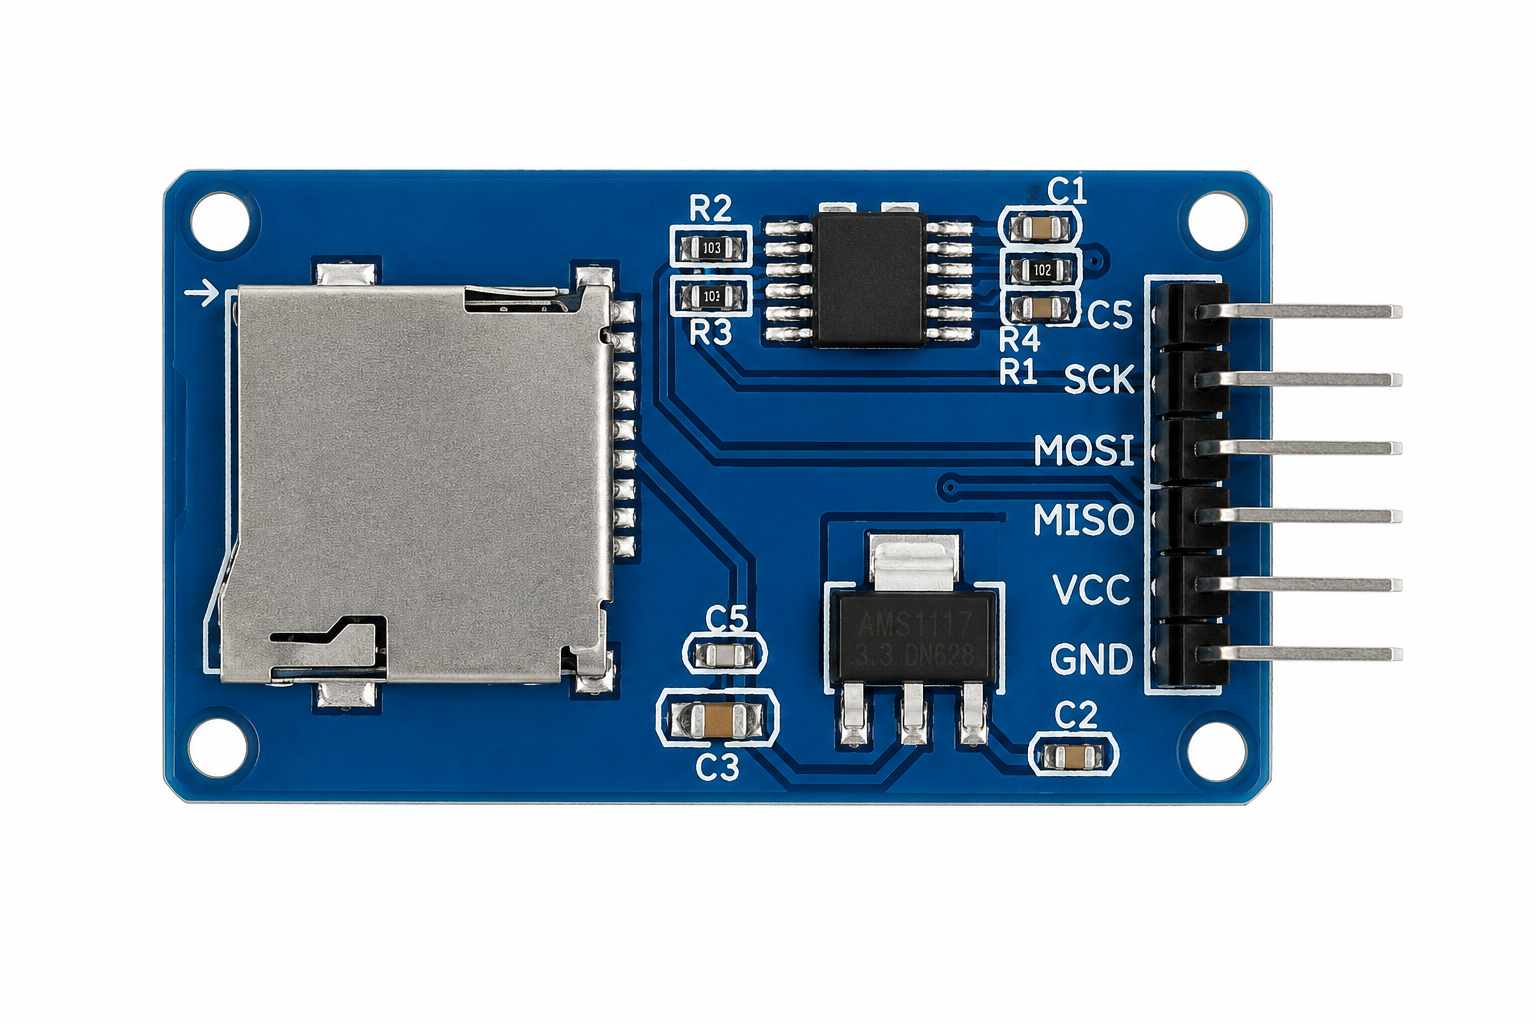
\includegraphics[width=0.30\textwidth]{figures/SdCardModule}
% TODO: copy Academic-Thesis/SystemImage/SdCardModule.png to figures/SdCardModule.png before compiling
\caption{SD card module mounted on the MAIN gateway node. The module uses the HSPI bus of the ESP32 and stores all sensor readings and system events in CSV and JSONL format, providing offline persistence between upload sessions.}
\label{fig:sd-card-module}
\end{figure}

The CSV format is used for sensor readings because it supports efficient append operations and is directly portable to analytics tools. JSONL is used for system events because each event carries a variable-length JSON object with fields that differ by event type. The SD card is the only storage mechanism; no data is held in ESP32 flash between cycles, as the deep sleep state clears RAM. Data acquisition continues uninterrupted across days or weeks without Internet access; the SD card accumulates the full measurement history until Upload Mode is manually triggered.

% ----------------------------------------------------------
\subsection{Upload Mode}
\label{sec:mode-upload}
% ----------------------------------------------------------

Upload Mode is triggered by a sustained press of the GPIO34 button on the MAIN node, requiring contact of at least one second. The sustained trigger distinguishes Upload Mode from the four-consecutive-press sequence used for RTC synchronisation and from brief accidental contact.

The mode was designed around the reality of intermittent Internet access in Saharan field environments. Continuous upload would require a persistent mobile data connection, which is neither cost-effective nor reliable at agricultural field sites. The offline-first design accumulates data locally and transfers it in a single batch when connectivity becomes temporarily available.

During Upload Mode, MAIN reads the accumulated CSV and JSONL files from the SD card and transmits their contents to the WebService backend via the POST \texttt{/api/v1/upload} endpoint. The backend processes each record by inserting sensor readings into the \texttt{sensor\_readings} table using the \texttt{measured\_at} timestamp from the SD record, and system events into the \texttt{system\_events} table using the \texttt{event\_time} field. The upload transaction's own timestamp is stored in the \texttt{uploads} table as transfer metadata. This timestamp serves as an audit record of when data was transmitted; it is not used in any analytical query, chart, or dashboard computation. The distinction is enforced in the backend ingestion logic and documented in the data-field policy described in Section~\ref{sec:storage-time}.

% ----------------------------------------------------------
\subsection{RTC Synchronisation Mode}
\label{sec:mode-rtc-sync}
% ----------------------------------------------------------

RTC Synchronisation Mode corrects the DS3231 real-time clock when the stored time has drifted or when the battery was replaced. Measurement timestamps are derived exclusively from the DS3231; any persistent drift would introduce systematic errors in the \texttt{measured\_at} values for all readings acquired before the correction.

\begin{figure}[H]
\centering
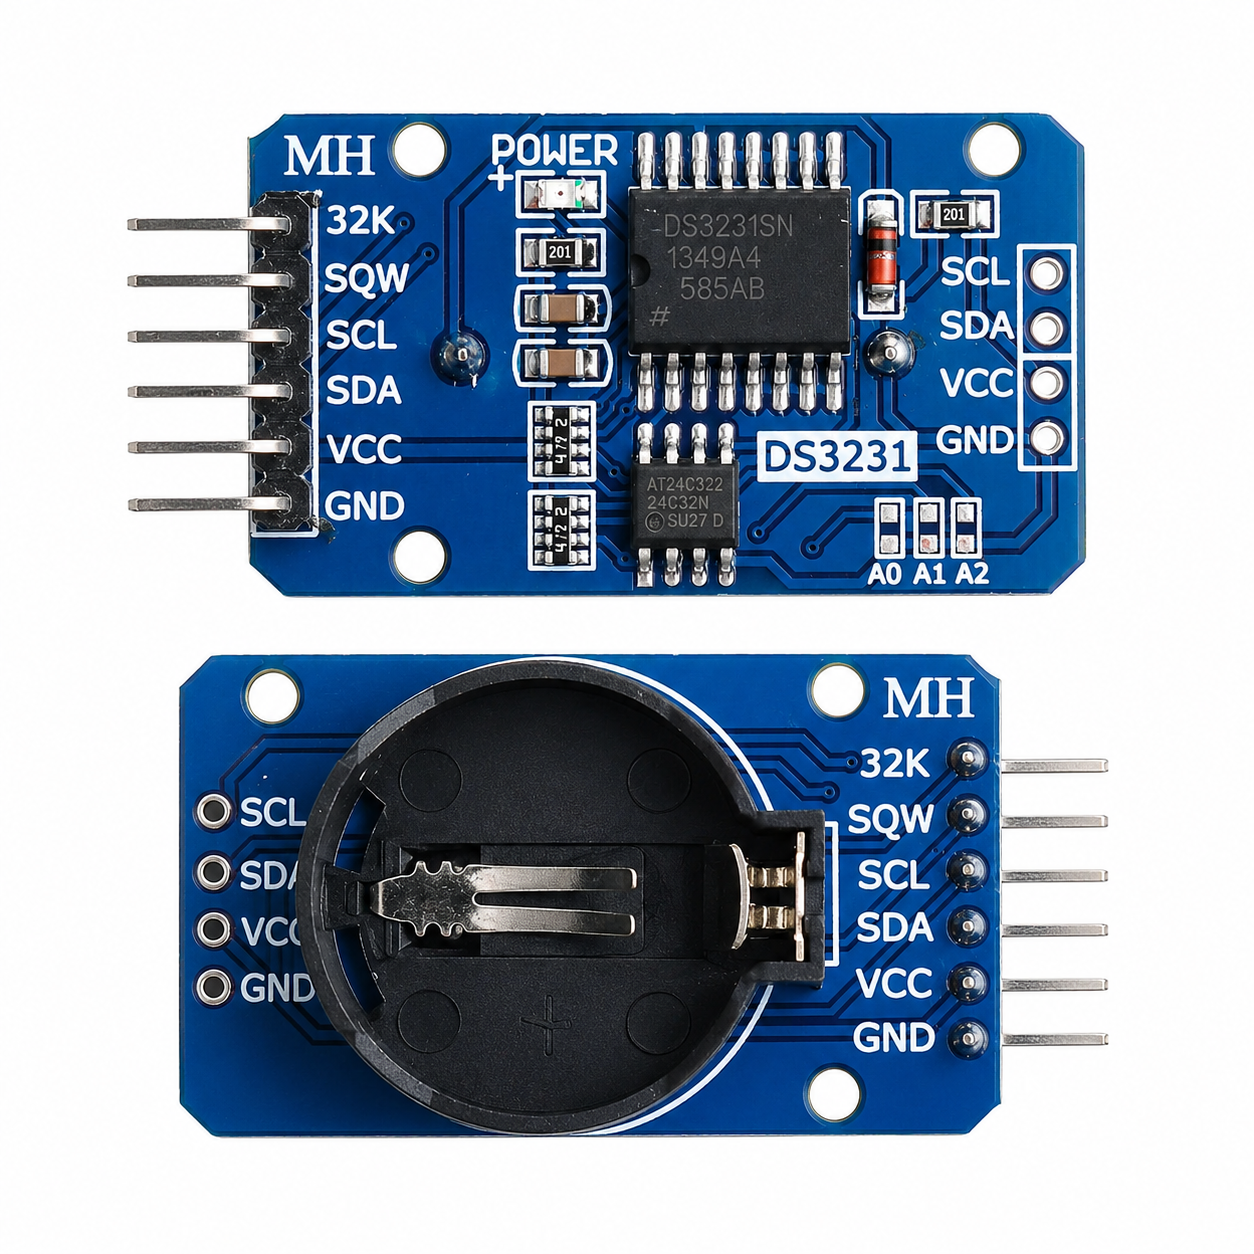
\includegraphics[width=0.30\textwidth]{figures/Rtc}
% TODO: copy Academic-Thesis/SystemImage/Rtc.png to figures/Rtc.png before compiling
\caption{DS3231 RTC module mounted on the MAIN gateway node. The module provides battery-backed timekeeping and is the exclusive source of \texttt{measured\_at} timestamps for all sensor readings.}
\label{fig:rtc-module}
\end{figure}

The mode is triggered by four consecutive short presses of the GPIO34 button. MAIN initiates a connection to the WebService backend and sends a synchronisation request. The backend responds with the current server time in the \texttt{server\_time} field of the JSON response. MAIN parses this value and writes it to the DS3231 over I2C. All subsequent readings are timestamped from the updated clock. The synchronisation event is logged to the SD card and transmitted to the backend as a system event, providing an audit record of when the RTC was last corrected.

% ----------------------------------------------------------
\subsection{Diagnostic Logging Mode}
\label{sec:mode-diagnostic}
% ----------------------------------------------------------

Diagnostic Logging Mode is not a separate operating state but a cross-cutting concern active throughout all other modes. Whenever a noteworthy event occurs — a failed ACK, a node entering recovery, a successful recovery, a node marked as no longer communicating, an SD write error, a sensor read failure, or an upload transaction — the MAIN node writes a structured record to the JSONL event file on the SD card.

These event records carry a type field (for example: \texttt{recovery\_started}, \texttt{recovery\_cycle\_adjusted}, \texttt{recovery\_success}, \texttt{recovery\_failed}, \texttt{node\_marked\_dead}, \texttt{node\_back\_online}), a \texttt{event\_time} derived from the DS3231, and a payload containing mode-specific context. During upload, the event records are transmitted to the backend alongside sensor readings and stored in the \texttt{system\_events} table. The dashboard's diagnostics view draws from this table to present a timeline of system health events to the operator.

The logging mechanism serves a dual purpose. During field testing, it enabled the diagnosis of the timing-drift failure that motivated Recovery Mode. In production use, it provides the operator with evidence to distinguish sensor malfunction, communication outage, and firmware-level issues without physical access to the node.

\bigskip

Table~\ref{tab:firmware-operating-modes} consolidates the eight firmware modes with their trigger conditions, field motivations, and outputs.

\begin{table}[H]
\centering
\caption{Firmware operating modes of the proposed system, showing trigger conditions, motivations, and outputs.}
\label{tab:firmware-operating-modes}
\small
\begin{tabular}{p{2.5cm} p{2.8cm} p{3.0cm} p{3.2cm} p{2.5cm}}
\hline
\textbf{Mode} & \textbf{Trigger} & \textbf{Purpose} & \textbf{Field problem addressed} & \textbf{Output / log} \\
\hline
Normal Sensing & Superframe timer wake & Scheduled sensor acquisition and SD storage & Periodic monitoring without continuous power & CSV reading row; SD write \\
\hline
Power Saving & Always active between cycles & Deep sleep, relay power control, BME280 forced mode & Battery longevity in off-grid deployment & Reduced active duty cycle \\
\hline
LoRa RX/ACK & MAIN receive window open & Receive remote node packets; send ACK with RTC time & Loss of remote data without confirmation feedback & SD write; ACK packet; \texttt{node\_back\_online} event \\
\hline
Recovery & ACK failure increments \texttt{txFailCount} & Adaptive sleep adjustment to re-enter MAIN window & Timing drift causing persistent missed cycles & JSONL event: \texttt{recovery\_started}, \texttt{recovery\_cycle\_adjusted}, \texttt{recovery\_success}, \texttt{recovery\_failed} \\
\hline
Local Storage & End of each sensing cycle & Persist readings and events to SD & Data loss during Internet-unavailable periods & CSV row appended; JSONL event appended \\
\hline
Upload & Long button press ($\geq$1~s) & Batch transfer of SD content to backend & Continuous upload impractical at field site & POST to \texttt{/api/v1/upload}; \texttt{uploads} table row; upload JSONL event \\
\hline
RTC Synchronisation & Four consecutive button presses & Correct DS3231 clock drift; server time written & Drift in measurement timestamps over weeks & RTC updated; sync event logged \\
\hline
Diagnostic Logging & Continuous (all modes) & Record system health events with timestamps & No remote visibility into node/gateway health & JSONL event file; \texttt{system\_events} table row \\
\hline
\end{tabular}
\end{table}

% ============================================================
\section{Communication Design}
\label{sec:ch3-communication}
% ============================================================

All wireless communication in the system uses LoRa, a spread-spectrum modulation technique operating at 433~MHz in the ISM band. The physical layer parameters are configured identically on all three nodes to ensure mutual decoding: spreading factor SF7, bandwidth 125~kHz, coding rate 4/5, CRC enabled, and transmit power 14~dBm. SF7 was chosen to balance airtime, energy per packet, and link budget for the distances anticipated between nodes and the MAIN gateway in the target agricultural field. The justification for the LoRa selection was established in Section~\ref{sec:communication}.

\begin{figure}[H]
\centering
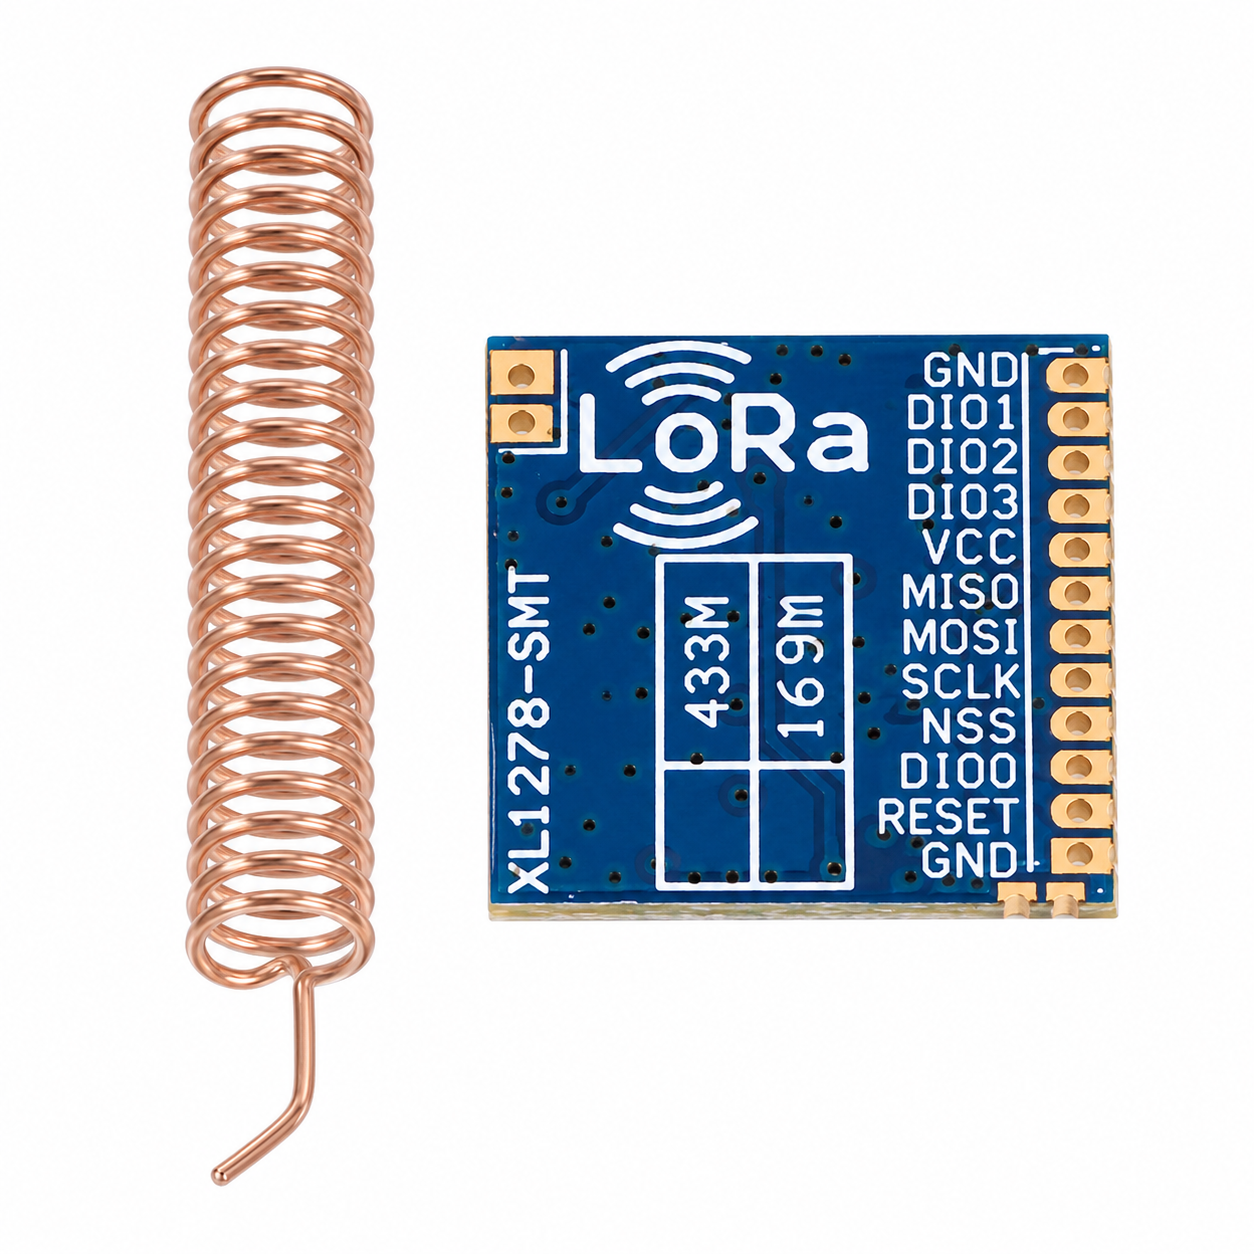
\includegraphics[width=0.35\textwidth]{figures/LoRa}
% TODO: copy Academic-Thesis/SystemImage/LoRa.png to figures/LoRa.png before compiling
\caption{SX127x LoRa transceiver module used on all three nodes. The module operates at 433~MHz and is configured with identical parameters across the system to ensure compatibility between the transmitting remote nodes and the receiving MAIN gateway.}
\label{fig:lora-module-ch3}
\end{figure}

Communication follows a structured superframe pattern rather than contention-based access. Node2 transmits first, at approximately 24~seconds into the ten-minute frame. Node3 transmits at approximately 38~seconds. MAIN's receive window spans the first 70~seconds of the frame, providing margin for each node. Because only one node transmits during each sub-window, collision risk is minimal under normal operation.

\begin{figure}[H]
\centering
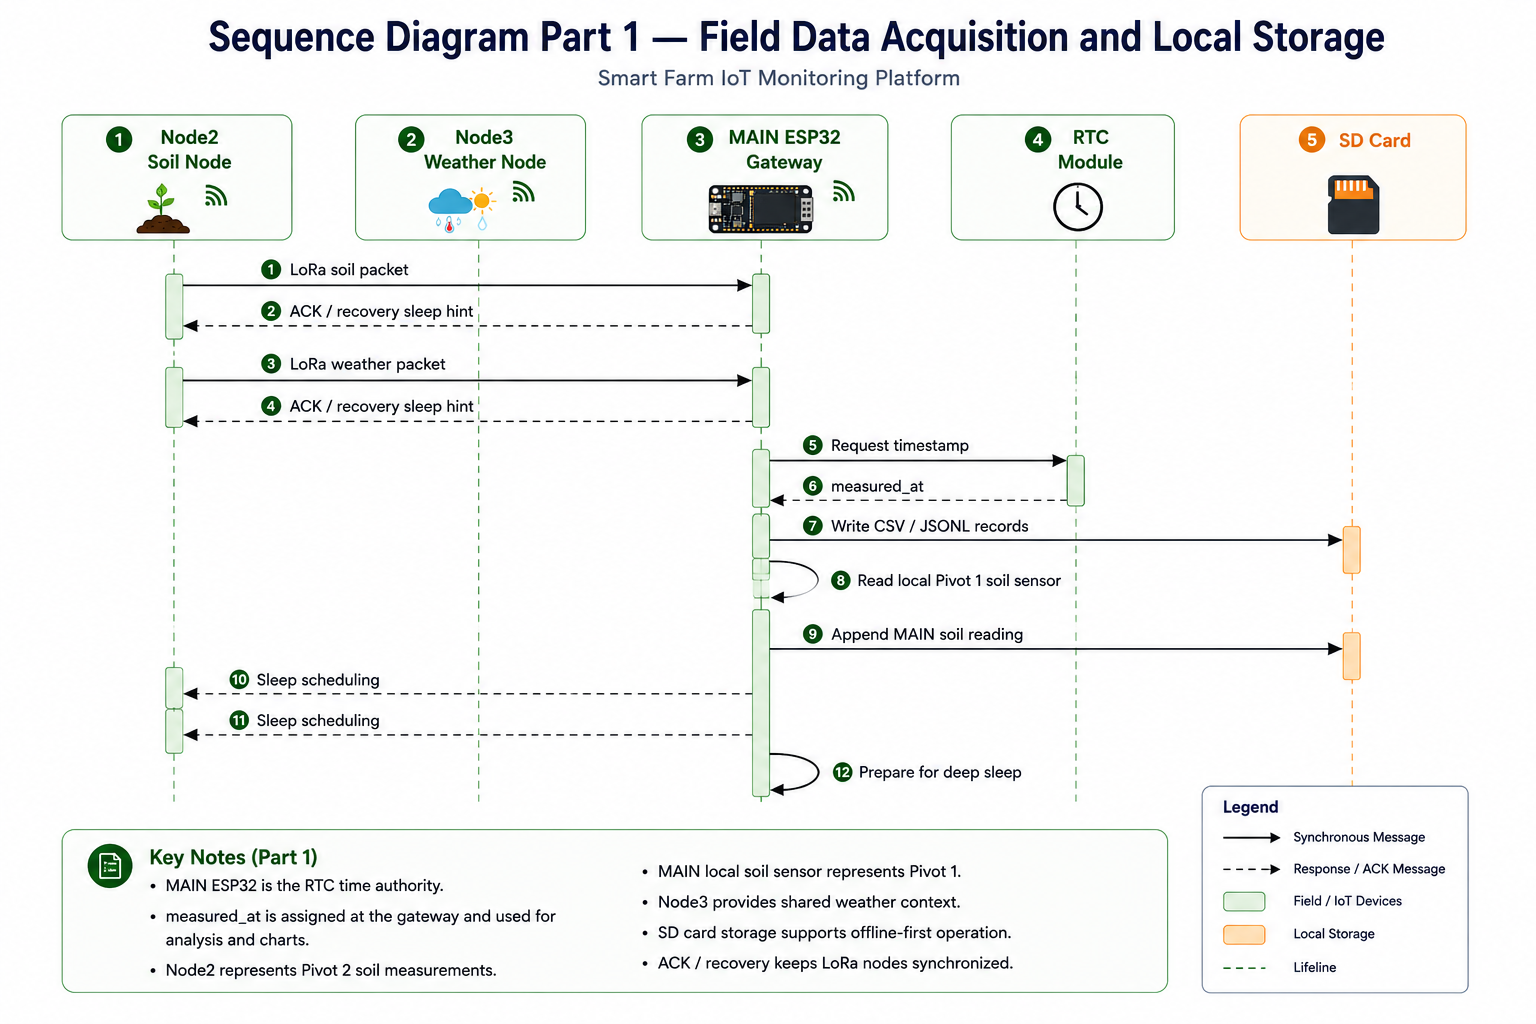
\includegraphics[width=\textwidth]{figures/SequenceDiagram1}
% TODO: confirm whether Academic-Thesis/Diagrams/Sequence Diagrams.png is one file or two separate files (Sequence Diagrams 1.png and Sequence Diagrams 2.png); copy the appropriate file(s) to figures/SequenceDiagram1.png before compiling
\caption{Sequence diagram illustrating the LoRa communication flow during a normal sensing cycle, showing Node2 and Node3 transmissions, MAIN reception and acknowledgement, local soil read, and SD storage sequence.}
\label{fig:sequence-diagram-1}
\end{figure}

\begin{figure}[H]
\centering
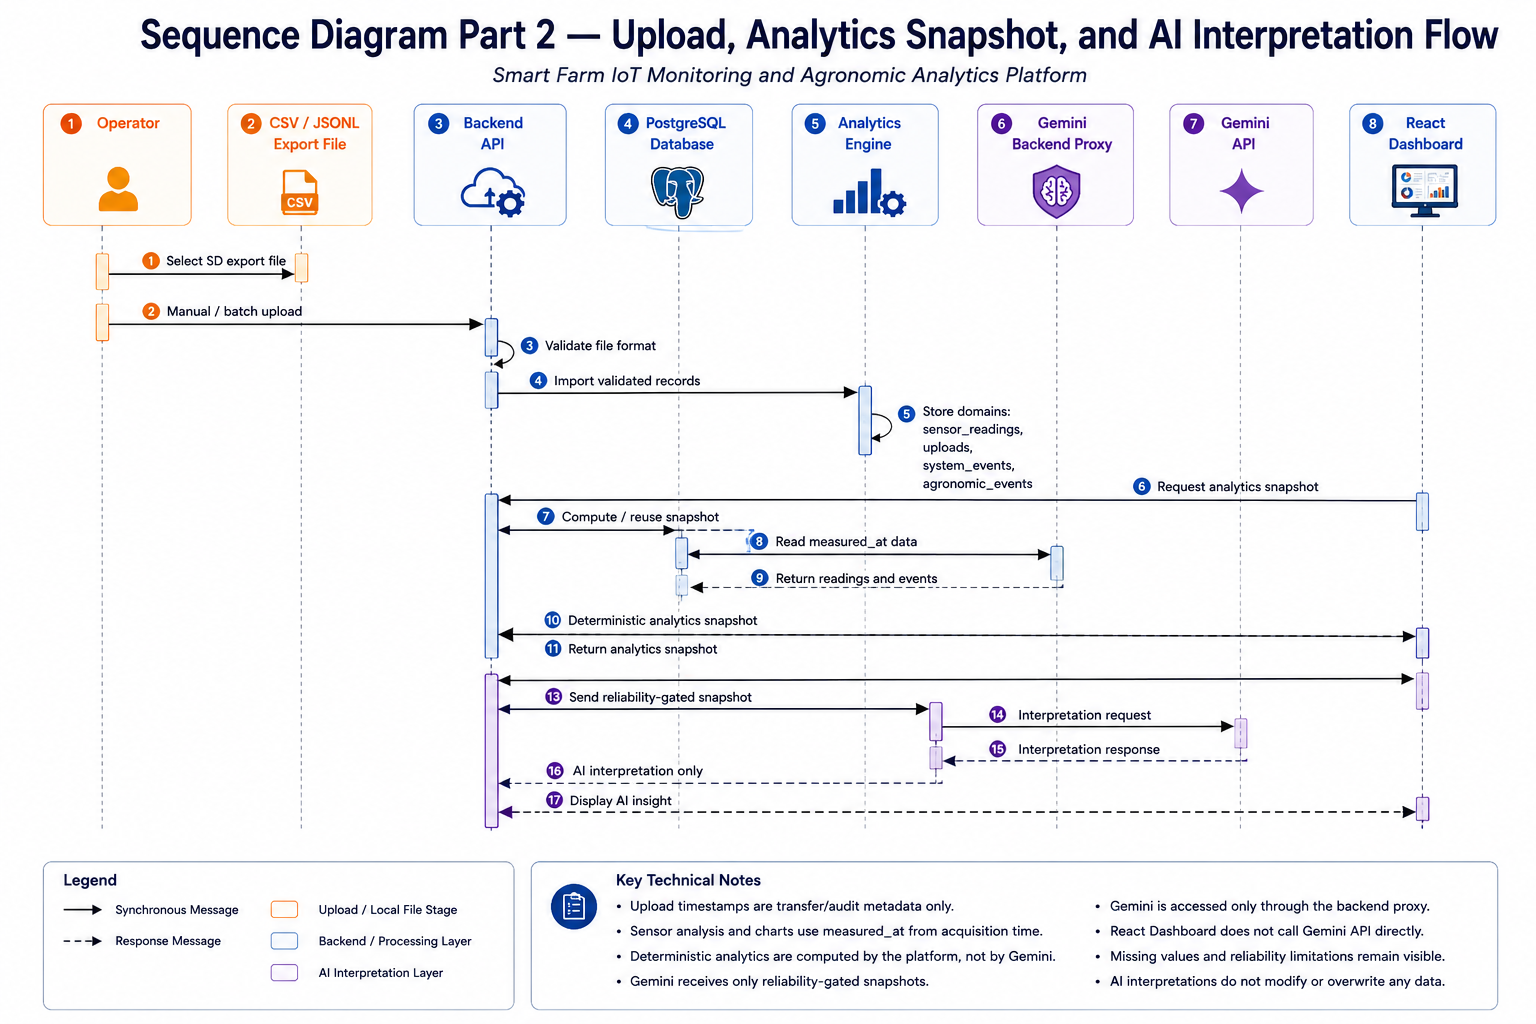
\includegraphics[width=\textwidth]{figures/SequenceDiagram2}
% TODO: confirm whether a second sequence diagram file exists for the recovery and upload flows; copy to figures/SequenceDiagram2.png if confirmed; otherwise remove this figure and its reference
\caption{Sequence diagram illustrating the communication sequence during Recovery Mode, showing the adaptive retry mechanism when a remote node fails to receive an ACK, and the eventual re-synchronisation with the MAIN receive window.}
\label{fig:sequence-diagram-2}
\end{figure}

Each LoRa packet carries a structured payload. The payload includes a node identifier, the sensor measurement values (three integers from the Modbus register map for soil nodes; three floats from the BME280 for the weather node), a firmware stage constant indicating the node's progress through the superframe, and a CRC byte for payload integrity. MAIN decodes the node identifier, validates the CRC, and stamps the packet with \texttt{measured\_at} from the DS3231 before writing the reading to SD.

The ACK packet is transmitted by MAIN within the receive window immediately after a successful packet decode. It carries the current RTC timestamp and an echo of the source node identifier. If a node does not receive the ACK within 1500~milliseconds of its own transmission, it registers a miss and the Recovery Mode logic described in Section~\ref{sec:mode-recovery} applies on the next cycle.

The RSSI values recorded in the validation dataset (spanning the range from approximately $-76$~dBm to $-97$~dBm across the observation window) confirm that functional communication was maintained between the nodes and the MAIN gateway throughout the validation period. Formal range characterisation over measured distances was not conducted; the system is not described in terms of a guaranteed communication range.

% ============================================================
\section{Data Storage and Time Policy}
\label{sec:storage-time}
% ============================================================

The data model of the system is organised into four canonical domains, each with a distinct time field that reflects the semantic role of the domain. The policy governing these fields is enforced at every layer of the implementation, from firmware SD writes through backend ingestion to dashboard queries.

The central principle of the time policy is that the time of measurement and the time of upload are distinct and must never be conflated. This distinction was identified in Chapter~\ref{chap:related-works} as a gap in several reviewed systems, where upload timestamps were used as proxies for measurement time in stored records and dashboard charts. In the proposed system, the \texttt{measured\_at} field is written by the MAIN gateway firmware from the DS3231 RTC at the moment a packet is received and validated; it is not modifiable by subsequent processing steps. The \texttt{uploaded\_at} field in the \texttt{uploads} table records when the SD batch was transmitted to the backend; it is stored as transfer audit metadata and is not referenced in any analytical query, chart computation, or dashboard visualisation.

\begin{table}[H]
\centering
\caption{Data domains, primary time fields, and analytical roles in the proposed storage model.}
\label{tab:data-domains-time-fields}
\small
\begin{tabular}{p{3.0cm} p{4.0cm} p{2.8cm} p{1.5cm} p{3.0cm}}
\hline
\textbf{Data domain} & \textbf{Stored content} & \textbf{Primary time field} & \textbf{Used for analytics?} & \textbf{Purpose} \\
\hline
\texttt{sensor\_readings} & Soil moisture, soil temperature, soil EC, air temperature, air humidity, barometric pressure & \texttt{measured\_at} (DS3231 RTC) & Yes & Trend charts, quality checking, reliability scoring, threshold alerts \\
\hline
\texttt{system\_events} & Recovery events, upload events, node status changes, sensor errors, SD errors & \texttt{event\_time} (DS3231 RTC) & Yes (diagnostics only) & System health timeline; diagnostics dashboard panel \\
\hline
\texttt{uploads} & Upload transaction metadata; SD batch reference; record counts & \texttt{uploaded\_at} (server time of receipt) & No — transfer audit metadata only & Audit trail of when SD batches were transmitted; never used as measurement time \\
\hline
\texttt{agronomic\_events} & Irrigation sessions, harvest events, fertilisation records, operator notes & \texttt{started\_at} / \texttt{ended\_at} (operator-entered) & Yes (agronomic context layer) & Contextual overlay on measurement charts; agronomic timeline \\
\hline
\end{tabular}
\end{table}

The upload timestamp is transfer and audit metadata only. It is recorded to provide a traceable log of when each SD batch was received by the backend, supporting diagnosis of upload failures and data completeness checks. It does not appear on any measurement chart axis, is not used in any filtering or aggregation query on sensor readings, and is never presented to the operator as an approximation of when a measurement was taken. This separation is not merely a policy declaration; it is enforced structurally in the backend ingestion logic: the upload endpoint inserts each reading using the \texttt{measured\_at} value from the SD record, and the upload transaction's own timestamp is stored exclusively in the \texttt{uploads} table, which is not joined to the \texttt{sensor\_readings} table in any analytical query.

All timestamps are stored in UTC at the database level. The dashboard converts UTC values to Algeria Standard Time (UTC+1) for display, as documented in the backend configuration. Agronomic event times are entered by the operator through the dashboard interface; they are stored in the \texttt{agronomic\_events} table with separate \texttt{started\_at} and \texttt{ended\_at} fields to support duration-based queries and chart overlay rendering.

% ============================================================
\section{Backend Implementation}
\label{sec:backend}
% ============================================================

The backend is implemented as a Node.js application using the Express.js framework, connected to a PostgreSQL relational database. It exposes a REST API secured by an API key, consumed by both the MAIN gateway firmware during Upload Mode and the React web dashboard for data retrieval and display.

The backend serves three categories of client requests. The firmware upload client issues POST requests to transmit SD batch content after each Upload Mode session. The dashboard client issues GET requests to retrieve readings, events, analytics snapshots, and agronomic events for display. Administrative clients may issue POST requests to create or update agronomic events through the dashboard interface.

\begin{figure}[H]
\centering
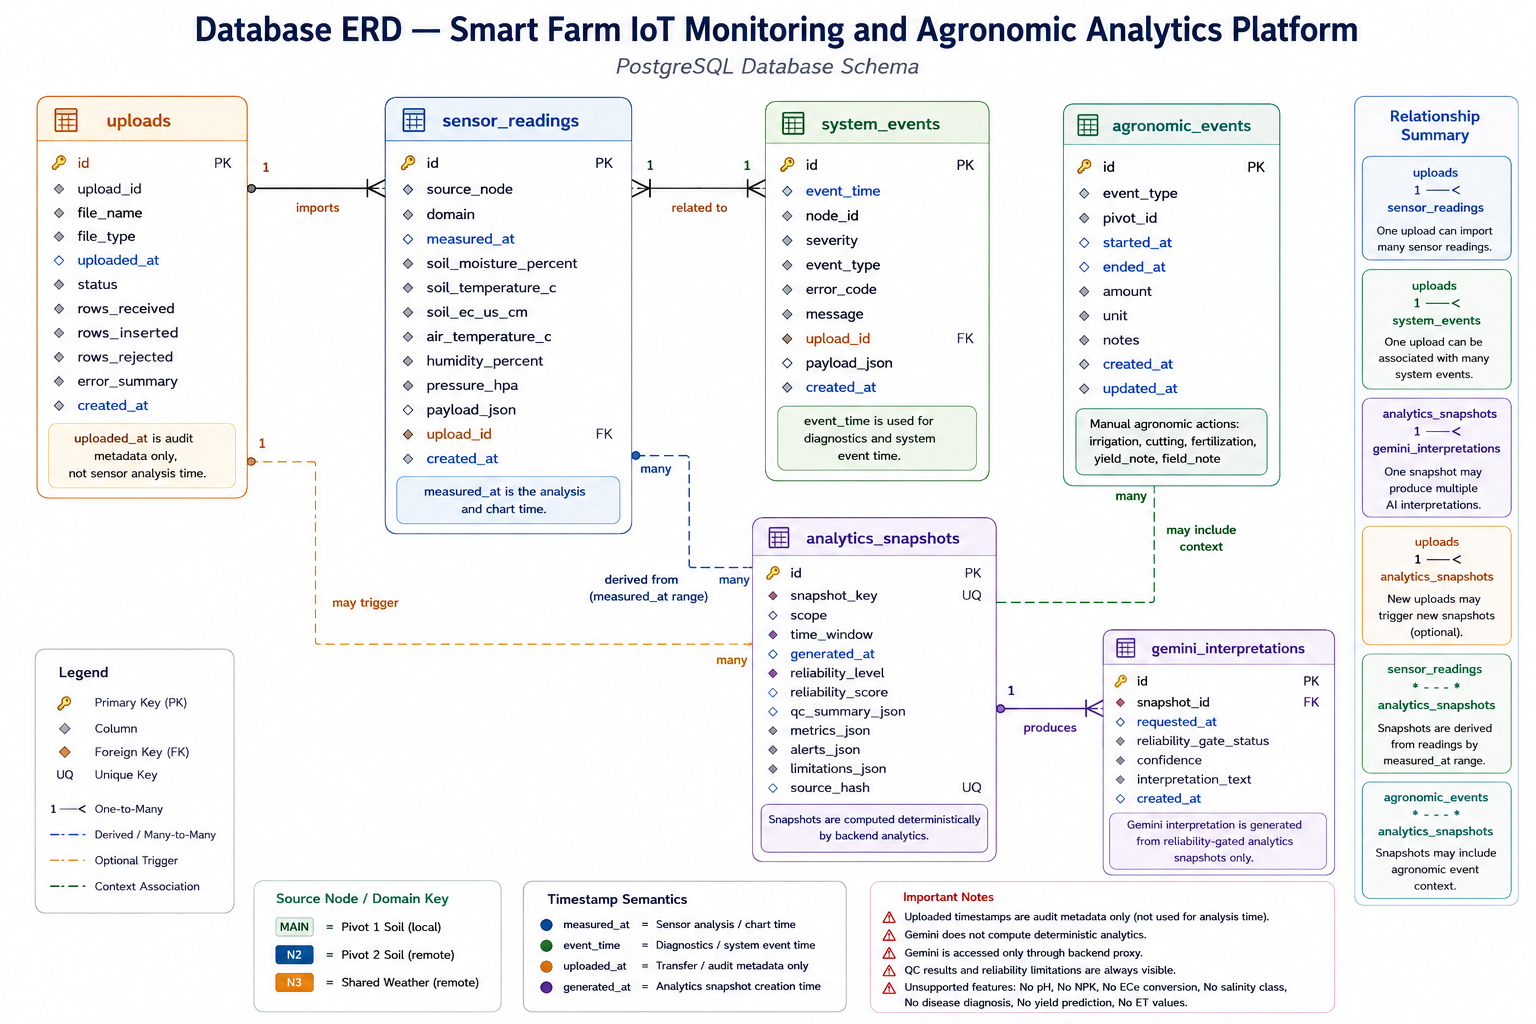
\includegraphics[width=\textwidth]{figures/DatabaseERDDiagram}
% TODO: copy Academic-Thesis/Diagrams/DatabaseERDDiagram.png to figures/DatabaseERDDiagram.png before compiling
\caption{Entity-relationship diagram of the PostgreSQL database, showing the \texttt{gateways}, \texttt{nodes}, \texttt{sensor\_readings}, \texttt{system\_events}, \texttt{uploads}, \texttt{agronomic\_events}, and \texttt{analytics\_snapshots} tables and their relationships.}
\label{fig:database-erd}
\end{figure}

The database schema is organised in four SQL migration files. The initial migration (\texttt{001\_init.sql}) creates the \texttt{gateways}, \texttt{nodes}, \texttt{sensor\_readings}, \texttt{system\_events}, and \texttt{uploads} tables. A patch migration (\texttt{002\_patch.sql}) applies corrections to column definitions. The agronomic migration (\texttt{003\_agronomic.sql}) adds the \texttt{agronomic\_events} table. The analytics migration (\texttt{004\_analytics\_snapshots.sql}) adds the \texttt{analytics\_snapshots} table, which stores the output of the deterministic analytics pipeline described in Part~B. Table~\ref{tab:database-tables} summarises the implemented tables and their roles.

\begin{table}[H]
\centering
\caption{PostgreSQL database tables implemented in the WebService backend.}
\label{tab:database-tables}
\small
\begin{tabular}{p{3.8cm} p{2.5cm} p{7.0cm}}
\hline
\textbf{Table} & \textbf{Migration} & \textbf{Purpose and key fields} \\
\hline
\texttt{gateways} & 001\_init & Registered MAIN gateway devices; gateway identifier, name, API key hash \\
\hline
\texttt{nodes} & 001\_init & Registered remote nodes; node identifier, gateway reference, node type \\
\hline
\texttt{sensor\_readings} & 001\_init & All sensor measurements; \texttt{measured\_at} (RTC-derived), soil and weather values, node reference \\
\hline
\texttt{system\_events} & 001\_init & Firmware diagnostic events; \texttt{event\_time} (RTC-derived), event type, payload \\
\hline
\texttt{uploads} & 001\_init & Upload transaction records; \texttt{uploaded\_at} (server receipt time), record counts, gateway reference; transfer audit metadata only \\
\hline
\texttt{agronomic\_events} & 003\_agronomic & Operator-recorded field events; \texttt{started\_at}, \texttt{ended\_at}, event type, notes \\
\hline
\texttt{analytics\_snapshots} & 004\_analytics & Output of deterministic analytics pipeline; snapshot timestamp, quality scores, reliability indicator, alert flags \\
\hline
\end{tabular}
\end{table}

The upload ingestion process follows a defined sequence. The firmware transmits a JSON body containing arrays of sensor reading objects and system event objects, each carrying the time fields written by the firmware to SD. The backend validates the API key, creates an \texttt{uploads} record with the server receipt timestamp, then iterates over each reading object and inserts a row into \texttt{sensor\_readings} using the \texttt{measured\_at} value from the firmware-provided object. System events are inserted into \texttt{system\_events} using the \texttt{event\_time} value from the firmware-provided object. At no point does the backend substitute the upload receipt timestamp for any measurement-derived time field.

\begin{table}[H]
\centering
\caption{Backend REST API endpoints and their functions.}
\label{tab:api-endpoints}
\small
\begin{tabular}{p{1.5cm} p{4.5cm} p{2.5cm} p{5.0cm}}
\hline
\textbf{Method} & \textbf{Endpoint} & \textbf{Client} & \textbf{Function} \\
\hline
POST & \texttt{/api/v1/upload} & Firmware (Upload Mode) & Ingest SD batch; insert readings, events, uploads; return server time for optional RTC sync \\
\hline
GET & \texttt{/api/v1/readings} & Dashboard & Retrieve sensor readings filtered by node, time range, and measurement domain \\
\hline
GET & \texttt{/api/v1/events} & Dashboard & Retrieve system events for diagnostics timeline \\
\hline
GET & \texttt{/api/v1/agronomic-events} & Dashboard & Retrieve agronomic events for chart overlay and event log \\
\hline
POST & \texttt{/api/v1/agronomic-events} & Dashboard & Create a new agronomic event record \\
\hline
GET & \texttt{/api/v1/analytics} & Dashboard & Retrieve analytics snapshots for the Processed Data Viewer \\
\hline
POST & \texttt{/api/v1/gemini} & Dashboard & Forward deterministic snapshot to Gemini and return narrative response; AI boundary enforced \\
\hline
\end{tabular}
\end{table}

% TODO: add captured API response samples if available — see missing_items H5

The \texttt{/api/v1/gemini} endpoint enforces the AI interpretation boundary described in the system requirements. The endpoint receives the deterministic analytics snapshot computed by the backend pipeline, not raw sensor readings, and forwards it to the Gemini model via the Google AI API. The model is not given access to the raw database, is not asked to compute statistics, and is not instructed to produce agronomic prescriptions. The response is returned to the dashboard and presented to the operator under a label that identifies it as an AI-generated interpretive narrative. The analytical layer — quality scores, reliability indicator, and threshold alerts — is computed entirely by the deterministic pipeline and is not modified by the AI response.

% ============================================================
\section{Dashboard Implementation}
\label{sec:dashboard}
% ============================================================

The web dashboard is implemented as a React application built with the Vite toolchain and TypeScript. It serves as the visualization and monitoring layer of the system, presenting uploaded and processed data to the operator through a set of purpose-built interface pages. The dashboard does not establish a persistent sensor connection or stream data in real time; it reflects the state of the backend database at the point of the most recent upload session. This design follows from the offline-first architecture described in Section~\ref{sec:storage-time}: connectivity is intermittent, and the authoritative measurement record resides on the SD card until an upload session transfers it to the backend.

\begin{figure}[H]
\centering
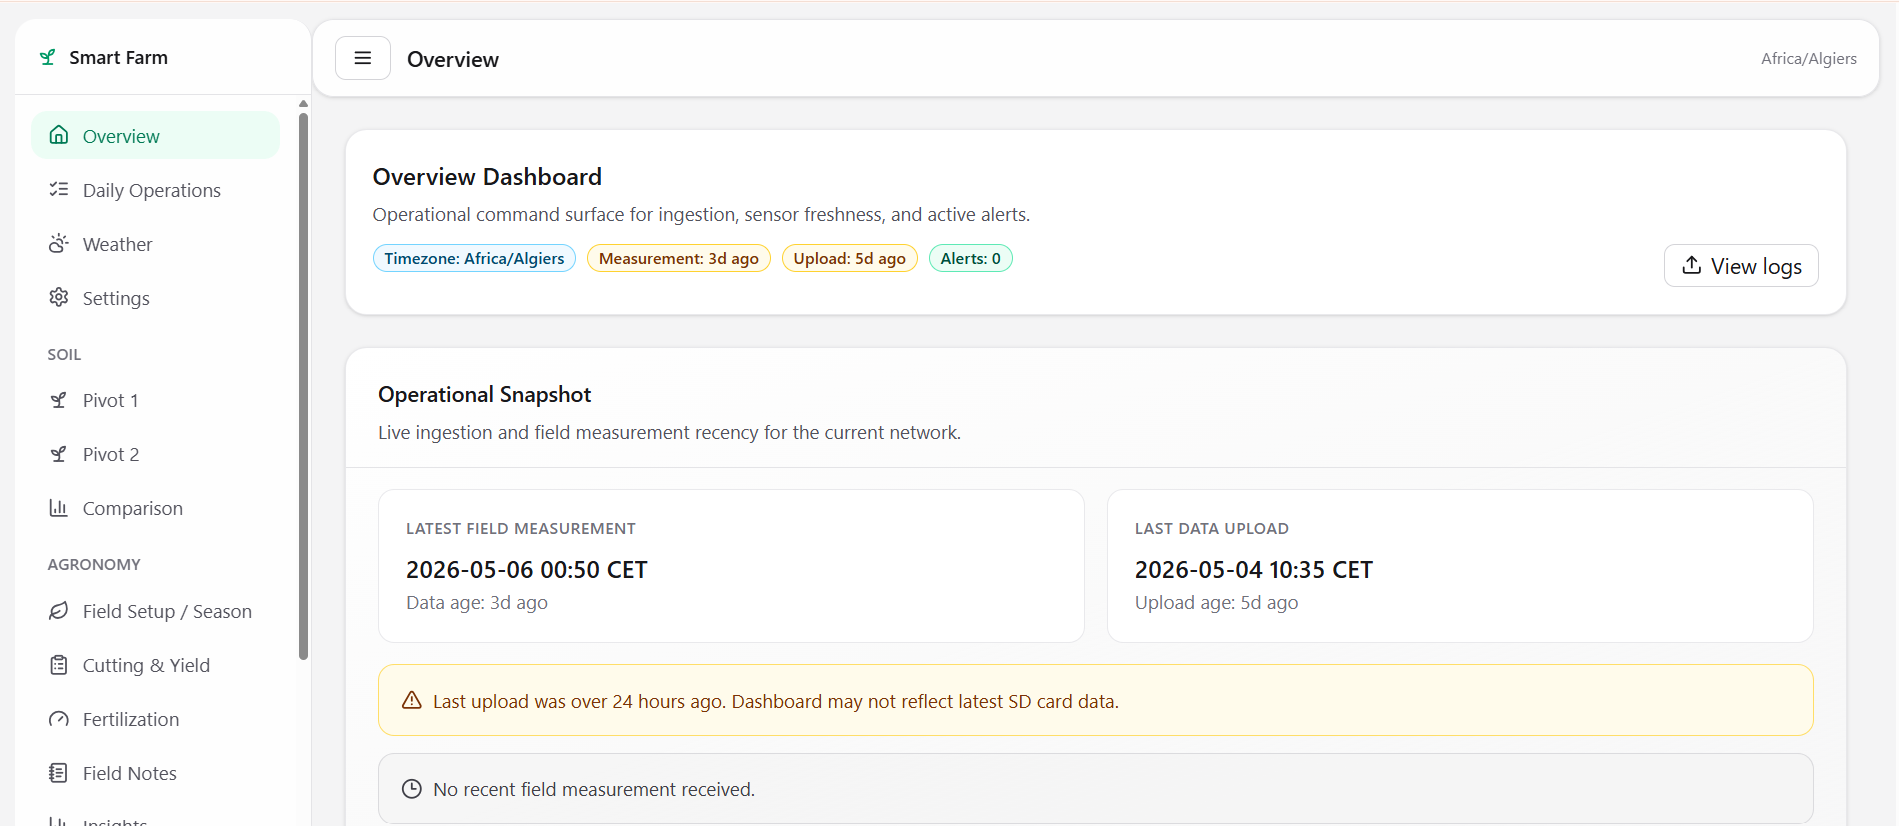
\includegraphics[width=\textwidth]{figures/DashOverview}
% TODO: copy Academic-Thesis/DashBoredImages/Overview.png to figures/DashOverview.png before compiling
\caption{Dashboard overview page presenting a summary of the latest uploaded sensor readings, system status, and navigation to domain-specific pages.}
\label{fig:dashboard-overview}
\end{figure}

The overview page provides a consolidated summary of the latest sensor values received from the three nodes, alongside navigation to domain-specific pages. It does not display a live sensor feed; instead, it reflects the most recently ingested batch, allowing the operator to confirm that the last upload session was successful before proceeding to detailed analysis.

\begin{figure}[H]
\centering
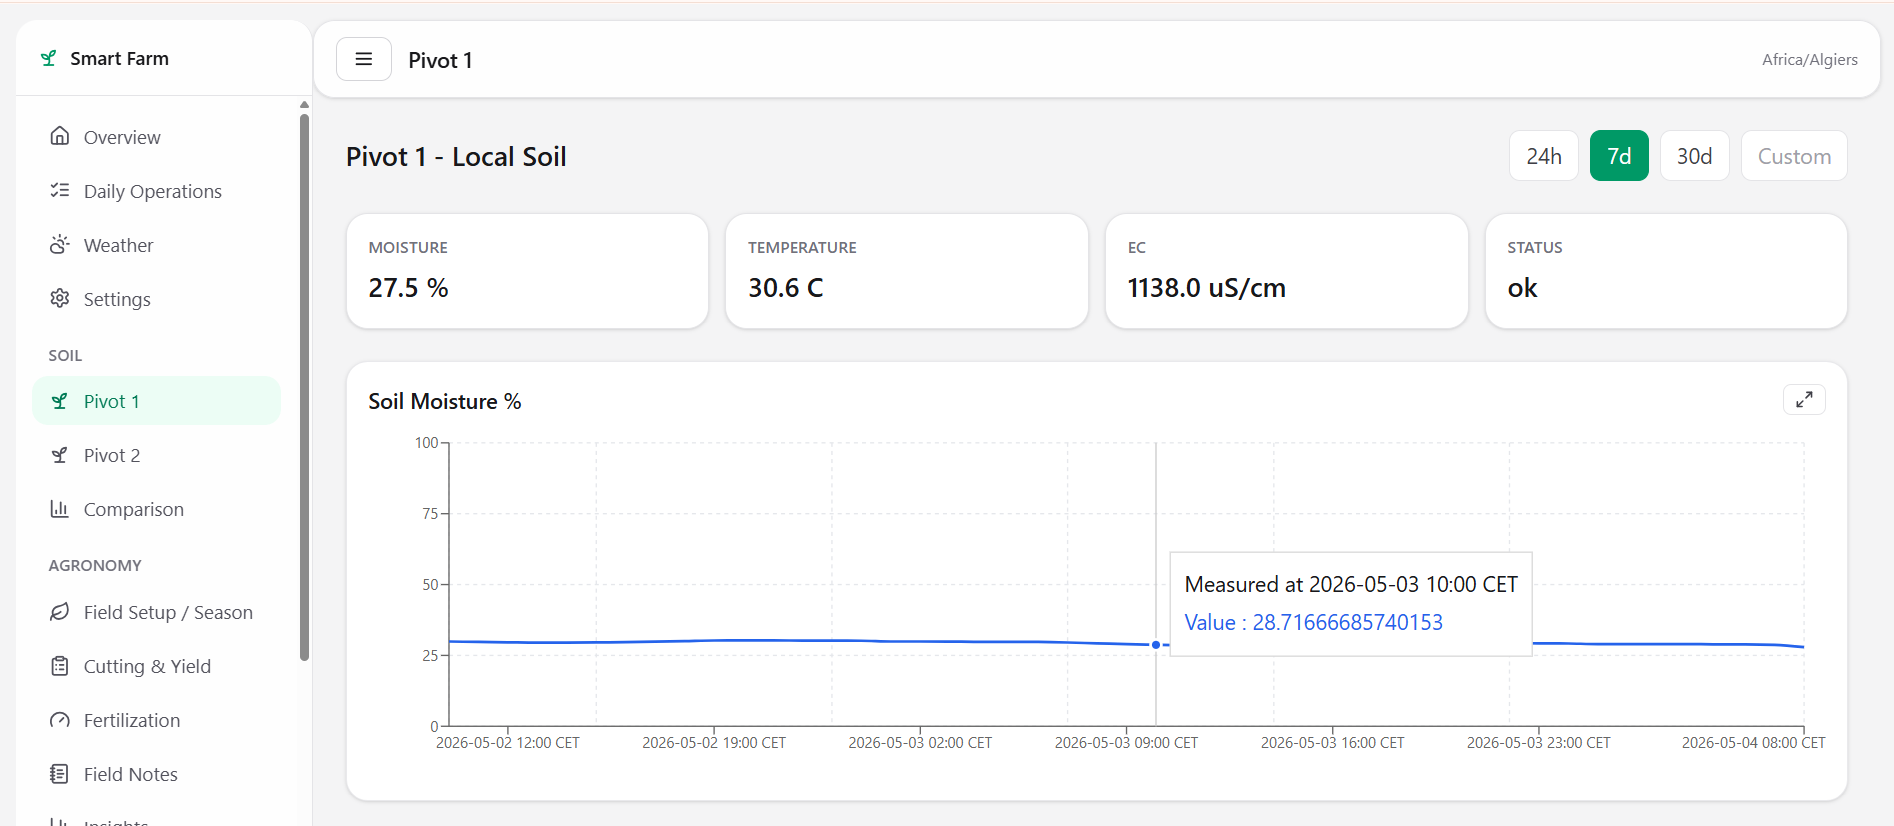
\includegraphics[width=\textwidth]{figures/DashPivot}
% TODO: copy Academic-Thesis/DashBoredImages/Pivot.png to figures/DashPivot.png before compiling
\caption{Pivot soil monitoring page displaying soil moisture, temperature, and electrical conductivity trends from Node2 (Pivot~2 remote soil sensor), with time axis derived from \texttt{measured\_at} timestamps.}
\label{fig:pivot-soil-dashboard}
\end{figure}

The pivot soil monitoring page presents time-series charts for the soil measurement dimensions: moisture, temperature, and EC. Chart time axes are populated from the \texttt{measured\_at} field in the \texttt{sensor\_readings} table, consistent with the time policy established in Section~\ref{sec:storage-time}. The upload timestamp is not used as a chart axis value at any point in the rendering pipeline.

\begin{figure}[H]
\centering
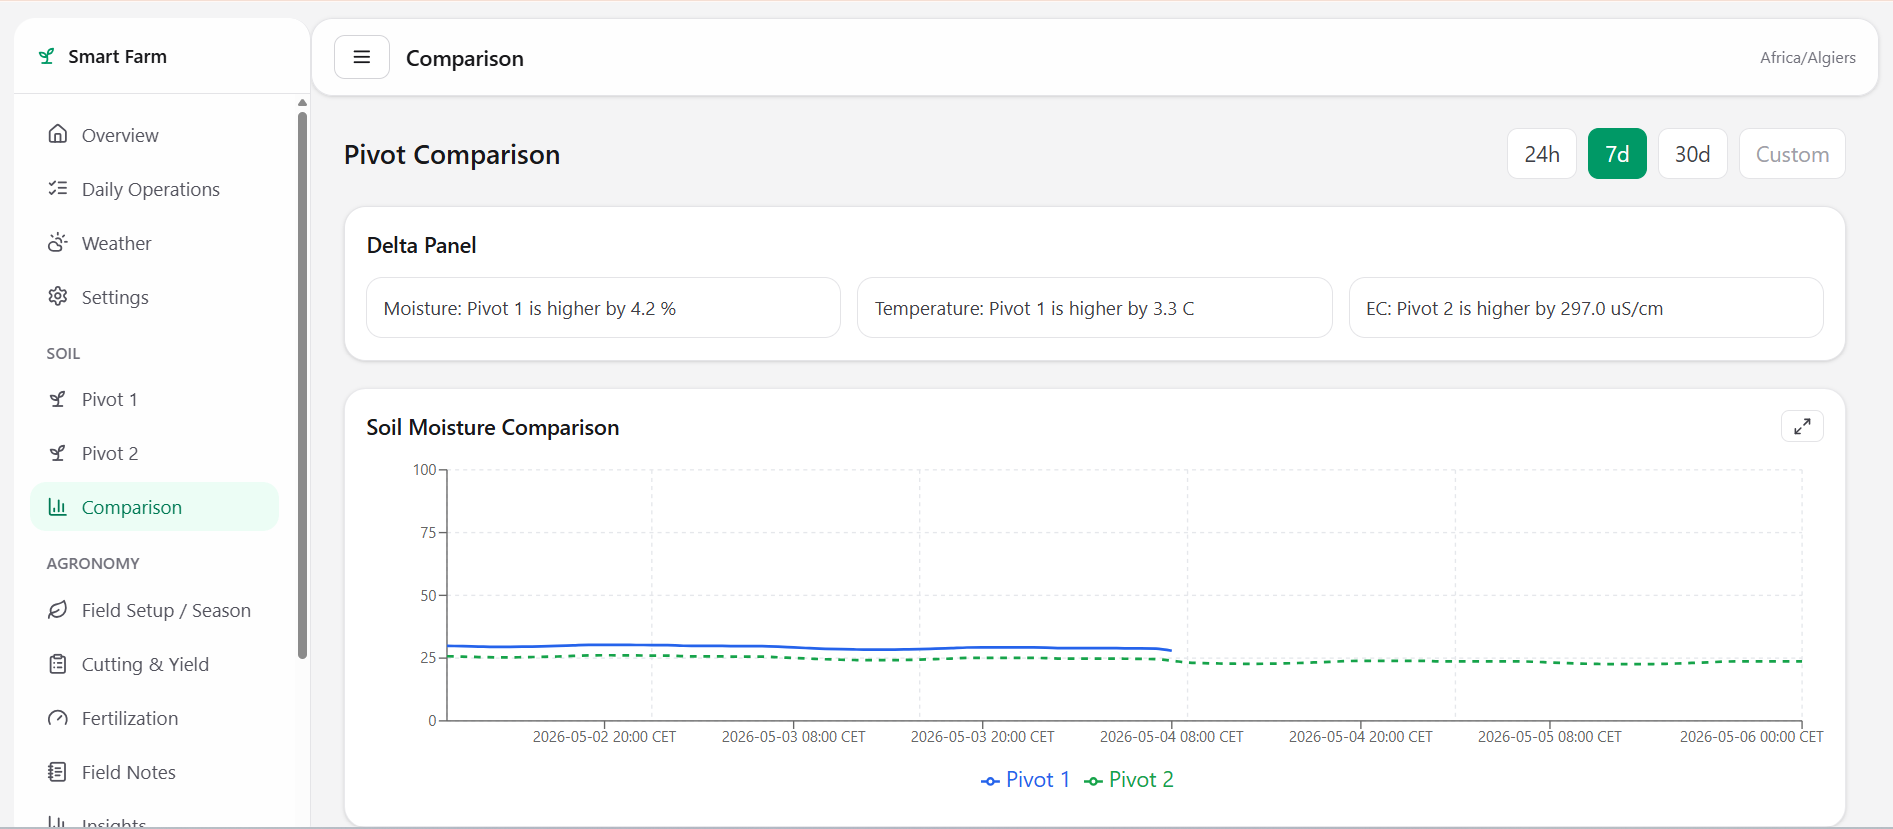
\includegraphics[width=\textwidth]{figures/DashComparison}
% TODO: copy Academic-Thesis/DashBoredImages/Comparison.png to figures/DashComparison.png before compiling
\caption{Pivot comparison page presenting side-by-side soil metric trends for Pivot~1 and Pivot~2, supporting the identification of differences in soil response between the two irrigation zones.}
\label{fig:pivot-comparison-dashboard}
\end{figure}

The pivot comparison page places soil data from both irrigation locations on aligned time axes, enabling the operator to compare the soil response of Pivot~1 and Pivot~2 under the same temporal frame. Because the two nodes collect independent soil measurements at physically distinct locations, the comparison supports irrigation management decisions rather than serving as a redundancy check.

\begin{figure}[H]
\centering
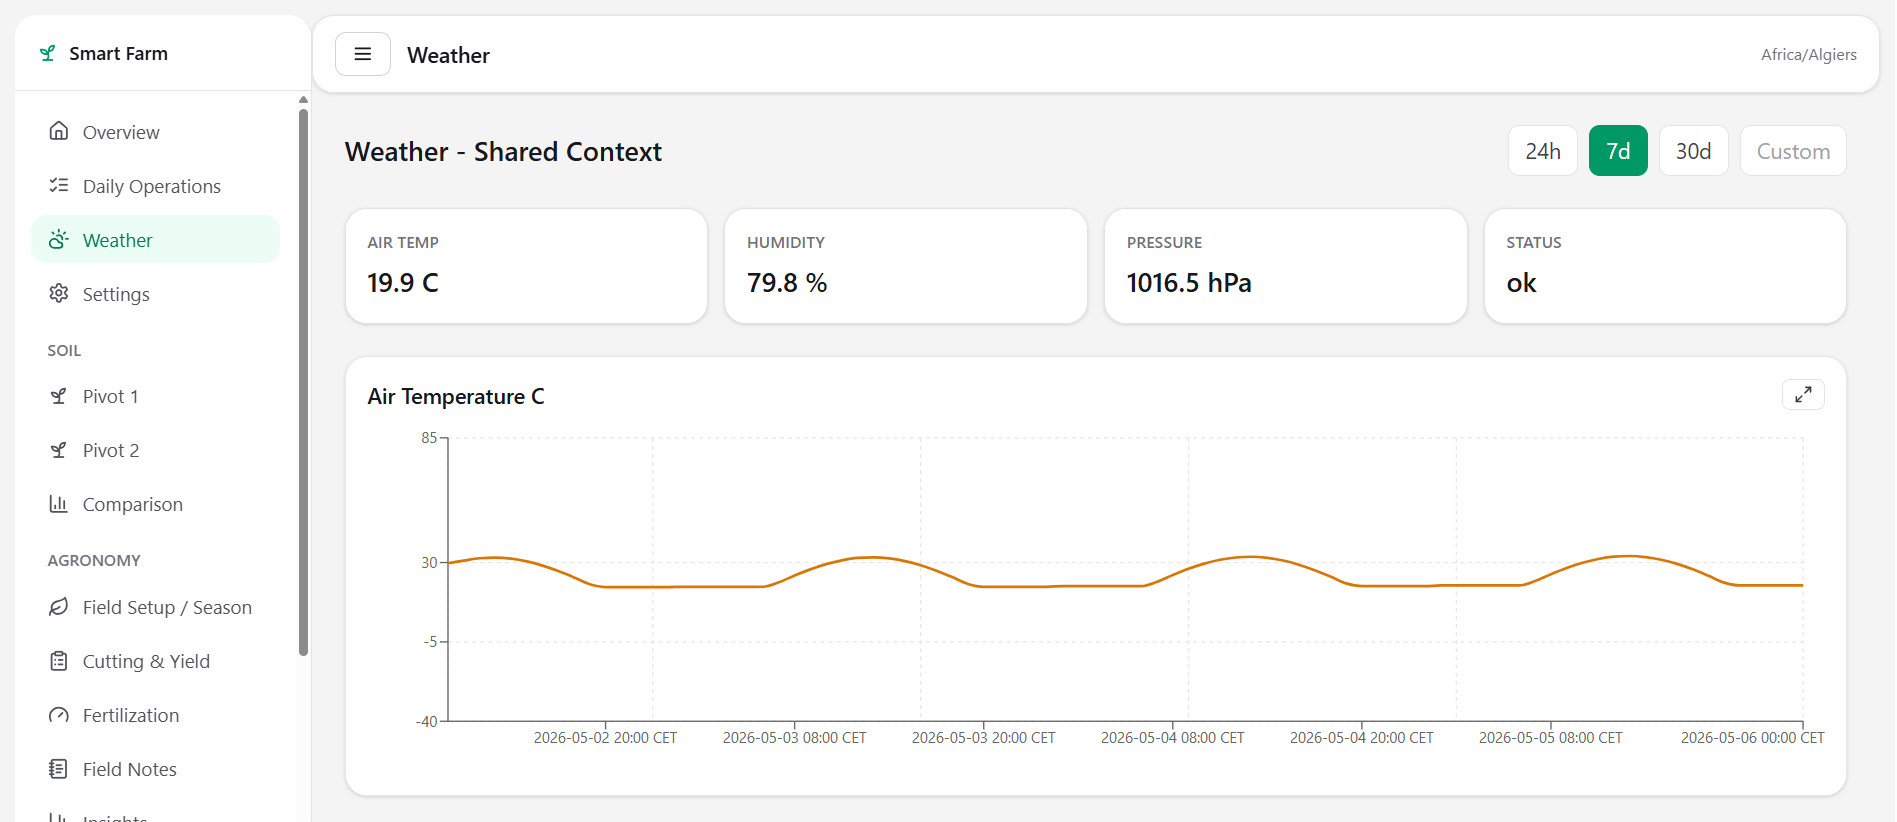
\includegraphics[width=\textwidth]{figures/DashWeather}
% TODO: copy Academic-Thesis/DashBoredImages/Weather.png to figures/DashWeather.png before compiling
\caption{Weather monitoring page presenting air temperature, relative humidity, and barometric pressure time series from Node3.}
\label{fig:weather-dashboard}
\end{figure}

The weather page displays the three atmospheric parameters provided by Node3: air temperature, relative humidity, and barometric pressure. These measurements provide agronomic context for interpreting soil moisture trends and are presented on the same measurement-time axis as the soil charts, preserving temporal alignment across the monitoring domains.

\begin{figure}[H]
\centering
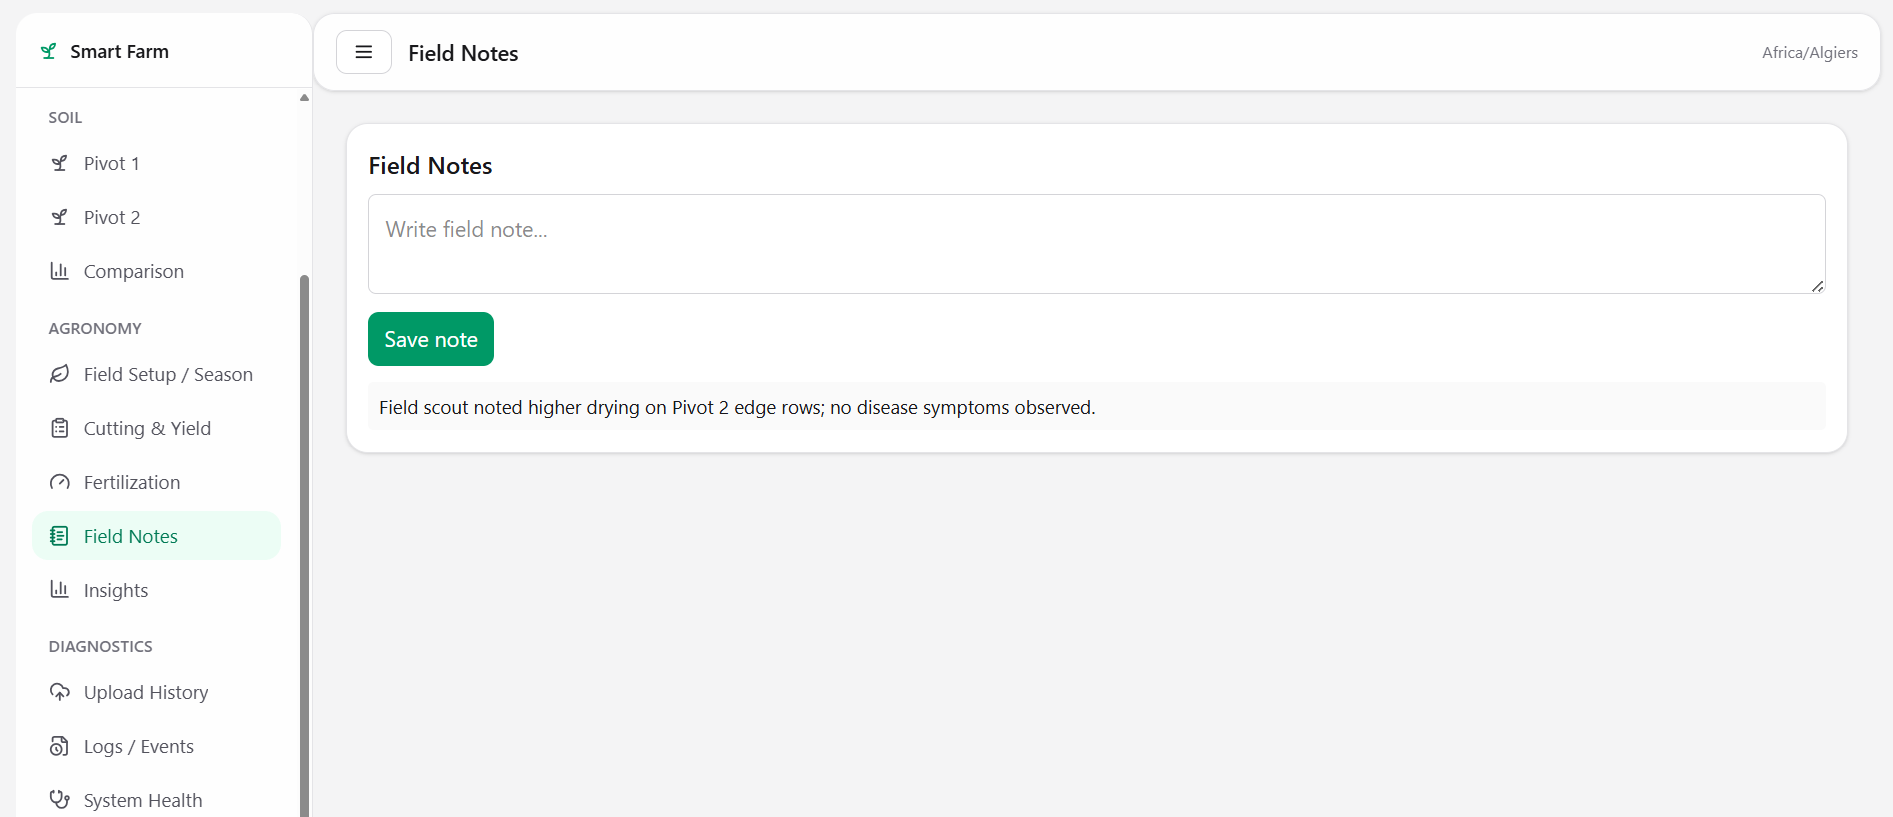
\includegraphics[width=\textwidth]{figures/DashFieldNotes}
% TODO: copy Academic-Thesis/DashBoredImages/FieldNotes.png to figures/DashFieldNotes.png before compiling
\caption{Field notes and agronomic events page listing manually recorded irrigation sessions, fertilisation applications, and field observations, with start and end times stored in the \texttt{agronomic\_events} table.}
\label{fig:field-notes-dashboard}
\end{figure}

The field notes page presents the \texttt{agronomic\_events} table in a chronological list, exposing operator-entered records of irrigation sessions, fertilisation applications, and field observations. These records are stored independently of the sensor reading domain and are overlaid on soil moisture charts to provide interpretive context. The interface does not interpret or annotate agronomic events automatically; the operator supplies all semantic meaning through the event type and notes fields at the time of entry.

% ============================================================
\section{Deterministic Analytics Layer}
\label{sec:analytics}
% ============================================================

The deterministic analytics layer is the computational engine of the platform. It operates on uploaded sensor readings to produce quality-controlled, reliability-scored, and alert-evaluated outputs that are stored as analytics snapshots and presented to the operator through the Insights and Processed Data Viewer pages. The layer is deterministic: given the same input readings, quality flags, and configured thresholds, it produces the same output every time. Gemini does not participate in any stage of this pipeline; AI-generated narratives are prepared only after the deterministic outputs have been computed and stored.

\begin{figure}[H]
\centering
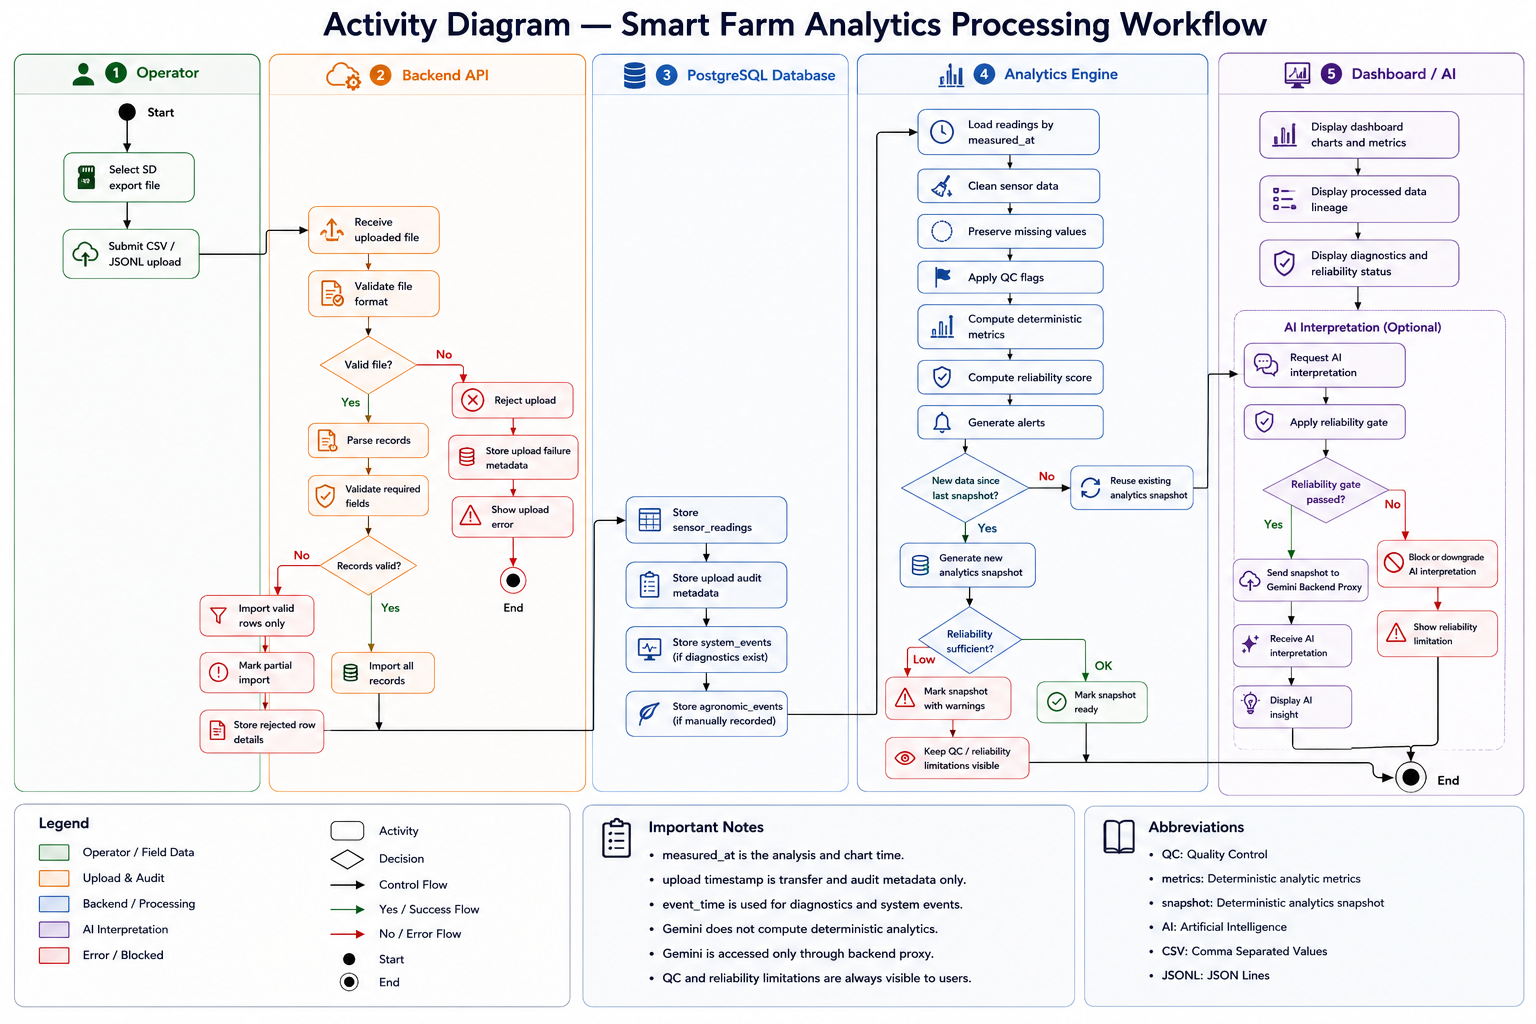
\includegraphics[width=0.90\textwidth]{figures/ActivityDiagram}
% TODO: copy Academic-Thesis/Diagrams/Activity Diagram.png to figures/ActivityDiagram.png before compiling
\caption{Activity diagram of the deterministic analytics pipeline, showing the sequence from raw sensor readings through timestamp validation, duplicate detection, range and flatline checking, quality scoring, reliability scoring, alert evaluation, and analytics snapshot generation.}
\label{fig:deterministic-analytics-workflow}
\end{figure}

The pipeline proceeds through ten ordered stages. Raw sensor readings enter from the \texttt{sensor\_readings} table. Each stage applies a rule set and passes annotated records to the next stage; no stage modifies the stored sensor values — quality flags and derived metrics are maintained separately. Table~\ref{tab:analytics-pipeline} describes each stage in detail.

\begin{table}[H]
\centering
\caption{Stages of the deterministic analytics pipeline, showing inputs, processing roles, outputs, and safety boundaries at each stage.}
\label{tab:analytics-pipeline}
\small
\begin{tabular}{p{2.8cm} p{2.5cm} p{3.0cm} p{2.8cm} p{2.5cm}}
\hline
\textbf{Stage} & \textbf{Input} & \textbf{Processing role} & \textbf{Output} & \textbf{Safety boundary} \\
\hline
Canonical timestamp check & Raw readings & Verify \texttt{measured\_at} is present and in UTC; normalise timezone representation & Timestamp-validated set & Records without \texttt{measured\_at} are excluded, not corrected \\
\hline
Duplicate detection & Timestamp-validated set & Identify records sharing the same node and \texttt{measured\_at} within tolerance & Deduplicated set with duplicate flags & Originals preserved; duplicates flagged, not deleted \\
\hline
Missing data analysis & Deduplicated set & Count and characterise gaps per measurement window & Gap map per node and domain & Values are never imputed; gaps remain visible \\
\hline
Physical range checking & Sensor readings & Compare values against physical bounds for each measurement type & Range-flagged annotations & No automatic value correction; operator-visible flag only \\
\hline
Flatline and spike detection & Range-checked readings & Statistical consistency checks across consecutive readings & Quality-flagged annotations & Suspect readings remain in the dataset with flags; not silently removed \\
\hline
System-event cross-reference & Quality flags + system events & Align diagnostic events with the measurement window & Event-aligned quality annotations & Does not override QC flags; adds context only \\
\hline
Window quality scoring & Quality flags + agronomic event confidence & Compute a weighted quality metric per time window & Window quality score & Agronomic event confidence weighting is additive; does not suppress low-quality flags \\
\hline
Node reliability scoring & Window quality scores + upload metadata & Aggregate per-node reliability across the analysis window & Node reliability indicator & Upload freshness affects score; low reliability remains exposed, not normalised \\
\hline
Deterministic alert evaluation & Reliability score + quality flags & Evaluate configured threshold conditions & Alert records & No AI involvement; thresholds are operator-configured values \\
\hline
Analytics snapshot & All stage outputs & Aggregate quality score, reliability, alerts, and limitations into a \texttt{analytics\_snapshots} record & Snapshot stored in PostgreSQL & This snapshot — not raw data — is the only input forwarded to the Gemini proxy \\
\hline
\end{tabular}
\end{table}

Two additional inputs feed into the quality and reliability stages. Agronomic events recorded in the \texttt{agronomic\_events} table contribute a confidence weight to the window quality scoring stage, reflecting the principle that a window accompanied by a recorded irrigation or fertilisation event carries stronger interpretive context. Upload metadata from the \texttt{uploads} table informs the upload freshness diagnostic component of node reliability scoring.

\begin{figure}[H]
\centering
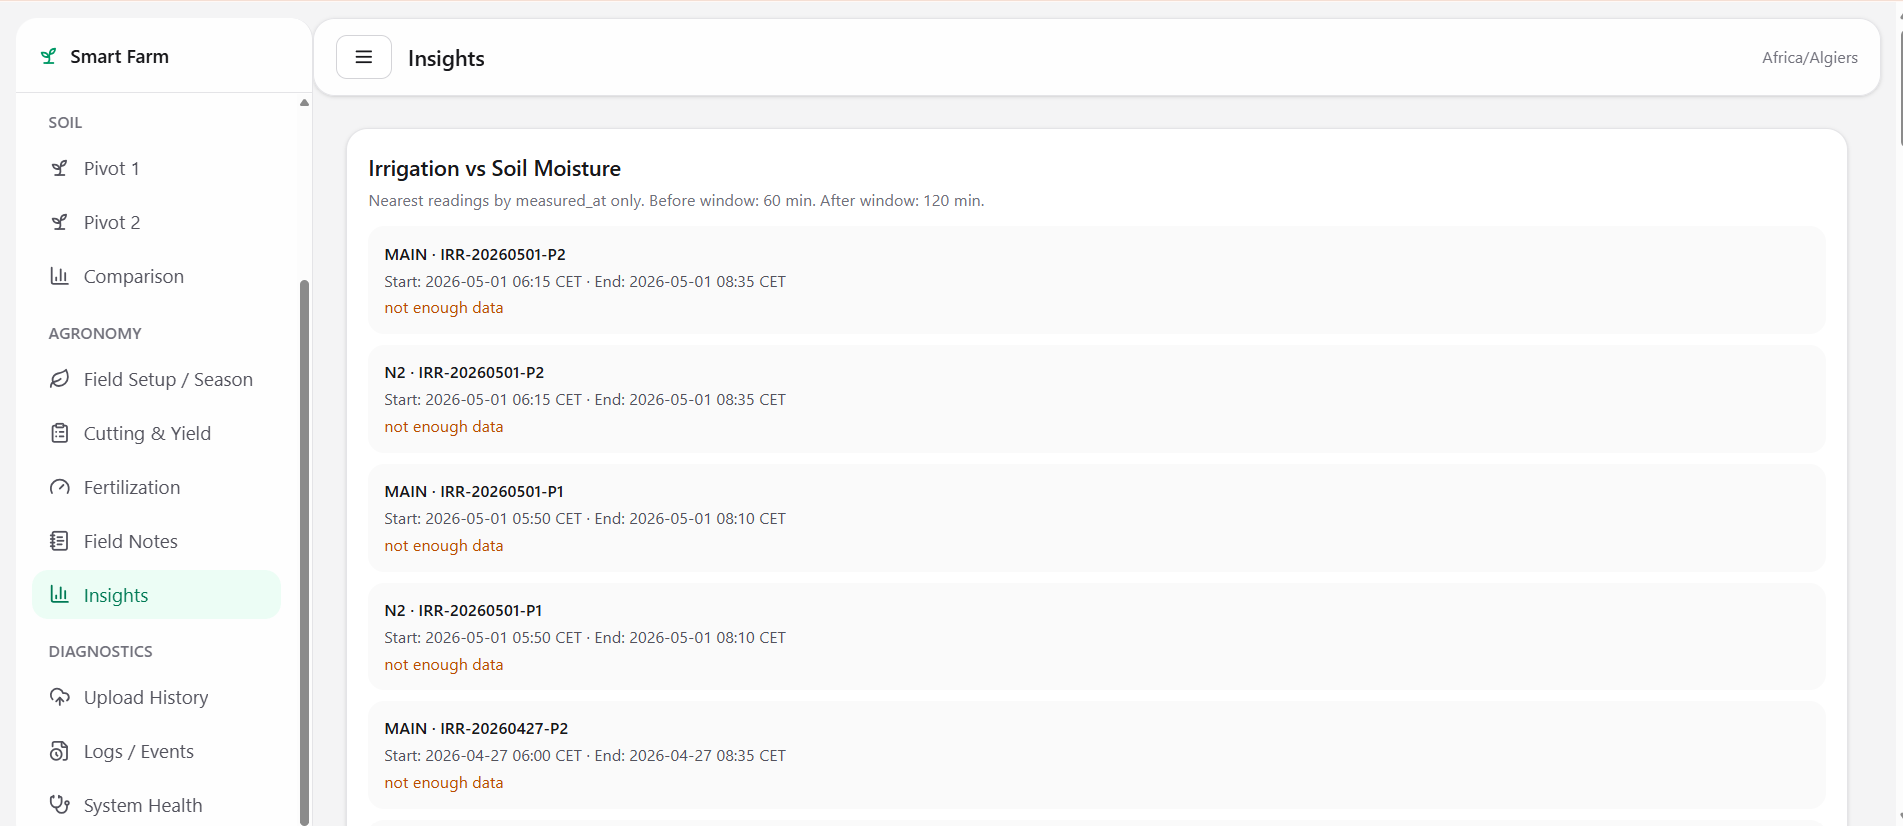
\includegraphics[width=\textwidth]{figures/DashInsights}
% TODO: copy Academic-Thesis/DashBoredImages/Insights.png to figures/DashInsights.png before compiling
\caption{Analytics Insights page displaying deterministic quality scores, reliability indicators, and alert summaries derived from the analytics pipeline. AI-generated narratives appear in a separate, clearly labelled panel.}
\label{fig:insights-dashboard}
\end{figure}

The Insights page presents the outputs of the deterministic pipeline alongside any AI-generated narrative that has been requested for the current analytics snapshot. The deterministic metrics — quality score, reliability indicator, and alert list — are displayed in the primary panel. The AI narrative appears in a secondary panel with a visual label identifying it as an AI-generated interpretation. The physical separation reinforces the principle that deterministic analytics are the authoritative layer and AI narratives are supplementary decision-support information.

% ============================================================
\section{Processed Data Viewer}
\label{sec:processed-data-viewer}
% ============================================================

The Processed Data Viewer is a read-only transparency interface that exposes the full output of the deterministic analytics pipeline for a selected time window. Its purpose is to allow the operator — and, in an academic context, the reviewer — to inspect the lineage from raw sensor readings through each processing stage to the final quality-annotated result.

\begin{figure}[H]
\centering
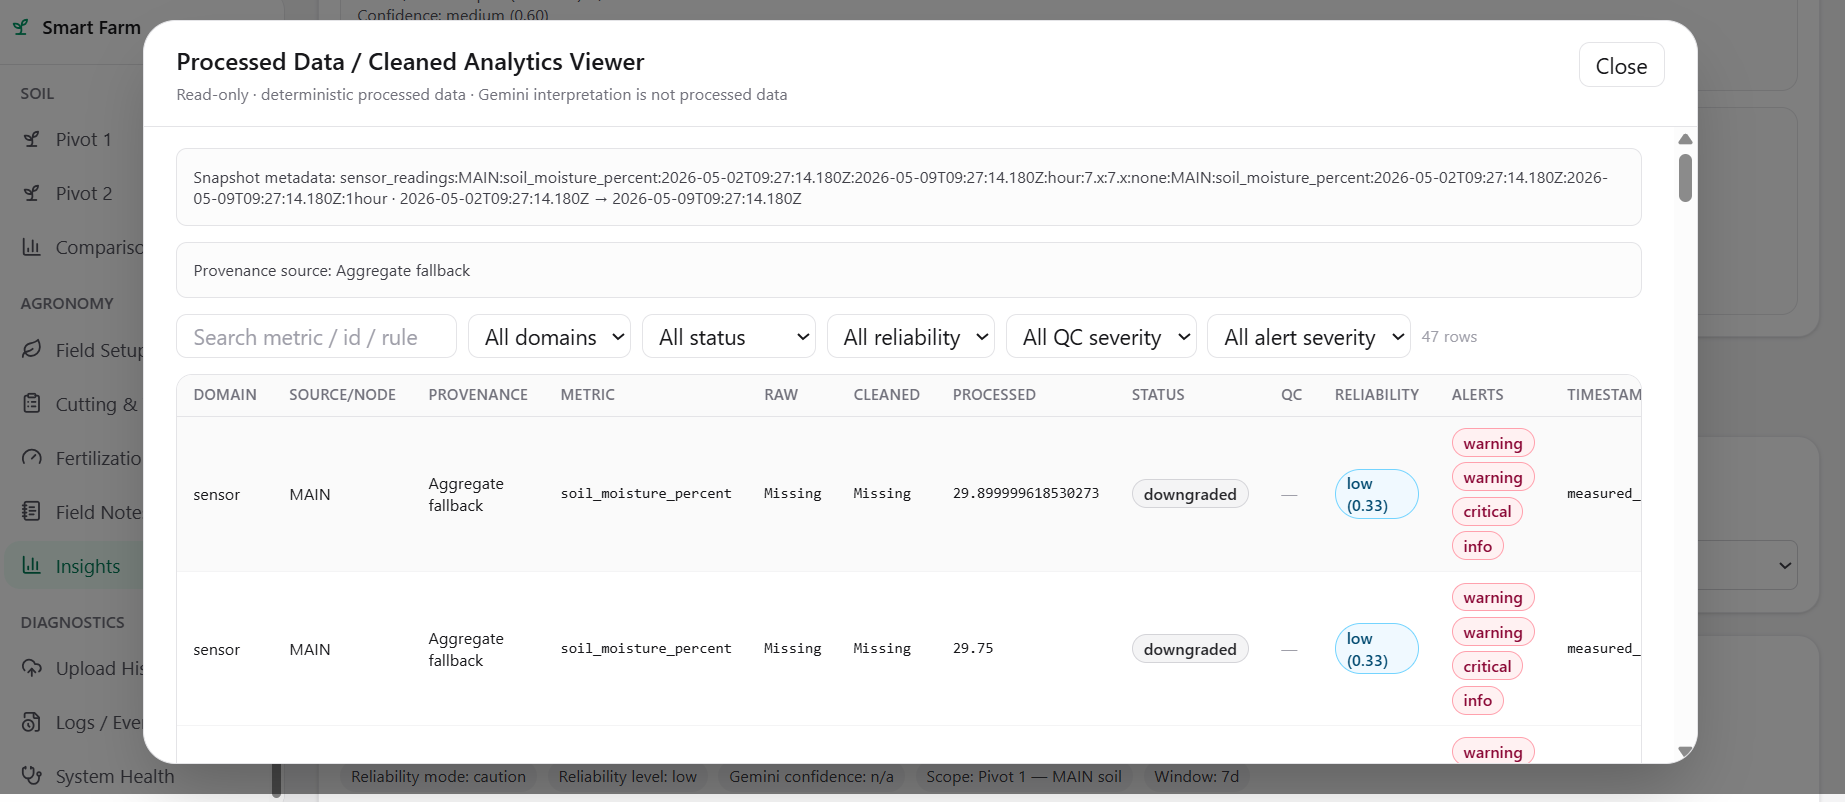
\includegraphics[width=\textwidth]{figures/ProcessedData}
% TODO: The source file is Academic-Thesis/DashBoredImages/ProcessedData .png — note the space before the extension. Rename to ProcessedData.png before copying to figures/ProcessedData.png, or escape the space in the LaTeX path if the toolchain supports it.
\caption{Processed Data Viewer page showing the output of the deterministic analytics pipeline for the selected analysis window, including per-record quality flags, reliability indicator, deterministic alert references, and a safe export function.}
\label{fig:processed-data-viewer}
\end{figure}

The viewer presents the output of the \texttt{analytics\_snapshots} table for the selected window. For each processed record, it exposes the raw input values, the quality flags applied at each pipeline stage, the window quality score, the node reliability indicator, any deterministic alerts that were triggered, and any limitations attached to the record. The viewer does not expose an editing interface; all values are read-only, and the raw sensor readings in the \texttt{sensor\_readings} table are not modified by the analytics pipeline at any stage.

A safe export function allows the operator to download the processed data in a portable format for offline analysis or academic reporting. The exported file includes the processing lineage columns alongside the sensor values, preserving the full context needed to reproduce the quality assessment independently.

% ============================================================
\section{AI Interpretation Layer}
\label{sec:ai-interpretation}
% ============================================================

The AI interpretation layer provides narrative context to support operator decision-making. It is implemented as a backend-proxied interface to the Gemini generative AI model. The layer is deliberately constrained: it operates downstream of the deterministic analytics pipeline, receives only the processed analytics snapshot, and produces narrative text that is presented to the operator alongside — not in place of — the deterministic outputs.

\begin{figure}[H]
\centering
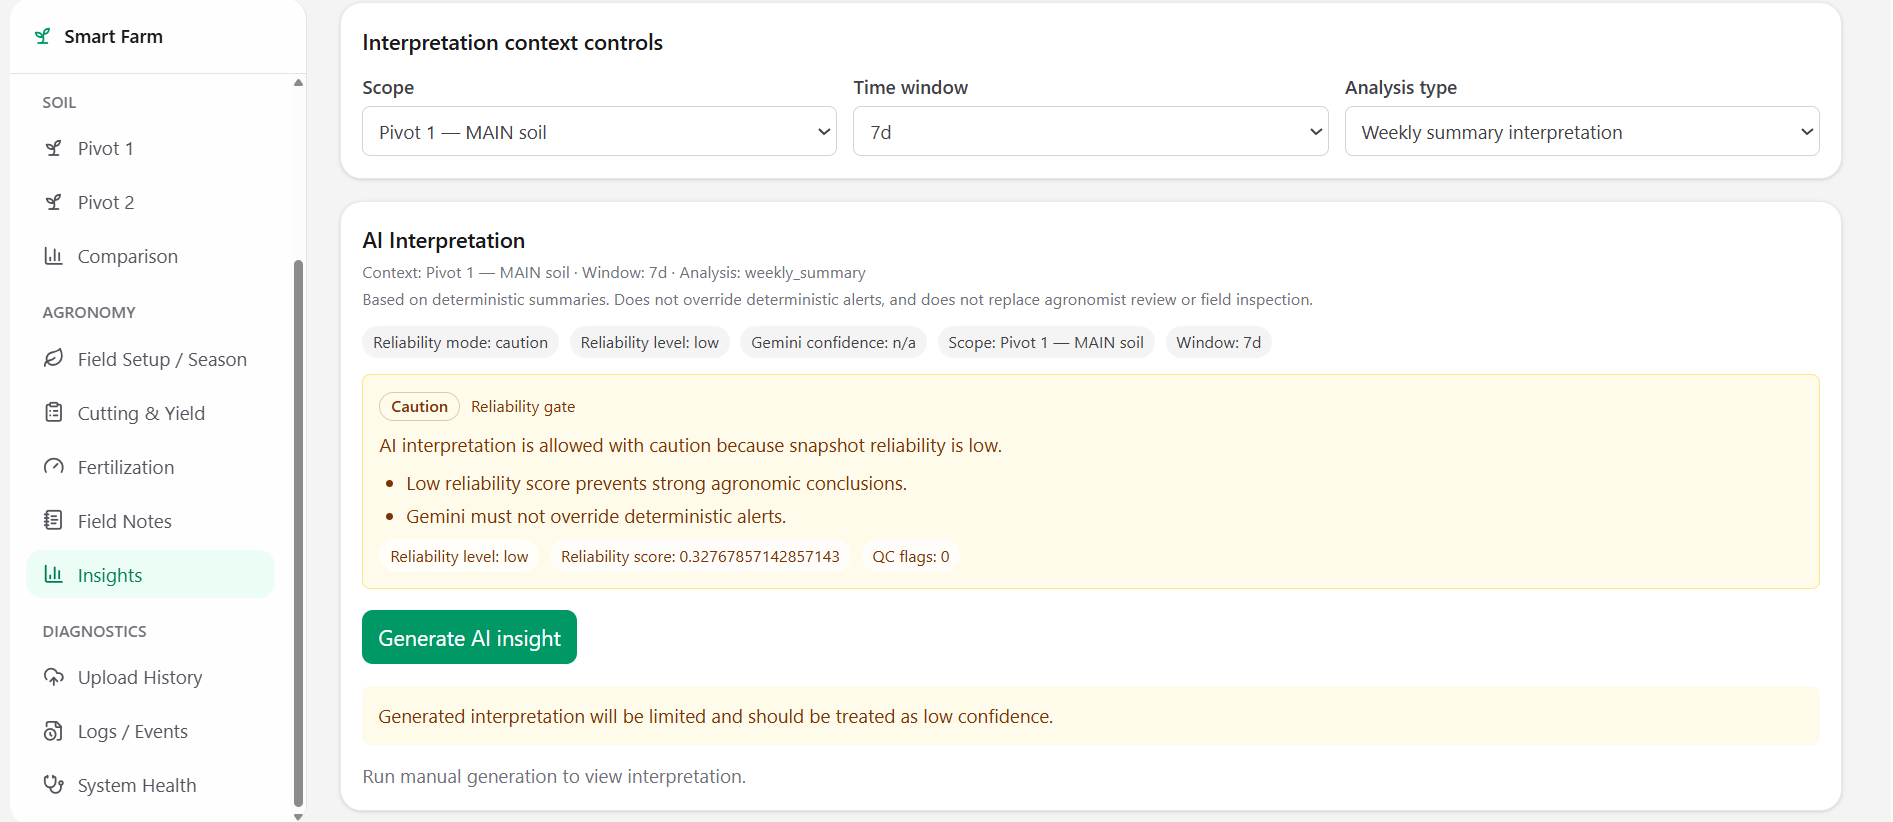
\includegraphics[width=\textwidth]{figures/DashAiInsight}
% TODO: copy Academic-Thesis/DashBoredImages/AiInsight.png to figures/DashAiInsight.png before compiling
\caption{AI Insight page presenting a Gemini-generated narrative interpretation of the current analytics snapshot. The deterministic metrics, reliability indicator, and QC flags are passed as context; the AI response is labelled as an interpretive narrative and presented separately from the deterministic layer.}
\label{fig:ai-interpretation-ui}
\end{figure}

The boundary governing the AI layer is defined at six levels, described in Table~\ref{tab:ai-boundary}. Each boundary addresses a specific risk: data integrity, metric reproducibility, scope control, user misinterpretation, and the agronomist principle established in Chapter~\ref{chap:related-works}.

\begin{table}[H]
\centering
\caption{AI interpretation boundary rules, their implementation, and rationale.}
\label{tab:ai-boundary}
\small
\begin{tabular}{p{3.5cm} p{5.0cm} p{5.0cm}}
\hline
\textbf{Boundary rule} & \textbf{Implementation meaning} & \textbf{Reason} \\
\hline
Backend proxy only & Gemini API calls are routed exclusively through the WebService backend; the dashboard frontend never calls the Gemini API directly & Prevents raw sensor data, database content, and API credentials from being exposed at the client layer \\
\hline
Snapshot input only & Gemini receives the deterministic analytics snapshot; it does not receive raw \texttt{sensor\_readings} rows, individual reading objects, or direct database query results & Constrains AI interpretation scope to validated, quality-annotated output rather than unprocessed measurements \\
\hline
No raw data mutation & Gemini cannot write to the database, modify reading values, fill missing values, alter QC flags, or change alert severity & Preserves the integrity of the sensor record and the reproducibility of the deterministic pipeline \\
\hline
No metric computation & Quality scores, reliability indicator, and alert evaluation are computed deterministically before Gemini is invoked; Gemini is not asked to recompute or validate any metric & Ensures primary analytics are reproducible from project code, not dependent on AI model state \\
\hline
Reliability gate & A reliability threshold check is applied before the snapshot is forwarded; a low-confidence snapshot triggers an operator-visible warning before AI interpretation is requested & Prevents AI narrative from appearing normal when underlying data quality is insufficient \\
\hline
Human decision final & AI-generated narratives are presented as decision-support information; agronomic decisions remain with the human operator & Consistent with the monitoring-only scope of the system and the agronomist boundary established in Section~\ref{sec:proposed-improvements} \\
\hline
\end{tabular}
\end{table}

The \texttt{/api/v1/gemini} endpoint enforces all six boundaries in a single processing function. The function retrieves the analytics snapshot, evaluates the reliability gate, constructs a structured prompt containing the snapshot context and the system's declared constraints, forwards the prompt to the Gemini API, and returns the narrative response to the dashboard. The response is never stored in the \texttt{sensor\_readings}, \texttt{system\_events}, or \texttt{analytics\_snapshots} tables; it exists only as a transient response for the current session.

% ============================================================
\section{Field Deployment}
\label{sec:deployment}
% ============================================================

The system was assembled and deployed as a field-oriented prototype for monitoring alfalfa cultivation in the El~Oued region of Algeria. The deployment context is consistent with the Saharan agricultural environment described in Section~\ref{sec:saharan-agriculture}: intermittent power availability, no permanent Internet connection at the field site, and a need for autonomous data acquisition across multi-day periods between operator visits.

The three nodes described in Section~\ref{sec:hardware} were mounted and positioned according to their sensing roles. The MAIN gateway was installed at the Pivot~1 location, providing both LoRa reception coordination and local soil monitoring for the first irrigation zone. Node2 was deployed at the Pivot~2 location, independently acquiring soil measurements for the second irrigation zone and transmitting them to MAIN over LoRa. Node3 was positioned as a dedicated weather station, collecting atmospheric parameters over the full deployment window.

Node operation during the deployment follows the manual workflows described in Sections~\ref{sec:mode-upload} and~\ref{sec:mode-rtc-sync}. The operator visits the field site with an Internet connection periodically, connects the MAIN node to the available network, and activates Upload Mode with a sustained button press to transfer accumulated SD content to the backend. RTC synchronisation is performed with four consecutive button presses before the upload session if clock drift is suspected. Between operator visits, the three nodes cycle through the ten-minute superframe independently, storing measurements locally on the MAIN SD card without any network dependency.

The three nodes were housed in protective enclosures rated IP65, providing resistance to dust ingress and water contact from all directions. In the Saharan field context, this rating addresses the primary environmental risks to embedded electronics: wind-borne fine sand and dust, periodic humidity, and incidental mechanical contact during maintenance visits. The IP65 rating does not imply submersion tolerance; the nodes are not waterproof to immersion. Figures~\ref{fig:field-main-node-deployment}, \ref{fig:field-node2-soil-enclosure}, and~\ref{fig:field-node3-weather-enclosure} document the three deployed nodes in their respective field positions.

\begin{figure}[H]
\centering
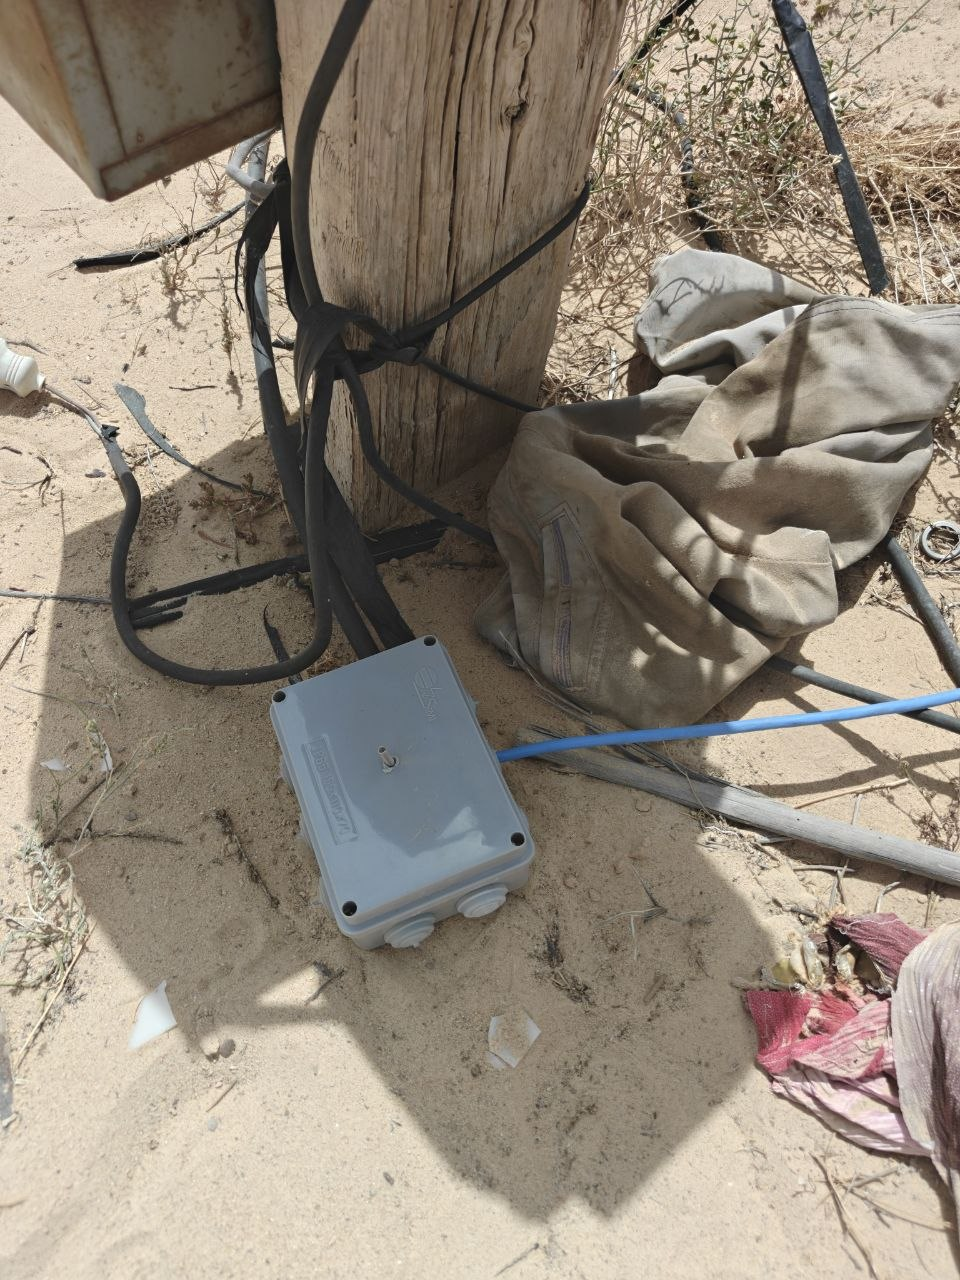
\includegraphics[width=0.72\textwidth]{figures/field-main-node-deployment}
\caption{MAIN gateway node at the Pivot~1 field location during the pilot deployment. The IP65-rated enclosure provides dust and water-contact resistance appropriate for outdoor Saharan field conditions. The node operates on battery power. Electrical infrastructure visible in the surrounding area belongs to the existing field site; it does not serve as the node power source.}
\label{fig:field-main-node-deployment}
\end{figure}

\begin{figure}[H]
\centering
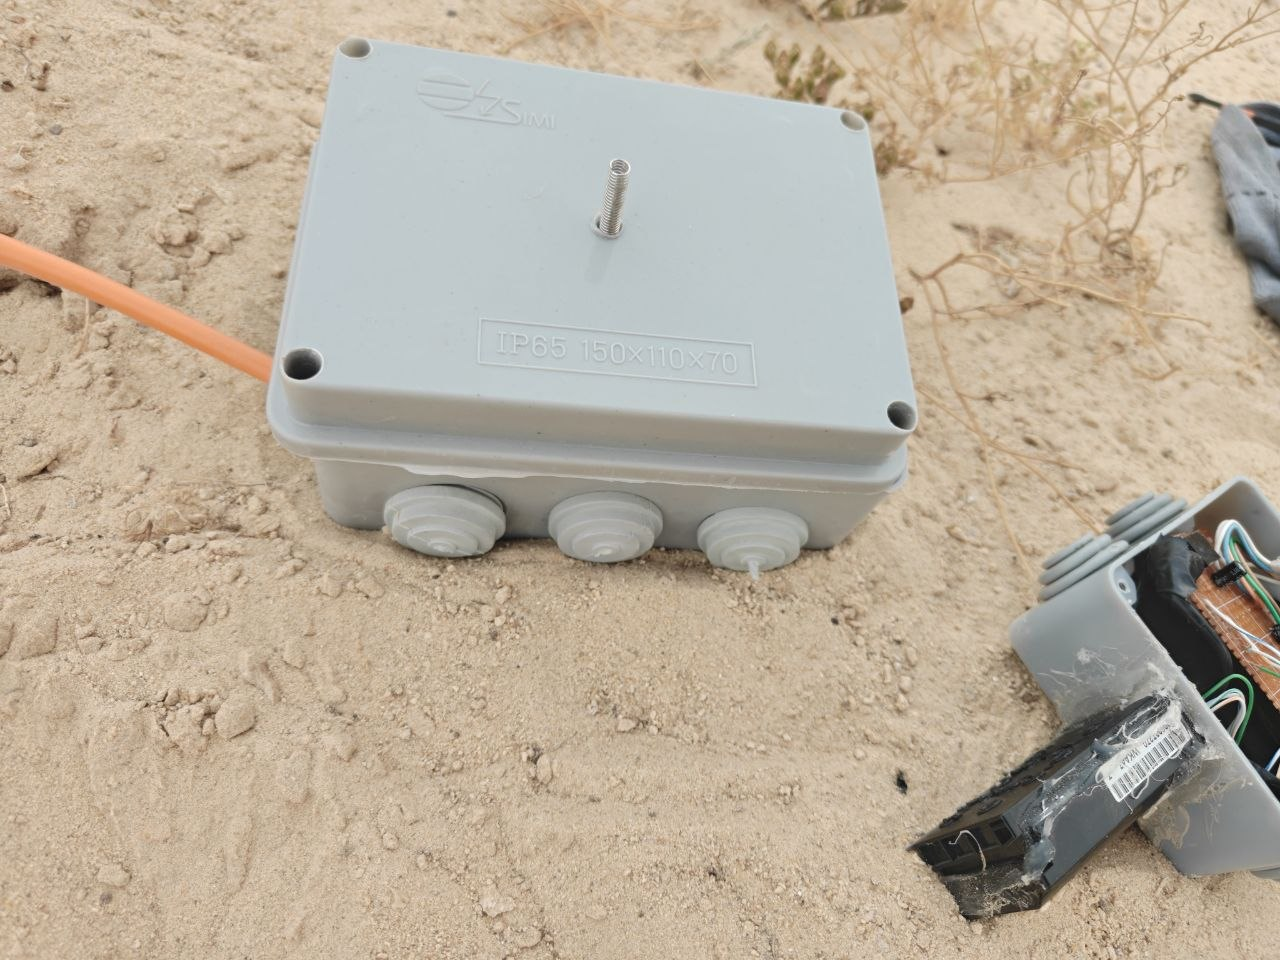
\includegraphics[width=0.72\textwidth]{figures/field-node2-soil-enclosure}
\caption{Node2 soil sensing enclosure at the Pivot~2 field location. A CAT6 RJ45 outdoor cable connects the enclosure to the in-ground RS485 soil sensor, carrying the sensor signal and power conductors required by the Modbus soil sensing interface. The cable was selected for its outdoor insulation, humidity and soil-contact resistance, reliable copper conductors, and multi-conductor configuration; it functions as a utility signal cable in this application, not as an Ethernet connection.}
\label{fig:field-node2-soil-enclosure}
\end{figure}

\begin{figure}[H]
\centering
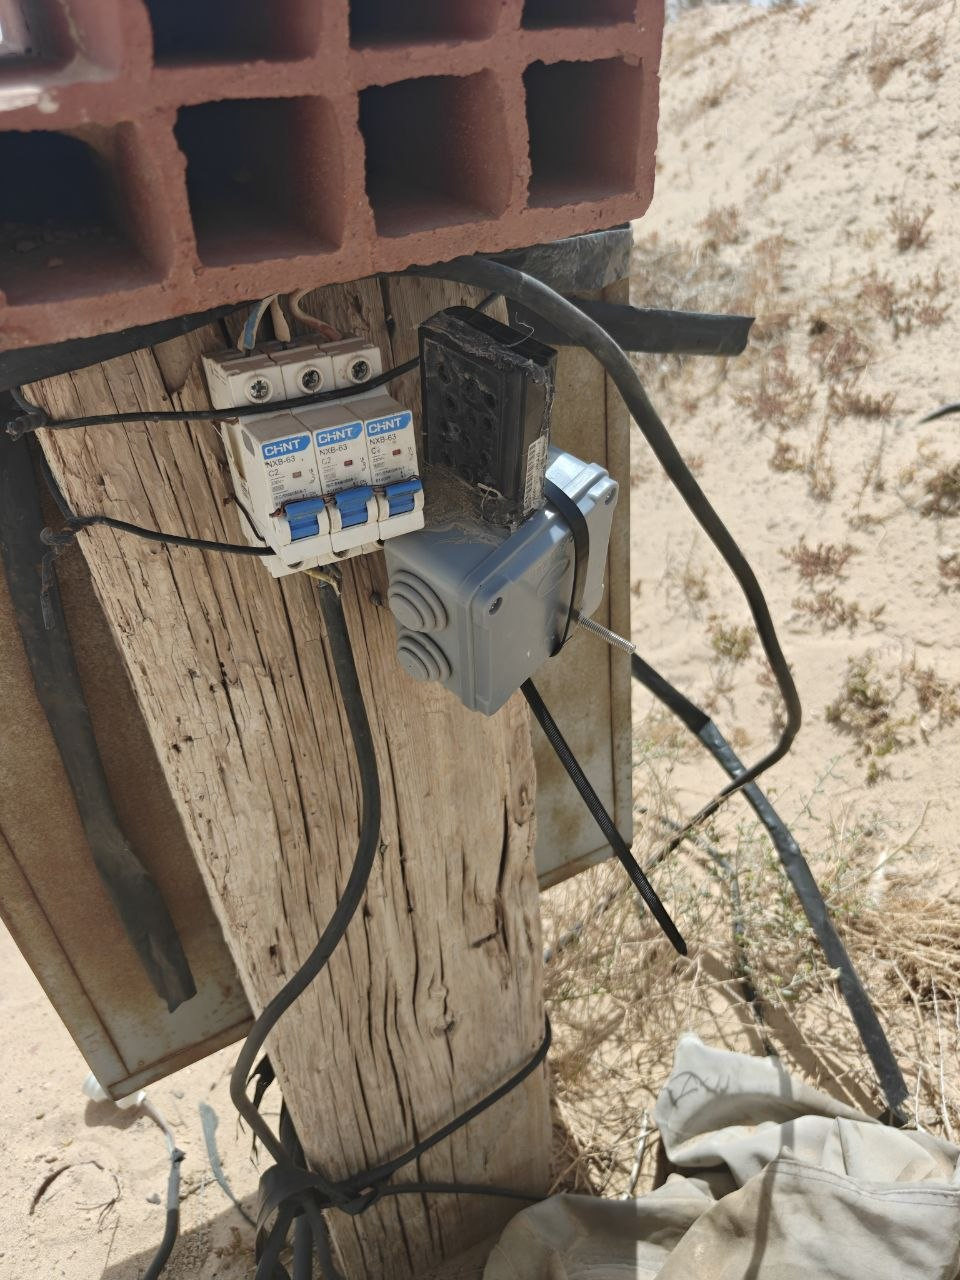
\includegraphics[width=0.72\textwidth]{figures/field-node3-weather-enclosure}
\caption{Node3 weather sensing node at its field position during the pilot validation window. The IP65-rated enclosure houses the ESP32-C3, LoRa transceiver, and BME280 sensor, providing dust and water-contact protection suitable for outdoor atmospheric monitoring in a Saharan environment.}
\label{fig:field-node3-weather-enclosure}
\end{figure}

The deployment does not constitute a formal long-term field trial. The evidence presented in this chapter spans a 5.5-day validation window from 2026-05-06 to 2026-05-11, during which the system operated across six upload sessions. This window demonstrates functional feasibility and the end-to-end operation of the sensing, storage, upload, and analytics pipeline. Long-term robustness, seasonal measurement coverage, and calibrated agronomic threshold validation are identified as future work in Section~\ref{sec:limitations}.

% ============================================================
\section{Data Analysis and Results}
\label{sec:results}
% ============================================================

The data presented in this section were acquired during the pilot validation window from 2026-05-06 00:00~UTC to 2026-05-11 15:00~UTC. All measurements originate from the sensor nodes and were transferred to the backend across six upload sessions. The analysis is bounded by the available evidence and is intended to demonstrate functional feasibility of the data acquisition, storage, transfer, and processing pipeline — not to draw calibrated agronomic conclusions.

\begin{table}[H]
\centering
\caption{Summary of validation dataset evidence, observed values, and interpretation scope.}
\label{tab:validation-data-summary}
\small
\begin{tabular}{p{3.5cm} p{3.5cm} p{6.5cm}}
\hline
\textbf{Evidence item} & \textbf{Value} & \textbf{Interpretation} \\
\hline
Sensor readings & 2433 total & 811 records per node (MAIN, N2, N3); equal distribution confirms superframe-level consistency across the validation window \\
\hline
Missing \texttt{measured\_at} & 0 rows & Every reading carries a canonical measurement timestamp; timestamp policy enforced at ingestion \\
\hline
Reading status & All \texttt{ok} & No ingestion-level rejection within the provided dataset; status reflects database record state \\
\hline
System events & 8 & Logged from 2026-05-08 to 2026-05-11; include node-missing events, an irrigation-completed record, and a heat-stress warning \\
\hline
Agronomic events & 6 & Four irrigation sessions (Pivot~1 and Pivot~2 on 2026-05-08 and 2026-05-11), one fertilisation application (2026-05-10), one field scouting note (2026-05-09) \\
\hline
Upload sessions & 6 & All sessions reached \texttt{processed} status; three upload anomalies recorded in one session \\
\hline
Processed data rows & 135 & Output of the deterministic analytics pipeline for the analysis window; reliability indicator uniform at 0.399 across all rows \\
\hline
Validation window & 5 days 15 hours & Pilot validation window; functional feasibility scope only — not full-season agronomic validation \\
\hline
\end{tabular}
\end{table}

Table~\ref{tab:node-data-summary} provides a per-node breakdown of the sensor records, including the received signal strength indicators that document the LoRa link quality over the validation period.

\begin{table}[H]
\centering
\caption{Per-node record summary for the validation window, showing measurement types, record counts, and observed LoRa signal quality indicators.}
\label{tab:node-data-summary}
\small
\begin{tabular}{p{1.5cm} p{3.0cm} p{1.5cm} p{3.0cm} p{4.5cm}}
\hline
\textbf{Node} & \textbf{Role} & \textbf{Records} & \textbf{Measurement types} & \textbf{Signal quality and notes} \\
\hline
MAIN & Gateway + Pivot~1 local soil (register map pending) & 811 & Gateway-level records; Pivot~1 soil path active, register map confirmation required & Avg RSSI: $-85.4$~dBm; Avg SNR: 8.5~dB; Pivot~1 soil values require register map resolution \\
\hline
N2 & Pivot~2 remote soil node & 811 & Soil moisture (\%), temperature (°C), EC (µS/cm) & Avg RSSI: $-97.0$~dBm; Avg SNR: 6.1~dB; longest LoRa path; consistent reception \\
\hline
N3 & Weather station & 811 & Air temperature (°C), humidity (\%), pressure (hPa) & Avg RSSI: $-76.4$~dBm; Avg SNR: 9.6~dB; strongest signal; nearest deployment position \\
\hline
\end{tabular}
\end{table}

The equal record count of 811 per node across the 5.5-day window is consistent with a ten-minute superframe cycle producing six readings per hour. The distribution confirms that all three nodes transmitted and that the MAIN gateway received and stored data for each node throughout the validation period, with no multi-hour gaps in any node's record.

The N2 node provides the primary soil monitoring data for Pivot~2. Soil moisture, temperature, and EC readings from N2 form the principal time series for irrigation-response analysis. The agronomic events recorded during the validation window — two irrigation sessions on 2026-05-08 and two on 2026-05-11, together with a fertilisation application on 2026-05-10 and a heat-stress field observation on 2026-05-09 — provide the interpretive context for examining N2 soil data trends. Without sensor calibration data, these trends are evaluated as relative patterns rather than absolute agronomic thresholds.

The N3 weather node delivered atmospheric readings across the full window, providing air temperature, humidity, and pressure context for the same period. The field scouting note of 2026-05-09 identifying heat-stress risk is consistent with the atmospheric monitoring purpose of Node3: elevated air temperature and reduced humidity readings around that date provide the measurement context for a heat-stress advisory, even if the advisory itself was recorded manually rather than computed automatically.

The deterministic analytics pipeline produced 135 processed rows from the analysis window. A uniform reliability indicator of 0.399 was computed for all rows. This value is a pilot-phase indicator produced by the pipeline's initial configuration; it does not represent a calibrated or field-validated reliability threshold. Section~\ref{sec:limitations} addresses the calibration requirement explicitly.

% ============================================================
\section{Validation and Testing}
\label{sec:validation}
% ============================================================

Validation of the system covers seven functional categories corresponding to the major design components: hardware assembly, LoRa communication, local storage, upload and backend ingestion, dashboard rendering, deterministic analytics, and the AI interpretation boundary. Evidence for each category is drawn from the validation package described in Section~\ref{sec:results}.

\begin{figure}[H]
\centering
\begin{minipage}[b]{0.48\textwidth}
\centering
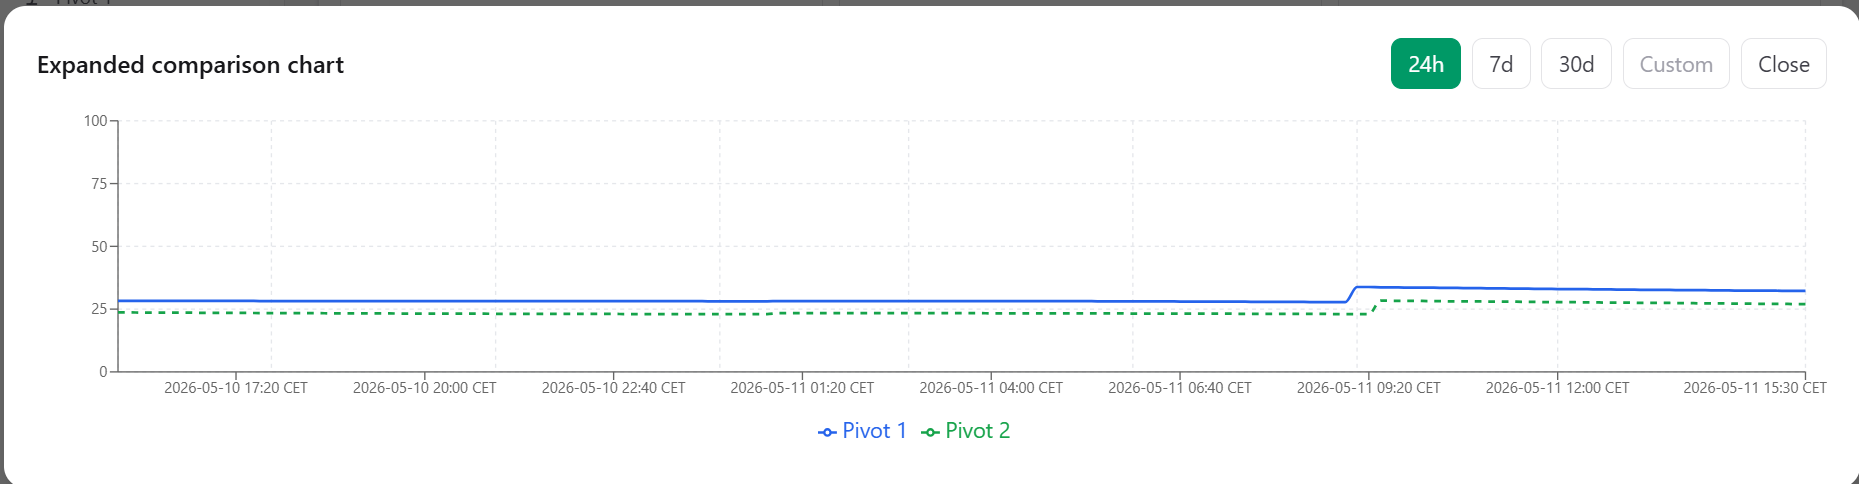
\includegraphics[width=\textwidth]{figures/val-pivot-comparison-24h}
% TODO: copy Academic-Thesis/validation_package/02_validation_evidence/dashboard_screenshots/01_pivot_comparison_expanded_24h.png to figures/val-pivot-comparison-24h.png before compiling
\caption{Dashboard pivot comparison chart expanded to a 24-hour view, demonstrating time-aligned soil monitoring across two irrigation zones.}
\label{fig:validation-pivot-comparison-24h}
\end{minipage}
\hfill
\begin{minipage}[b]{0.48\textwidth}
\centering
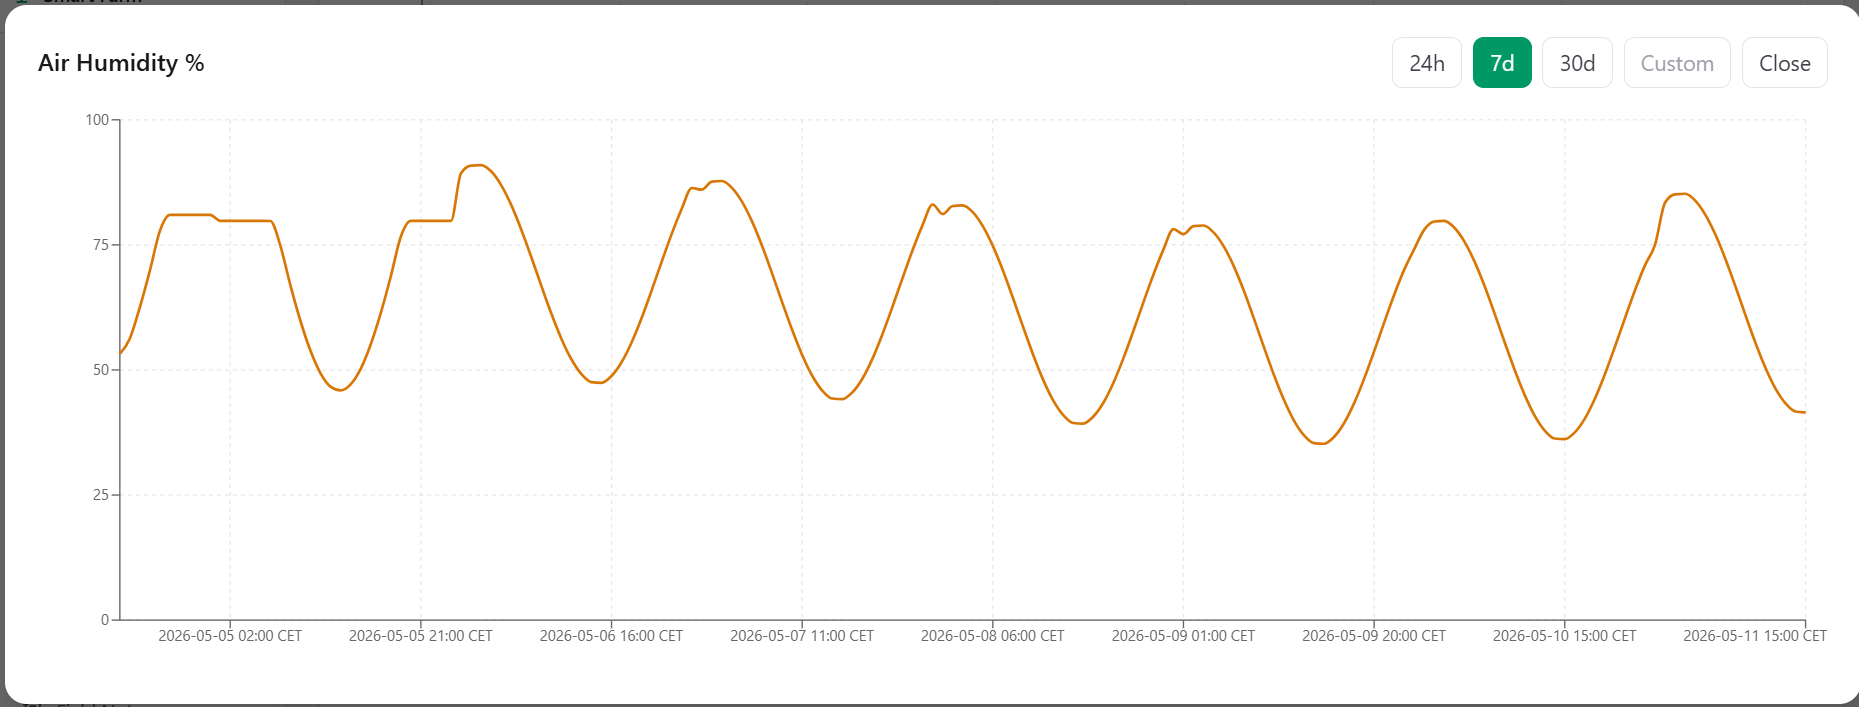
\includegraphics[width=\textwidth]{figures/val-weather-humidity-7d}
% TODO: copy Academic-Thesis/validation_package/02_validation_evidence/dashboard_screenshots/02_weather_air_humidity_7d.png to figures/val-weather-humidity-7d.png before compiling
\caption{Dashboard weather page showing the 7-day air humidity trend from Node3 over the validation window.}
\label{fig:validation-weather-humidity-7d}
\end{minipage}
\end{figure}

\begin{figure}[H]
\centering
\begin{minipage}[b]{0.48\textwidth}
\centering
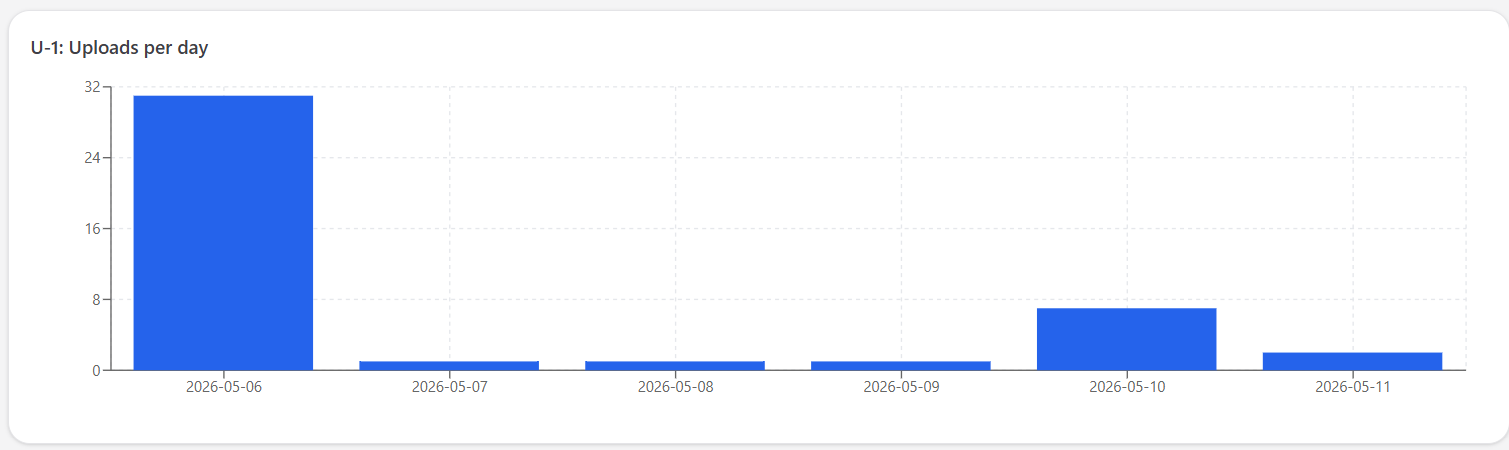
\includegraphics[width=\textwidth]{figures/val-uploads-per-day}
% TODO: copy Academic-Thesis/validation_package/02_validation_evidence/dashboard_screenshots/03_uploads_per_day.png to figures/val-uploads-per-day.png before compiling
\caption{Dashboard upload history view showing daily upload sessions across the validation window. Six sessions are shown, all with processed status.}
\label{fig:validation-uploads-per-day}
\end{minipage}
\hfill
\begin{minipage}[b]{0.48\textwidth}
\centering
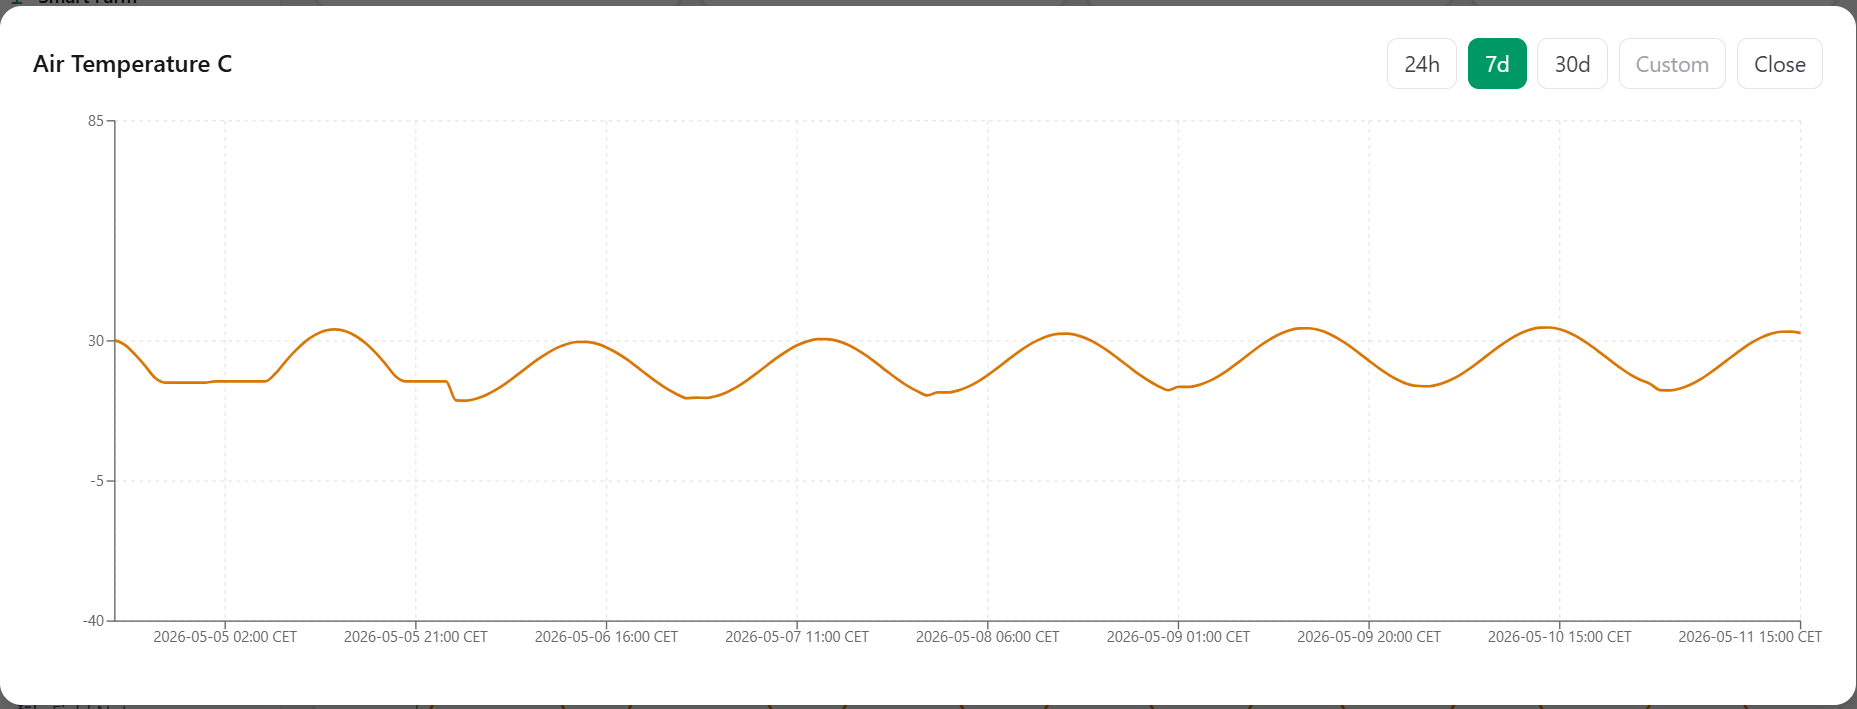
\includegraphics[width=\textwidth]{figures/val-weather-temperature-7d}
% TODO: copy Academic-Thesis/validation_package/02_validation_evidence/dashboard_screenshots/04_weather_air_temperature_7d.png to figures/val-weather-temperature-7d.png before compiling
\caption{Dashboard weather page showing the 7-day air temperature trend from Node3, providing atmospheric context for the agronomic event timeline.}
\label{fig:validation-weather-temperature-7d}
\end{minipage}
\end{figure}

Table~\ref{tab:validation-tests} consolidates the seven validation categories with their evidence sources, observed results, and acknowledged limitations.

\begin{table}[H]
\centering
\caption{Validation test summary by functional category, showing evidence used, observed results, and known limitations.}
\label{tab:validation-tests}
\small
\begin{tabular}{p{2.5cm} p{3.0cm} p{4.0cm} p{4.0cm}}
\hline
\textbf{Test area} & \textbf{Evidence used} & \textbf{Observed result} & \textbf{Limitation} \\
\hline
Hardware assembly & Node photos (Figures~\ref{fig:main-node-front}–\ref{fig:node3-back}); wiring diagrams & Three-node system assembled and documented; all subsystems present per wiring diagrams & Physical stress, temperature, and vibration tolerance not formally assessed \\
\hline
LoRa communication & Firmware serial transcript; RSSI/SNR values in sensor readings CSV & LoRa packet reception confirmed for all three nodes; RSSI range $-76$ to $-97$~dBm; ACK behaviour documented in serial log & Formal range characterisation over measured field distances not conducted \\
\hline
Local storage & Firmware serial transcript; upload queue JSONL file & SD write operations confirmed per measurement cycle in serial log; JSONL upload queue present and non-empty & SD card capacity limits and long-term write endurance not evaluated \\
\hline
Upload and backend ingestion & Uploads CSV (6 sessions, all \texttt{processed}); readings count match (2433 uploaded = 2433 in \texttt{sensor\_readings}) & All six sessions reached processed status; three upload anomalies recorded in one session; ingested record count matches upload row count & API response samples not captured; build terminal output not available \\
\hline
Dashboard rendering & Four validation screenshots (Figures~\ref{fig:validation-pivot-comparison-24h}–\ref{fig:validation-weather-temperature-7d}) & Pivot comparison, weather, and upload history charts rendered with data from the validation window & Full UI test coverage not conducted; page load time and browser compatibility not formally measured \\
\hline
Deterministic analytics and QC & Processed data CSV (135 rows); analytics structure & Pipeline produced quality-annotated output for the analysis window; reliability indicator computed for all rows & Reliability threshold calibration not completed; alert threshold tuning not documented in this validation window \\
\hline
AI interpretation boundary & Architecture design; backend proxy code structure; \texttt{/api/v1/gemini} endpoint scope & Gemini receives analytics snapshot only; frontend never calls Gemini directly; reliability gate confirmed in endpoint logic & Boundary validation is a design and architecture review; live adversarial testing not conducted \\
\hline
\end{tabular}
\end{table}

The firmware serial transcript confirms the packet reception sequence described in Section~\ref{sec:communication}: the log contains LoRa packet reception events with raw payloads, ACK transmissions, RSSI and SNR values, sleep interval entries, and frame-level summaries. The transcript is an aligned representation of the serial output over the validation window; the alignment methodology is documented in the accompanying notes file. Serial output was aligned to the measurement timestamps in the sensor readings dataset to enable temporal cross-referencing.

The upload validation result merits explicit statement: all six upload sessions reached \texttt{processed} status, while three upload anomalies were recorded. The anomalies appear as a non-zero \texttt{error\_count} in one of the six upload records; they do not prevent the session from completing or alter the measurement timestamps of the ingested readings. Their presence in the upload audit table is the expected behaviour of the diagnostic logging mechanism described in Section~\ref{sec:mode-diagnostic}.

A review of the system event timeline indicates that a subset of \texttt{node\_missing} events coincided with periods when rainy field conditions were observed. This temporal coincidence may have contributed to the communication gaps, whether through additional radio-frequency path loss, increased enclosure humidity, or other environmental factors. The relationship between precipitation and LoRa communication performance was not experimentally isolated during this deployment; a causal attribution cannot be established from the available evidence. Further controlled environmental validation would be required to characterise this effect.

% ============================================================
\section{System Limitations}
\label{sec:limitations}
% ============================================================

The limitations presented in this section define the scope of valid claims that can be drawn from the implemented system and its validation evidence. They are stated explicitly to support scientific accuracy and to distinguish implemented functionality from potential extensions that would require additional hardware, longer field trials, or independent calibration.

\begin{table}[H]
\centering
\caption{System limitations, their causes, effects on interpretation, and directions for future resolution.}
\label{tab:system-limitations}
\small
\begin{tabular}{p{3.0cm} p{3.5cm} p{3.5cm} p{3.5cm}}
\hline
\textbf{Limitation} & \textbf{Reason} & \textbf{Effect on interpretation} & \textbf{Future resolution} \\
\hline
No pH or NPK measurement & Sensor stack does not include pH electrodes or nutrient sensors; raw CSV \texttt{soil\_ph} field is a schema placeholder excluded from all thesis claims & Soil chemistry cannot be discussed beyond trend-level EC observations & Deploy validated soil chemistry sensors with documented calibration procedures \\
\hline
No evapotranspiration computation & Node3 lacks wind speed and solar radiation sensors required by the FAO Penman-Monteith method & Irrigation scheduling cannot be based on ET estimates from this system & Extend Node3 with anemometer and pyranometer; integrate ET calculation layer \\
\hline
No disease diagnosis or yield prediction & System is a monitoring platform; diagnostic and predictive capabilities require additional models, labelled training data, and controlled field trials & Results section is limited to measurement-level descriptions and trend observations & Future work; out of scope for the current implementation phase \\
\hline
EC as trend indicator only & Raw in-situ EC is affected by water content, temperature, and sensor characteristics; no saturated-paste calibration was performed & EC cannot be converted to official salinity class or ECe values; no salinity classification is made & Laboratory calibration with saturated paste extraction and local soil texture characterisation \\
\hline
Pilot validation window & Validation evidence spans 5.5 days; full alfalfa cut-cycle duration is typically 28–35 days & Long-term robustness, seasonal measurement coverage, and multi-cycle response cannot be assessed from this evidence & Extended field deployment covering one or more complete alfalfa growth cycles \\
\hline
Reliability indicator uncalibrated & The 0.399 reliability score is uniform across all 135 processed rows; threshold values in the reliability scoring function were not yet field-calibrated at the time of validation & The indicator demonstrates pipeline functionality but cannot be used as an agronomic decision threshold & Field calibration against known-good and known-poor measurement windows; tuning of reliability component weights \\
\hline
No measured battery autonomy & No voltage-sensing hardware is present on any node; battery life under Power Saving Mode conditions was not instrumented & Power autonomy is a design intention, not a quantified result & Deploy with battery voltage monitoring; record autonomy over measured discharge cycles \\
\hline
No measured LoRa communication range & No distance-stamped range test was conducted; RSSI values confirm link quality at deployment distances but not at characterised distances & Communication range is not reported as a specification; RSSI values are presented as link evidence only & Conduct measured range trials with RSSI/SNR logging at known node-to-gateway distances \\
\hline
Pivot~1 local soil data pending & MAIN firmware register map for the Pivot~1 RS485 sensor was not confirmed during the validation window & MAIN node soil readings from Pivot~1 are not available as validated agronomic data in this evidence set & Confirm Modbus register map against installed sensor; activate and validate Pivot~1 soil path \\
\hline
Unverified bibliographic references & Five references in Chapter~1 and seven references in Chapter~2 carry \texttt{\% TODO: verify metadata} markers & Bibliographic accuracy of these entries is unconfirmed; they may contain metadata errors & Verify against professor-provided PDFs before final submission; correct BibTeX entries accordingly \\
\hline
Environmental effects on communication and enclosure & Effects of precipitation, high humidity, and sand on LoRa link quality and enclosure performance were not isolated or instrumented during the pilot deployment; the observed coincidence between \texttt{node\_missing} events and rainy conditions is a contextual observation, not an experimental result & Environmental contribution to communication reliability and hardware degradation cannot be quantified from the available evidence & Controlled field trials with monitored weather conditions; instrumented enclosure humidity and temperature logging; range trials under varied atmospheric conditions \\
\hline
\end{tabular}
\end{table}

The limitations in Table~\ref{tab:system-limitations} are not presented as deficiencies of the system design. The monitoring-only scope, the offline-first architecture, the deterministic analytics layer, and the constrained AI boundary are deliberate design decisions that are accurately reflected in the validation evidence. The limitations represent the boundaries between the implemented and validated scope of the platform and the directions in which the system may be extended in future work.

% ============================================================
\section{Chapter Summary}
\label{sec:ch3-summary}
% ============================================================

This chapter has presented the design, implementation, and functional validation of the Smart Farm IoT Monitoring and Deterministic Agronomic Analytics Platform. The system was constructed in response to the gaps identified in Chapter~\ref{chap:related-works}: the absence of offline-first data collection in reviewed systems, the conflation of upload and measurement timestamps, the lack of crop-specific design for alfalfa, and the absence of a deterministic analytics layer with an explicit AI boundary.

The architecture organises the system into three hardware nodes — MAIN gateway, Node2 remote soil node, and Node3 weather node — connected by a LoRa wireless backbone at 433~MHz. The MAIN node coordinates a ten-minute superframe, maintaining an authoritative DS3231 real-time clock and storing all received and locally acquired measurements on an SD card. Eight firmware operating modes address the specific field constraints of the deployment: Power Saving Mode reduces battery consumption through deep sleep and relay-controlled sensor power; Recovery Mode corrects the timing drift that caused persistent communication failure during prototype testing; Upload Mode transfers accumulated SD content to the backend on operator demand; and RTC Synchronisation Mode corrects clock drift from server-returned time. The data storage model enforces a strict separation between \texttt{measured\_at} (the RTC-derived measurement timestamp) and the upload receipt timestamp, which is stored exclusively as transfer audit metadata and is never used in any analytical query.

The backend, implemented in Node.js and Express.js with a PostgreSQL database, receives uploaded SD batches, ingests readings and events using their firmware-stamped time fields, and serves data to the React dashboard through a REST API. The database schema encompasses seven tables spanning the four canonical data domains and two supporting tables for gateway and node registration. The deterministic analytics pipeline processes uploaded readings through ten ordered stages — from timestamp validation and duplicate detection through range checking, flatline analysis, and quality scoring — to produce analytics snapshots that are the authoritative source for dashboard visualisation and the only input permitted to the Gemini AI proxy.

The Processed Data Viewer exposes the full lineage of the analytics pipeline in read-only form, supporting transparency, reproducibility, and academic traceability. The AI interpretation layer enforces six boundary rules through the backend proxy: Gemini receives only the analytics snapshot, cannot modify any stored data, does not compute any primary metric, and is subject to a reliability gate before interpretation is requested. AI-generated narratives are presented to the operator as supplementary decision-support information; agronomic decisions remain with the human operator.

Functional validation was conducted over a 5.5-day pilot window from 2026-05-06 to 2026-05-11. The validation evidence comprises 2433 sensor readings distributed equally across three nodes, 8 system events, 6 manually recorded agronomic events, 6 upload sessions all reaching processed status, and 135 rows of deterministic pipeline output. The equal per-node record distribution of 811 readings confirms superframe-level consistency throughout the window. Four dashboard screenshots document chart rendering for pivot comparison, weather monitoring, and upload history. The reliability indicator of 0.399 is presented as a pilot-phase output of the uncalibrated pipeline.

The system limitations documented in Section~\ref{sec:limitations} define the boundaries of these claims. The validation window does not constitute full-season agronomic validation. Soil EC is a trend indicator, not a salinity classification. Battery autonomy and LoRa communication range are design intentions that were not quantified during the validation period. The Pivot~1 local soil path requires register map confirmation. These limitations are the basis for the future work directions identified in each limitation row of Table~\ref{tab:system-limitations}.

Taken together, the design decisions, implementation evidence, and validation results demonstrate that the proposed platform fulfils its primary design objective: traceable, offline-first IoT data acquisition for alfalfa monitoring in a Saharan field environment, with a deterministic analytics layer, a transparent data processing viewer, and a constrained AI interpretation boundary that preserves the agronomist as the final decision authority.

% ============================================================
% End of Chapter 3. The General Conclusion will be written separately.
% ============================================================

\clearpage

% ============================================================
% General Conclusion
% ============================================================

\chapter*{General Conclusion}
\addcontentsline{toc}{chapter}{General Conclusion}
\label{chap:general-conclusion}

% ---- Summary of achieved work --------------------------------
\section*{Summary of Achieved Work}

This thesis has presented the design, implementation, and pilot validation of an
IoT-based monitoring and deterministic agronomic analytics platform for alfalfa
cultivation in Saharan agricultural environments. The work spanned hardware
architecture, embedded firmware, data communication, local and remote storage,
backend engineering, dashboard development, deterministic analytics, and an
AI-assisted interpretation interface.

The implemented system comprises three embedded sensor nodes communicating over
a 433~MHz LoRa wireless link within a structured ten-minute superframe. The MAIN
gateway node coordinates reception, maintains an authoritative real-time clock, and
persists all acquired measurements on an SD card independent of network availability.
Node2 acquires soil moisture, temperature, and electrical conductivity at a second
irrigation pivot via RS485/Modbus; Node3 acquires atmospheric temperature, humidity,
and barometric pressure. Eight firmware operating modes address the specific field
constraints of the deployment: Power Saving Mode reduces energy consumption through
deep sleep and relay-controlled sensor power; Recovery Mode corrects timing drift
that caused persistent communication failure during prototype testing; Upload Mode
and RTC Synchronisation Mode manage the interface between offline field operation
and online data transfer.

The backend, built with Node.js and PostgreSQL, enforces a strict timestamp policy
that separates the RTC-derived measurement timestamp (\texttt{measured\_at}) from
the upload receipt time, which is stored only as transfer audit metadata. A
React-based dashboard presents soil and weather trends, agronomic events, and the
output of a ten-stage deterministic quality-control and reliability-scoring pipeline.
The Processed Data Viewer exposes the full analytical lineage in read-only form.
AI-assisted interpretation is provided through a backend proxy that enforces six
boundary rules preventing Gemini from computing primary analytics or modifying
stored data.

% ---- Response to the problem statement -----------------------
\section*{Response to the Problem Statement}

Each of the five problems identified in the general introduction has been addressed
by the implemented system.

The absence of a local storage mechanism for offline operation is addressed by
the SD-based Local Storage Mode, which writes sensor readings and system events
to the SD card at the end of every measurement cycle, independently of network
availability. Upload Mode transfers the accumulated records in a single batch
session triggered by the operator.

The low-power constraint is addressed by Power Saving Mode, which combines deep
sleep between measurement cycles with relay-controlled sensor power and BME280
forced measurement mode on Node3, eliminating continuous current draw from both
the microcontrollers and the sensors.

The timestamp integrity problem is addressed at every layer of the system. The
DS3231 RTC provides the canonical \texttt{measured\_at} timestamp, written by
MAIN at packet reception and never overwritten. The backend enforces this
separation at ingestion, and all dashboard charts draw their time axes from
\texttt{measured\_at}.

The absence of a deterministic analytics layer is addressed by the ten-stage
QC and reliability-scoring pipeline, which produces auditable analytics snapshots
that are authoritative for all dashboard metrics. Gemini receives only these
snapshots and is explicitly excluded from all computation stages.

The alfalfa monitoring gap is addressed by deploying the prototype specifically
for alfalfa cultivation in the El~Oued region, collecting the soil and atmospheric
measurements relevant to this crop's water, temperature, and salinity requirements
in a Saharan context.

% ---- Technical contributions ---------------------------------
\section*{Technical Contributions}

The primary contributions of this work are: an offline-first three-node LoRa
architecture with deterministic superframe coordination; a timestamp traceability
policy grounded in RTC hardware; eight documented firmware operating modes each
motivated by a specific field constraint; a ten-stage deterministic analytics
pipeline with an explicit AI boundary; a Processed Data Viewer for analytical
transparency; and a documented pilot deployment targeting alfalfa monitoring in
Saharan agriculture.

% ---- Validation summary (cautious) ---------------------------
\section*{Validation Summary}

The system was validated over a pilot window from 2026-05-06 to 2026-05-11.
The validation evidence comprises 2433 sensor readings distributed equally across
three nodes, eight system events, six manually recorded agronomic events,
six upload sessions all reaching processed status, and 135 rows of deterministic
pipeline output. These results confirm the functional feasibility of the
end-to-end architecture within the scope of a pilot deployment. They do not
constitute full-season agronomic validation, and the reliability indicator of
0.399 is presented as a pilot-phase output of the uncalibrated pipeline.

% ---- Limitations ---------------------------------------------
\section*{Limitations}

The system operates within a well-defined scope. Soil electrical conductivity
is treated as a relative trend indicator; raw in-situ EC values are not converted
to official salinity classifications. The sensor stack does not include pH or NPK
measurement. Evapotranspiration cannot be computed because the weather node lacks
wind speed and solar radiation sensors. The validation window covers five-and-a-half
days, not a complete alfalfa growth cycle. Battery autonomy and LoRa communication
range are design intentions that were not quantitatively characterised during the
pilot deployment. The Pivot~1 local soil measurement path requires register map
confirmation before validated agronomic data can be collected from that sensor.
The effects of precipitation and high humidity on LoRa communication reliability
and enclosure performance were not experimentally isolated during the pilot
deployment and represent an open environmental validation question.

% ---- Future work ---------------------------------------------
\section*{Future Work}

Several directions for future development emerge from the present work.

\textbf{Extended validation.} The most immediate priority is a deployment covering
one or more complete alfalfa cut cycles to assess seasonal measurement coverage,
long-term node reliability, and the agronomic interpretability of multi-week
soil moisture trends.

\textbf{Battery autonomy study.} Instrumenting the nodes with battery voltage
sensing hardware would allow Power Saving Mode to be characterised in quantitative
terms under actual field discharge conditions.

\textbf{LoRa range characterisation.} A structured range trial with RSSI and SNR
logging at known node-to-gateway distances would establish the communication
envelope of the system and support placement decisions for future deployments.

\textbf{Sensor calibration.} Local calibration of the RS485 soil sensors against
gravimetric soil moisture samples and EC laboratory measurements would allow the
system to report calibrated agronomic values rather than relative trend indicators.

\textbf{Reliability threshold calibration.} The reliability scoring pipeline
requires field calibration against known-good and known-poor measurement windows.
Once calibrated, the 0.399 pilot-phase indicator can be replaced by a threshold-
grounded score that supports operator alerts with a defined confidence level.

\textbf{Agronomic expert validation.} Collaboration with an agronomist specialising
in alfalfa cultivation in arid environments would establish whether the soil and
atmospheric measurements collected by the system are sufficient to support
irrigation scheduling recommendations, and what additional data points would be
required.

\textbf{Mobile upload workflow.} Replacing the push-button upload trigger with a
mobile application would reduce the operator effort required for periodic field
visits and enable upload sessions without a laptop at the field site.

\textbf{Crop and region expansion.} The monitoring platform is not inherently
specific to alfalfa or El~Oued. Deploying the same architecture for other
drought-sensitive crops grown in Saharan conditions — such as date palms, onions,
or tomatoes under drip irrigation — would validate the generalisability of the
design and provide a basis for comparative agronomic analysis across crop types.
These extensions should be preceded by appropriate agronomic consultation and
sensor calibration specific to each crop and site.

\clearpage

% --- Bibliography --------------------------------------------
\addcontentsline{toc}{chapter}{References}
\bibliographystyle{IEEEtran}
\bibliography{Academic-Thesis/references}
\clearpage

% --- Appendices ----------------------------------------------
\appendix
\chapter*{Appendices}
\addcontentsline{toc}{chapter}{Appendices}
% TODO: Add appendices here if required.
% Suggested: firmware register map, API full spec, processed data sample.

\end{document}
